%\chapter{\Objectivetwoname}
\chapter[Kernel Cross-Spectral Functional Connectivity Network]{KCS-FCnet: Kernel Cross-Spectral Functional Connectivity Network for Automatic EEG Representation in MI-BCI}\label{chapter_2}


Here we propose an end-to-end technique for classifying MI using EEG signals, termed Kernel Cross-Spectral Functional Connectivity Network (KCS-FCnet), as depicted in \cref{fig:contribution2}. Our approach overcomes current DL limitations by introducing a cross-spectral Gaussian functional connectivity data-driven estimator to classify MI tasks from raw data. KCS-FCnet utilizes 1D convolutional layers to extract temporal-frequency features from input channels and a cross-spectral distribution estimation that codes relevant temporal and spectral MI patterns. It also includes a functional connectivity feature map, which improves the interpretability of the model by extracting meaningful pairwise channel relationships. Our approach is evaluated on a publicly available dataset and achieves state-of-the-art results for EEG-based MI classification. Furthermore, it demonstrated robustness to different experimental settings and individual differences. Lastly, our results suggest that the KCS-FCnet architecture is a highly effective method for EEG-based MI classification and can potentially be applied in real-world BCI.

\begin{figure}[h!]
    \centering
    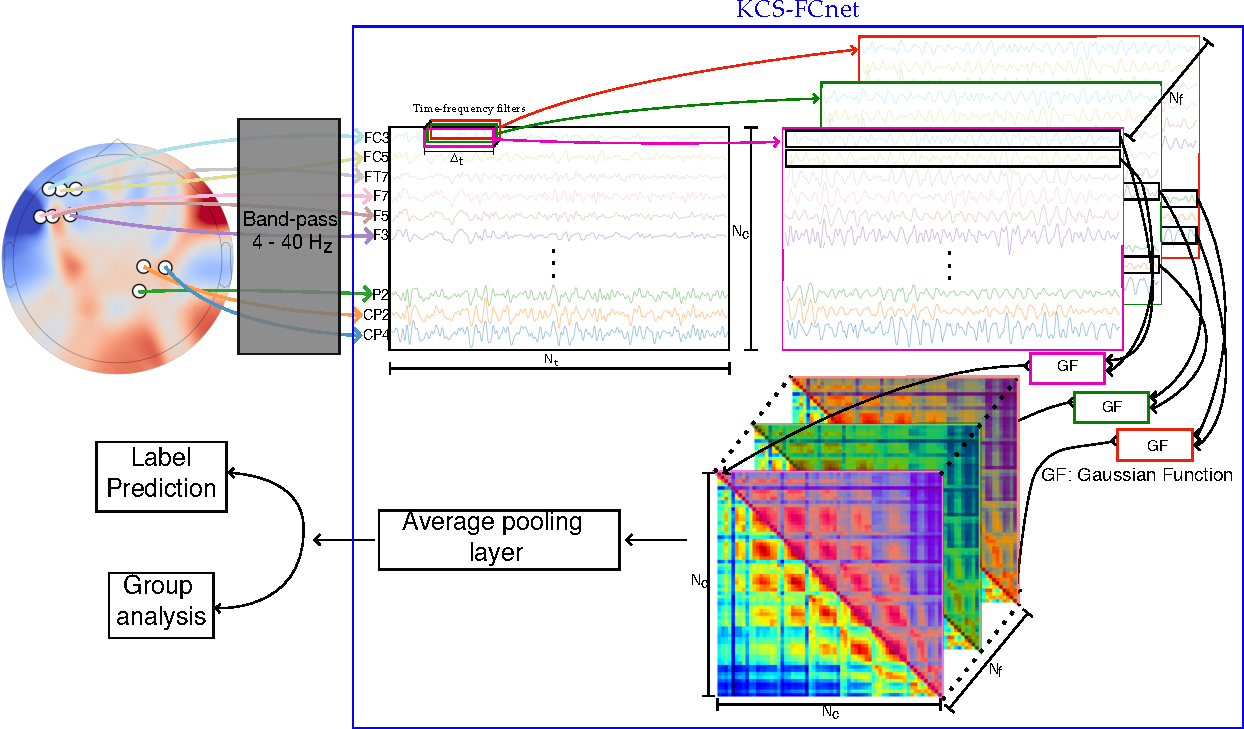
\includegraphics[scale=0.6]{Figures/outline_and_contributions/contribution2.pdf}
    \caption{Schematic diagram illustrating the proposed Kernel Cross-Spectral FC Network (KCS-FCnet), including the use of DL strategies and a CNN layer for artifact removal and spectral and temporal feature extraction. The diagram further outlines the process of spatial extraction via a custom layer incorporating the kernel cross-spectral function}\label{fig:contribution2}
\end{figure}

\section{Kernel Cross-Spectral Functional Connectivity Network}\label{sec:gcnet}
	
	The input-output EEG dataset, $\{\mat{X}_r \in \Real^{N_c \times N_t}, \ve{y}_r \in\{0,1\}^{N_y}\}^R_{r=1}$, comprises $R$ trials, $N_t$ time instants, $N_c$ channels, and $N_y$ classes. To enhance the most informative EEG spatial-temporal-spectral patterns from $\mat{X}_r$ and reduce noise for improved MI class prediction, we propose to estimate the cross-spectral distribution among channels using a function composition. This approach gathers 1-D convolutional-based feature layers for extracting time-frequency patterns within each EEG channel and a Gaussian kernel-based pairwise similarity, as follows:
	\changes{
	\begin{equation}\label{eq:CSf}
		\hat{\mat{P}}_{r}(\ve{w}_f)  = \tilde{K}(\cdot;\sigma) \circ \varphi(\mat{X}_r; \ve{w}_f), 
	\end{equation}
	where $\hat{\mat{P}}_{r}~(\ve{w}_f)~\in~[0,1]^{N_c\times N_c \times N_f}$, $N_f$ is the number of convolutional filters, notation $\circ$ stands for function composition, $\varphi(\cdot; \mat{w}_f)$ is a 1-D convolutional layer that can be used to automatically extract frequency patterns ruled by the weight vector $\ve{w}_f\in \Real^{\Delta_t}$, with $\Delta_t<N_t.$ Of note, in Equation \eqref{eq:CSf} function $\tilde{K}(\cdot;\sigma)$ is the convolutional filter concatenation of all pair-wise values $\kappa_{x}(\ve{x}^{c}_{rf},\ve{x^{c'}_{rf}}; \sigma)$ and is obtained as:
    \begin{equation}
        \tilde{K}(\mat{\tilde{X}}_r;\sigma) = \left[ \mat{K}_{r1} , \mat{K}_{r2}, \cdots,\mat{K}_{rf},\cdots, \mat{K}_{rN_f} \right],
    \end{equation}
    where $\mat{K}_{rf} \in \Real^{N_c \times N_c}$ is the kernel matrix for a trial $r$ at a convolutional filter $f$ and it is calculated as follows:
    \begin{equation}
        \mat{K}_{rf} = \begin{bmatrix}
            \kappa_{x}(\ve{x}^{1}_{rf}, \ve{x}^{1}_{rf}; \sigma) & \kappa_{x}(\ve{x}^{1}_{rf}, \ve{x}^{2}_{rf}; \sigma) & \cdots & \kappa_{x}(\ve{x}^{1}_{rf}, \ve{x}^{N_c}_{rf}; \sigma) \\
            \kappa_{x}(\ve{x}^{2}_{rf}, \ve{x}^{1}_{rf}; \sigma) & \kappa_{x}(\ve{x}^{2}_{rf}, \ve{x}^{2}_{rf}; \sigma) & \cdots & \kappa_{x}(\ve{x}^{2}_{rf}, \ve{x}^{N_c}_{rf}; \sigma) \\
            \vdots & \vdots & \ddots & \vdots \\
            \kappa_{x}(\ve{x}^{N_c}_{rf}, \ve{x}^{1}_{rf}; \sigma) & \kappa_{x}(\ve{x}^{N_c}_{rf}, \ve{x}^{2}_{rf}; \sigma) & \cdots & \kappa_{x}(\ve{x}^{N_c}_{rf}, \ve{x}^{N_c}_{rf}; \sigma).
        \end{bmatrix}
    \end{equation}
    We compute the average functional connectivity measure $\tilde{\mat{P}}_r \in \Real^{N_c \times N_c}$ over convolutional filters, as follows:
    \begin{equation}
		\tilde{\mat{P}}_r  = \operatorname{AvgPooling}_{f} \left(\hat{\mat{P}}_{r}(\ve{w}_f)\right), \label{eq:lastlayerFC}
	\end{equation}
    where $\ve{w}_f$ is the $f$-th convolutional filter, $N_f$ is the number of convolutional filters. This measure provides a way to analyze how different frequency bands of a single-trial EEG relate to each other across channels. After computing the average functional connectivity measure and taking advantage of the symmetric property of the Gaussian functional connectivity, the vectorized version of $\tilde{\mat{P}}_r$ is calculated as:
    \begin{equation} 
        \overline{\ve{p}}_r = \left[\tilde{p}_r^{12}, \tilde{p}_r^{13}, \cdots, \tilde{p}_r^{cc'}, \cdots, \tilde{p}_r^{(N_c-1) N_c} \right]; \forall c<c',
    \end{equation}
    where $\overline{\ve{p}}_r \in  \Real ^{N_c(N_c-1)/2}$. Next, a the softmax-based output layer is applied over vector $\overline{\ve{p}}_r$ to obtain the MI class probability membership $\hat{\ve{y}}_r \in [0,1]^{N_y}$ as:
    }  
    \changes{
	\begin{equation}\label{eq:output}
		\hat{\ve{y}}_r = {\rm{softmax}}\left(\mat{V}\overline{\ve{p}}_r + \ve{b}\right),
	\end{equation}
	where $\mat{V}\in \Real^{N_c(N_c-1)/2\times N_y}$, $\ve{b} \in \Real^{N_y}$. In addition, a gradient descent-based framework using back-propagation is employed to optimize the parameter set $\Theta=\{\ve{w}_f,\mat{V},\ve{b},\sigma;\forall f\in\{1,2,\dots,N_f\}\},$ as follows~\cite{zhang2021dive}:
    }
    
	\begin{equation}\label{eq:opt}
		\Theta^{*} = \underset{\Theta}{\arg\,\min} \quad \promeddd{r}{\mathcal{L}(\ve{y}_r,\hat{\ve{y}}_r|\Theta); \forall r\in\{1,2,\dots,R\}},
	\end{equation}
	being $\mathcal{L} \{\cdot\}$ a given loss function, i.e., cross-entropy. The optimization problem outlined in Equation~\eqref{eq:opt} enables the training of our Kernel Cross-Spectral Functional Connectivity Network (KCS-FCnet) for the classification of MI tasks. 


\section{Experimental Set-Up} \label{sec:Experiment}

\subsection{KCS-FCnet Implementation Details}

In this study, we evaluate the efficacy of our proposed method for extracting subject-specific functional connectivity matrices from the KCS-FCnet that predicts MI output labels from EEG records. To accomplish this, we have developed a pipeline consisting of the following steps, which were tested on the Giga dataset (as detailed in Section \ref{sec:dataset}): 

\begin{itemize}
    \item[--] {{Raw EEG Preprocessing:} 
    } First, we load subject recordings using a \changes{custom database loader} {module} 
    ~(\url{https://github.com/UN-GCPDS/python-gcpds.databases} ({accessed on 27 January 2023}
    )). Next, we downsample each signal from 512 Hz to 128 Hz using the Fourier method provided by the SciPy signal resample function~(\url{https://docs.scipy.org/doc/scipy/reference/generated/scipy.signal.resample.html} ). Then each time series trial was filtered between [4, 40] Hz, using a fifth-order Butterworth bandpass filter. In addition, we clipped the records from 0.5 s to 2.5 s post cue onset, retaining only information from the motor imagery task. Preprocessing step resembles the one provided by authors in~\cite{lawhern2018eegnet}. Note that since we are analyzing only the MI time segment, we assume the signal to be stationary. Our straightforward preprocessing aims to investigate five distinct brain rhythms within the 4 to 40 Hz range, including theta, alpha, and three beta waves. Theta waves (4--8 Hz), located in the hippocampus and various cortical structures, are believed to indicate an ``online state'' and are associated with sensorimotor and mnemonic functions, as stated by authors in \cite{ABHANG201651}. In contrast, sensory stimulation and movements suppress alpha-band activity (8--13 Hz). It is modulated by attention, working memory, and mental tasks, potentially serving as a marker for higher motor control functions. Besides, tested preprocessing also comprises three types of beta waves: Low beta waves (12--15 Hz) or ``beta one'' waves, mainly associated with focused and introverted concentration. Second, mid-range beta waves (15--20 Hz), or ``beta two'' waves, are linked to increased energy, anxiety, and performance. Third, high beta waves (18--40 Hz), or ``beta three'' waves, are associated with significant stress, anxiety, paranoia, high energy, and high arousal.
    
    \item[--] {{KCS-FCnet Training:}} We split trials within each subject data using the standard $5$-{fold} $80${--}$20$ scheme. That means shuffling the data and taking $80\%$ of it to train (training set), holding out the remaining $20\%$ to validate trained models (testing set), and repeating the process five times \cite{schirrmeister2017deep}. For the sake of comparison, we calculate the accuracy, Cohen's kappa, and the area under the ROC curve to compare performance between models~\cite{warrens2015five,geron2022hands}. It is worth noting that we rescale the kernel length according to the new sampling frequency as in \cite{lawhern2018eegnet}. The GridSearchCV class from SKlearn is used to find the best hyperparameter combination of our KCS-FCnet. The number of filters $N_f$ is searched within the set $\{2,3,4\}$.
    
    \item[--] {{Group-Level Analysis:}}  We build a scoring matrix that contains as many rows as subjects in the dataset, 50 for Giga, and six columns, including accuracy, Cohen's kappa, and the area under the ROC curve scores, along with their respective standard deviation. To keep the intuition of the higher, the better, and constrain all columns to be between $[0,1]$ in the score matrix, we replace the standard deviation with its complement and normalize the Cohen's kappa by adding to it the unit and dividing by two. Then, using the score matrix and the k-means clustering algorithm~\cite{geron2022hands}, with $k$ set as three, we trained a model to cluster subjects' results based on the baseline model EEGnet~\cite{lawhern2018eegnet} in one of three groups: best, intermediate, and worst performing subjects. Next, we order each subject based on a projected vector obtained from the first component of the well-known Principal Component Analysis (PCA) algorithm applied to the score matrix. Next, with the trained $k$-means, the subjects analyzed by our KCS-FCnet were clustered using the score matrix. The aim is to compare and check how subjects change between EEGnet and KCS-FCnet-based groups. 
\end{itemize}    
	
A KCS-FCnet sketch can be visualized in \changes{Figure \ref{fig:contribution2}.} The detailed KCS-FCnet architecture is summarized in Table \ref{table:CS-GFCnet}. All experiments were carried out in{ Python 3.8}, with the {Tensorflow 2.4.1 API}, on Google Colaboratory and Kaggle environments. The fine-tuning process for the model's parameters begins by utilizing the training set for optimization. To evaluate the model's performance, the test set is employed solely for reporting scores. The categorical cross-entropy loss function is applied, and no additional callbacks are utilized. The training phase involves passing the entire batch of samples. Additionally, to support further analysis and experimentation, the model weights and performance scores are systematically saved for future reference.

%KCS-FCnet 
	\begin{table}[H]
		\centering
		\caption{Detailed KCS-FCnet architecture for MI classification.}\label{table:CS-GFCnet}
		\begin{tabularx}{\textwidth}{lcc}
			\hline
			\textbf{Layer}     & \textbf{Output Dimension}           & \textbf{Params.}                                                       \\ \midrule
			Input              & $N_c \times N_t \times 1$                 & $\cdot$                                                                  \\
			Conv2D             & $N_c \times (N_t - \Delta_t + 1) \times N_f$     & \begin{tabular}[c]{@{}c@{}}max norm = 2.0, kernel size = (1, $\Delta_t$)\\ Stride size = (1, 1), Bias = False\end{tabular} \\
			BatchNormalization & $N_c \times (N_t - \Delta_t + 1) \times N_f$     & $\cdot$                                                                  \\ \midrule
			\multicolumn{3}{c}{ELU activation}                                                                                               \\ \midrule
			KCS-FCblock           & $N_f \times (N_c \cdot (N_c-1)/2) \times 1$ & $\cdot$                                                                  \\
			AveragePooling2D   & $1 \times (N_c \cdot (N_c-1)/2) \times 1$  & $\cdot$                                                                  \\
			BatchNormalization & $1 \times (N_c \cdot (N_c-1)/2) \times 1$  & $\cdot$                                                                  \\ \midrule
			\multicolumn{3}{c}{ELU activation}                                                                                               \\ \midrule
			Flatten            & $N_c \cdot (N_c-1)/2$                  & $\cdot$                                                                  \\
			Dropout            & $N_c \cdot (N_c-1)/2$                   & Dropout rate = 0.5                                                    \\
			Dense              & $N_y$                                  & max norm = 0.5                                                        \\ \midrule
			\multicolumn{3}{c}{Softmax}                                                                                                      \\ \midrule
		\end{tabularx}
	\end{table}

	\subsection{Functional Connectivity Pruning and Visualization}
	
	To compare functional connectivity between the groups mentioned above, first, we have to check which connections are relevant for class separability. It is worth noting that a high correlation in the functional connectivity matrix does not guarantee a higher class separability. Therefore, we use the two-sample Kolmogorov–Smirnov (2KS) test to overcome this issue and select only relevant connections as in \cite{gu2020random}. The null hypothesis is that both samples are drawn from the same unknown distribution. Thus, we group the trials of each connection for a subject according to the label to build the samples ``right'' and ``left''. Then, every pair is passed through the 2KS test, and connections holding a $p$-value equal to or lower than $0.05$ are kept. Hence, we can state that both samples came from different distributions and the classes are distinguishable. Next, we build a $p$-value matrix containing the information on whether a connection is relevant. To visualize how each $p$-value matrix changes across subjects and groups, we plot each $p$-value matrix on a 2D visualization, where both dimensions are calculated using the well-known $t$-distributed Stochastic Neighbor Embedding ($t$-SNE) algorithm~\cite{van2008visualizing}, from the SKlearn library, over the EEGnet score matrix. It is noteworthy that the perplexity parameter has been specifically set to a value of ten, while all other parameters have been retained at their default settings.
	
	Next, to effectively depict the connections between various regions of the brain, we employ a specialized connectivity visualizer~(\url{https://github.com/UN-GCPDS/python-gcpds.visualizations} ) which utilizes the Circos plot technique to display only the most significant connections, specifically those that fall within the $99$-th percentile. To further enhance the analysis, we have chosen to plot the subject closest to the centroid of each group, thereby allowing for a detailed examination of one individual from each group.
	
	
	\subsection{Method Comparison}
	
	We compare the proposed KCS-FCnet with four end-to-end DL models that have been reported recently for effectively extracting relevantly explainable information from raw EEG. As with our proposal, the contrasted architectures are selected because they benefit from convolutional layers to extract temporal-frequency features for improving MI classification performance. Namely, (i) the EEGnet architecture in~\cite{lawhern2018eegnet} operates depthwise separable convolutions to reduce the number of training parameters, extracting temporal and spatial convolution features from each channel of a previous feature map; (ii) Shallowconvnet in~\cite{schirrmeister2017deep} incorporates two convolution layers (for sequential bandpass and spatial filtering of the EEG channels) followed by a square and log activation function, an average pooling layer, and a fully connected layer to emulate the baseline strategy of Filter Bank Common Spatial Patterns~\cite{ang2008filter}; (iii) Deepconvnet proposed by~\cite{schirrmeister2017deep} employs three convolutional layers to extract DL features; and (iv) TCNet-Fusion comprises three filtering stages to extract temporal, bandpass spectral, and spatial features, as explained in detail in~\cite{musallam2021electroencephalography}.
	
	For concrete testing, individual subject accuracy and standard deviation scores are only compared between the EEGnet and our KCS-FCnet due to their similarity in architecture and the number of parameters. For all provided approaches, the average classification performance along the 50 subjects in Giga is computed. Every architecture is implemented using TensorFlow2 and the SciKeras library, which allows wrapping any deep learning model as a SKlearn classifier. For the EEGnet, Shallowconvnet, Deepconvnet, and TCNet-Fusion, we use the hyperparameters that each work reported as the best combination. The complete codes for training, validating, and saving the model are publicly available (EEGnet~\footnote{\url{https://www.kaggle.com/dggarciam94/eegnet-11-11-2022-version}}, Shallowconvnet~\footnote{\url{https://www.kaggle.com/dggarciam94/shallownet-11-11-2022-version}}, Deepconvnet~\footnote{\url{https://www.kaggle.com/dggarciam94/deepconvnet-11-11-2022-version}}, TCNet-Fusion~\footnote{\url{https://www.kaggle.com/dggarciam94/tcnet-fusion-11-11-2022-version}}, and KCS-FCnet~\footnote{\url{https://www.kaggle.com/code/dggarciam94/gfcnet-11-11-2022-version)}}.

 \section{Results and Discussion}


\subsection{Subject Dependent and Group Analysis Results}

The proposed KCS-FCnet architecture is closely compared to the EEGnet architecture in this study, with a focus on subject-specific accuracy scores and their standard deviation. The comparison is illustrated in Figure \ref{fig:compeeggfc}, where the dotted orange line represents the EEGnet and the dotted blue line represents the proposed KCS-FCnet. The blue and red bars indicate whether a specific subject's accuracy improves or decreases when using the KCS-FCnet, respectively. Additionally, the background of the figure includes low-opacity green, yellow, and red bars to indicate the group belongingness of the subjects (best, intermediate, and worst-performing clusters). The X-axis of the figure displays the subjects sorted based on their maximum score values as determined by the EEGnet results. The average accuracy for EEGnet and KCS-FCnet is $69.0$ and $76.4$, respectively, resulting in an incremental of $7.4$ for our proposal. Overall, it is demonstrated that KCS-FCnet can effectively classify motor imagery tasks using raw EEG as input data.

\begin{figure}[h!]
    \centering
    \resizebox{\linewidth}{!}{% This file was created with tikzplotlib v0.10.1.
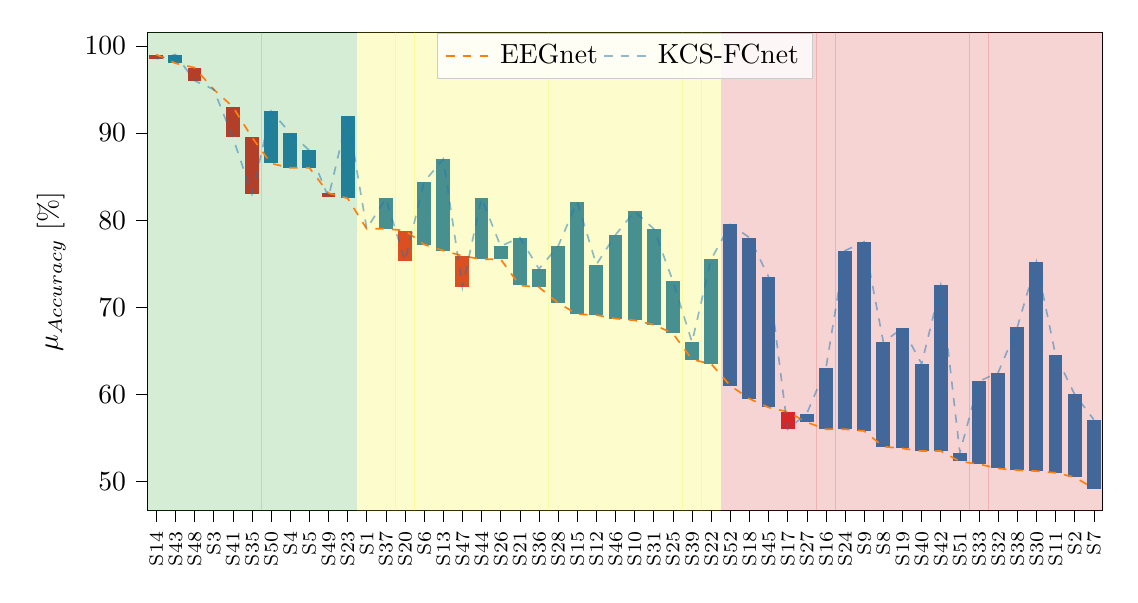
\begin{tikzpicture}

\definecolor{crimson2143940}{RGB}{214,39,40}
\definecolor{darkgray176}{RGB}{176,176,176}
\definecolor{darkorange25512714}{RGB}{255,127,14}
\definecolor{lightgray204}{RGB}{204,204,204}
\definecolor{steelblue31119180}{RGB}{31,119,180}

\definecolor{green}{RGB}{44,160,44}
\definecolor{yellow}{RGB}{240,240,0}
\definecolor{red}{RGB}{214,39,40}

\begin{axis}[
legend cell align={left},
legend cell align={left},
legend columns=2,
legend columns=2,
legend style={
  fill opacity=0.8,
  draw opacity=1,
  text opacity=1,
  at={(0.5,1)},
  anchor=north,
  draw=lightgray204
},
legend style={
  fill opacity=0.8,
  draw opacity=1,
  text opacity=1,
  at={(0.5,1)},
  anchor=north,
  draw=lightgray204
},
tick align=outside,
tick pos=left,
x grid style={darkgray176},
xmin=-0.45, xmax=49.45,
xtick style={color=black},
xtick={0,1,2,3,4,5,6,7,8,9,10,11,12,13,14,15,16,17,18,19,20,21,22,23,24,25,26,27,28,29,30,31,32,33,34,35,36,37,38,39,40,41,42,43,44,45,46,47,48,49},
xticklabel style={rotate=90.0},
xticklabels={\scriptsize
  S14,
  \scriptsize S43,
  \scriptsize S48,
  \scriptsize S3,
  \scriptsize S41,
  \scriptsize S35,
  \scriptsize S50,
  \scriptsize S4,
  \scriptsize S5,
  \scriptsize S49,
  \scriptsize S23,
  \scriptsize S1,
  \scriptsize S37,
  \scriptsize S20,
  \scriptsize S6,
  \scriptsize S13,
  \scriptsize S47,
  \scriptsize S44,
  \scriptsize S26,
  \scriptsize S21,
  \scriptsize S36,
  \scriptsize S28,
  \scriptsize S15,
  \scriptsize S12,
  \scriptsize S46,
  \scriptsize S10,
  \scriptsize S31,
  \scriptsize S25,
  \scriptsize S39,
  \scriptsize S22,
  \scriptsize S52,
  \scriptsize S18,
  \scriptsize S45,
  \scriptsize S17,
  \scriptsize S27,
  \scriptsize S16,
  \scriptsize S24,
  \scriptsize S9,
  \scriptsize S8,
  \scriptsize S19,
  \scriptsize S40,
  \scriptsize S42,
  \scriptsize S51,
  \scriptsize S33,
  \scriptsize S32,
  \scriptsize S38,
  \scriptsize S30,
  \scriptsize S11,
  \scriptsize S2,
  \scriptsize S7
},
y grid style={darkgray176},
ylabel={\(\displaystyle \mu_{Accuracy}\) [\%]},
ymin=46.71, ymax=101.49,
ytick style={color=black},
% only scale the axis, not the axis including the ticks and labels
scale only axis=true,
% set `width' and `height' to the desired values
width=\textwidth,
height=0.5\textwidth,
]

\path [draw=steelblue31119180, line width=5pt]
(axis cs:1,98)
--(axis cs:1,99);

\path [draw=steelblue31119180, line width=5pt]
(axis cs:3,95)
--(axis cs:3,95);



\path [draw=steelblue31119180, line width=5pt]
(axis cs:6,86.5)
--(axis cs:6,92.5);

\path [draw=steelblue31119180, line width=5pt]
(axis cs:7,86)
--(axis cs:7,90);

\path [draw=steelblue31119180, line width=5pt]
(axis cs:8,86)
--(axis cs:8,88);

\path [draw=steelblue31119180, line width=5pt]
(axis cs:10,82.5)
--(axis cs:10,92);

\path [draw=steelblue31119180, line width=5pt]
(axis cs:11,79)
--(axis cs:11,79);

\path [draw=steelblue31119180, line width=5pt]
(axis cs:12,79)
--(axis cs:12,82.5);

\path [draw=steelblue31119180, line width=5pt]
(axis cs:14,77.2)
--(axis cs:14,84.4);

\path [draw=steelblue31119180, line width=5pt]
(axis cs:15,76.5)
--(axis cs:15,87);

\path [draw=steelblue31119180, line width=5pt]
(axis cs:17,75.5)
--(axis cs:17,82.5);

\path [draw=steelblue31119180, line width=5pt]
(axis cs:18,75.5)
--(axis cs:18,77);

\path [draw=steelblue31119180, line width=5pt]
(axis cs:19,72.5)
--(axis cs:19,78);

\path [draw=steelblue31119180, line width=5pt]
(axis cs:20,72.3)
--(axis cs:20,74.4);

\path [draw=steelblue31119180, line width=5pt]
(axis cs:21,70.5)
--(axis cs:21,77);

\path [draw=steelblue31119180, line width=5pt]
(axis cs:22,69.2)
--(axis cs:22,82.1);

\path [draw=steelblue31119180, line width=5pt]
(axis cs:23,69.1)
--(axis cs:23,74.9);

\path [draw=steelblue31119180, line width=5pt]
(axis cs:24,68.7)
--(axis cs:24,78.3);

\path [draw=steelblue31119180, line width=5pt]
(axis cs:25,68.5)
--(axis cs:25,81);

\path [draw=steelblue31119180, line width=5pt]
(axis cs:26,68)
--(axis cs:26,79);

\path [draw=steelblue31119180, line width=5pt]
(axis cs:27,67)
--(axis cs:27,73);

\path [draw=steelblue31119180, line width=5pt]
(axis cs:28,64)
--(axis cs:28,66);

\path [draw=steelblue31119180, line width=5pt]
(axis cs:29,63.5)
--(axis cs:29,75.5);

\path [draw=steelblue31119180, line width=5pt]
(axis cs:30,61)
--(axis cs:30,79.5);

\path [draw=steelblue31119180, line width=5pt]
(axis cs:31,59.5)
--(axis cs:31,78);

\path [draw=steelblue31119180, line width=5pt]
(axis cs:32,58.5)
--(axis cs:32,73.5);

\path [draw=steelblue31119180, line width=5pt]
(axis cs:34,56.8)
--(axis cs:34,57.8);

\path [draw=steelblue31119180, line width=5pt]
(axis cs:35,56)
--(axis cs:35,63);

\path [draw=steelblue31119180, line width=5pt]
(axis cs:36,56)
--(axis cs:36,76.5);

\path [draw=steelblue31119180, line width=5pt]
(axis cs:37,55.8)
--(axis cs:37,77.5);

\path [draw=steelblue31119180, line width=5pt]
(axis cs:38,54)
--(axis cs:38,66);

\path [draw=steelblue31119180, line width=5pt]
(axis cs:39,53.8)
--(axis cs:39,67.6);

\path [draw=steelblue31119180, line width=5pt]
(axis cs:40,53.5)
--(axis cs:40,63.5);

\path [draw=steelblue31119180, line width=5pt]
(axis cs:41,53.5)
--(axis cs:41,72.5);

\path [draw=steelblue31119180, line width=5pt]
(axis cs:42,52.3)
--(axis cs:42,53.3);

\path [draw=steelblue31119180, line width=5pt]
(axis cs:43,52)
--(axis cs:43,61.5);

\path [draw=steelblue31119180, line width=5pt]
(axis cs:44,51.5)
--(axis cs:44,62.5);

\path [draw=steelblue31119180, line width=5pt]
(axis cs:45,51.3)
--(axis cs:45,67.7);

\path [draw=steelblue31119180, line width=5pt]
(axis cs:46,51.2)
--(axis cs:46,75.2);

\path [draw=steelblue31119180, line width=5pt]
(axis cs:47,51)
--(axis cs:47,64.5);

\path [draw=steelblue31119180, line width=5pt]
(axis cs:48,50.5)
--(axis cs:48,60);

\path [draw=steelblue31119180, line width=5pt]
(axis cs:49,49.2)
--(axis cs:49,57.1);

\path [draw=crimson2143940, line width=5pt]
(axis cs:0,99)
--(axis cs:0,98.5);

\path [draw=crimson2143940, line width=5pt]
(axis cs:2,97.5)
--(axis cs:2,96);

\path [draw=crimson2143940, line width=5pt]
(axis cs:4,93)
--(axis cs:4,89.5);

\path [draw=crimson2143940, line width=5pt]
(axis cs:5,89.5)
--(axis cs:5,83);

\path [draw=crimson2143940, line width=5pt]
(axis cs:9,83.1)
--(axis cs:9,82.6);

\path [draw=crimson2143940, line width=5pt]
(axis cs:13,78.8)
--(axis cs:13,75.3);

\path [draw=crimson2143940, line width=5pt]
(axis cs:16,75.9)
--(axis cs:16,72.3);

\path [draw=crimson2143940, line width=5pt]
(axis cs:33,58)
--(axis cs:33,56);

\path [draw=green, opacity=0.2, line width=7pt]
(axis cs:1,45)
--(axis cs:1,105);

\path [draw=green, opacity=0.2, line width=7pt]
(axis cs:0,45)
--(axis cs:0,105);

\path [draw=green, opacity=0.2, line width=7pt]
(axis cs:2,45)
--(axis cs:2,105);

\path [draw=green, opacity=0.2, line width=7pt]
(axis cs:3,45)
--(axis cs:3,105);

\path [draw=green, opacity=0.2, line width=7pt]
(axis cs:4,45)
--(axis cs:4,105);

\path [draw=green, opacity=0.2, line width=7pt]
(axis cs:5,45)
--(axis cs:5,105);

\path [draw=green, opacity=0.2, line width=7pt]
(axis cs:6,45)
--(axis cs:6,105);

\path [draw=green, opacity=0.2, line width=7pt]
(axis cs:7,45)
--(axis cs:7,105);

\path [draw=green, opacity=0.2, line width=7pt]
(axis cs:8,45)
--(axis cs:8,105);

\path [draw=green, opacity=0.2, line width=7pt]
(axis cs:9,45)
--(axis cs:9,105);

\path [draw=green, opacity=0.2, line width=7pt]
(axis cs:10,45)
--(axis cs:10,105);

\path [draw=yellow, opacity=0.2, line width=7pt]
(axis cs:11,45)
--(axis cs:11,105);

\path [draw=yellow, opacity=0.2, line width=7pt]
(axis cs:12,45)
--(axis cs:12,105);

\path [draw=yellow, opacity=0.2, line width=7pt]
(axis cs:13,45)
--(axis cs:13,105);

\path [draw=yellow, opacity=0.2, line width=7pt]
(axis cs:14,45)
--(axis cs:14,105);

\path [draw=yellow, opacity=0.2, line width=7pt]
(axis cs:15,45)
--(axis cs:15,105);

\path [draw=yellow, opacity=0.2, line width=7pt]
(axis cs:16,45)
--(axis cs:16,105);

\path [draw=yellow, opacity=0.2, line width=7pt]
(axis cs:17,45)
--(axis cs:17,105);

\path [draw=yellow, opacity=0.2, line width=7pt]
(axis cs:18,45)
--(axis cs:18,105);

\path [draw=yellow, opacity=0.2, line width=7pt]
(axis cs:19,45)
--(axis cs:19,105);

\path [draw=yellow, opacity=0.2, line width=7pt]
(axis cs:20,45)
--(axis cs:20,105);

\path [draw=yellow, opacity=0.2, line width=7pt]
(axis cs:21,45)
--(axis cs:21,105);

\path [draw=yellow, opacity=0.2, line width=7pt]
(axis cs:22,45)
--(axis cs:22,105);

\path [draw=yellow, opacity=0.2, line width=7pt]
(axis cs:23,45)
--(axis cs:23,105);

\path [draw=yellow, opacity=0.2, line width=7pt]
(axis cs:24,45)
--(axis cs:24,105);

\path [draw=yellow, opacity=0.2, line width=7pt]
(axis cs:25,45)
--(axis cs:25,105);

\path [draw=yellow, opacity=0.2, line width=7pt]
(axis cs:26,45)
--(axis cs:26,105);

\path [draw=yellow, opacity=0.2, line width=7pt]
(axis cs:27,45)
--(axis cs:27,105);

\path [draw=yellow, opacity=0.2, line width=7pt]
(axis cs:28,45)
--(axis cs:28,105);

\path [draw=yellow, opacity=0.2, line width=7pt]
(axis cs:29,45)
--(axis cs:29,105);

\path [draw=red, opacity=0.2, line width=7pt]
(axis cs:30,45)
--(axis cs:30,105);

\path [draw=red, opacity=0.2, line width=7pt]
(axis cs:31,45)
--(axis cs:31,105);

\path [draw=red, opacity=0.2, line width=7pt]
(axis cs:32,45)
--(axis cs:32,105);

\path [draw=red, opacity=0.2, line width=7pt]
(axis cs:33,45)
--(axis cs:33,105);

\path [draw=red, opacity=0.2, line width=7pt]
(axis cs:34,45)
--(axis cs:34,105);

\path [draw=red, opacity=0.2, line width=7pt]
(axis cs:35,45)
--(axis cs:35,105);

\path [draw=red, opacity=0.2, line width=7pt]
(axis cs:36,45)
--(axis cs:36,105);

\path [draw=red, opacity=0.2, line width=7pt]
(axis cs:37,45)
--(axis cs:37,105);

\path [draw=red, opacity=0.2, line width=7pt]
(axis cs:38,45)
--(axis cs:38,105);

\path [draw=red, opacity=0.2, line width=7pt]
(axis cs:39,45)
--(axis cs:39,105);

\path [draw=red, opacity=0.2, line width=7pt]
(axis cs:40,45)
--(axis cs:40,105);

\path [draw=red, opacity=0.2, line width=7pt]
(axis cs:41,45)
--(axis cs:41,105);

\path [draw=red, opacity=0.2, line width=7pt]
(axis cs:42,45)
--(axis cs:42,105);

\path [draw=red, opacity=0.2, line width=7pt]
(axis cs:43,45)
--(axis cs:43,105);

\path [draw=red, opacity=0.2, line width=7pt]
(axis cs:44,45)
--(axis cs:44,105);

\path [draw=red, opacity=0.2, line width=7pt]
(axis cs:45,45)
--(axis cs:45,105);

\path [draw=red, opacity=0.2, line width=7pt]
(axis cs:46,45)
--(axis cs:46,105);

\path [draw=red, opacity=0.2, line width=7pt]
(axis cs:47,45)
--(axis cs:47,105);

\path [draw=red, opacity=0.2, line width=7pt]
(axis cs:48,45)
--(axis cs:48,105);

\path [draw=red, opacity=0.2, line width=7pt]
(axis cs:49,45)
--(axis cs:49,105);

\addplot [semithick, darkorange25512714, dashed]
table {%
0 99
1 98
2 97.5
3 95
4 93
5 89.5
6 86.5
7 86
8 86
9 83.1
10 82.5
11 79
12 79
13 78.8
14 77.2
15 76.5
16 75.9
17 75.5
18 75.5
19 72.5
20 72.3
21 70.5
22 69.2
23 69.1
24 68.7
25 68.5
26 68
27 67
28 64
29 63.5
30 61
31 59.5
32 58.5
33 58
34 56.8
35 56
36 56
37 55.8
38 54
39 53.8
40 53.5
41 53.5
42 52.3
43 52
44 51.5
45 51.3
46 51.2
47 51
48 50.5
49 49.2
};
\addlegendentry{EEGnet}
\addplot [semithick, steelblue31119180, opacity=0.5, dashed]
table {%
0 98.5
1 99
2 96
3 95
4 89.5
5 83
6 92.5
7 90
8 88
9 82.6
10 92
11 79
12 82.5
13 75.3
14 84.4
15 87
16 72.3
17 82.5
18 77
19 78
20 74.4
21 77
22 82.1
23 74.9
24 78.3
25 81
26 79
27 73
28 66
29 75.5
30 79.5
31 78
32 73.5
33 56
34 57.8
35 63
36 76.5
37 77.5
38 66
39 67.6
40 63.5
41 72.5
42 53.3
43 61.5
44 62.5
45 67.7
46 75.2
47 64.5
48 60
49 57.1
};
\addlegendentry{KCS-FCnet}


\end{axis}

\end{tikzpicture}
}
    \caption{Subject specific results. EEGnet and KCS-FCnet average accuracies are depicted, with subjects being sorted based on their performance using   EEGnet. The blue bars represent an improvement in performance using the KCS-FCnet, while the red bars indicate a decrease in performance. The background codes the group membership (best---G I, medium---GII, and worst---GIII performance clusters).}\label{fig:compeeggfc}
\end{figure}


Moreover, our proposed method, KCS-FCnet, demonstrates mixed results in terms of accuracy for the subjects studied. On the one hand, seven subjects experienced a decrease in accuracy, of which only four experienced a reduction of three points or more. On the other hand, the remaining subjects experience an increase in accuracy, with the majority experiencing an increase of more than five points. Notably, our approach has a particularly strong impact on subjects in the third group, resulting in only one case where KCS-FCnet fails to surpass the baseline performance and two cases with less than one point of increase. Additionally, our data-driven functional connectivity method proves effective in extracting relevant feature maps for subjects in the second group, with over ten subjects experiencing an accuracy increment of at least three points. The first group, consisting of subjects with good performance, does not see remarkable results from KCS-FCnet, with only one subject experiencing a decrease in performance by five points and one subject experiencing an increase of more than five points. In general, subjects with the best performance appear to have a limitation when trying to include more relevant feature maps, yet our network is able to preserve their classification performance in most cases. In contrast, poor-performance subjects have more room for enhancement in the feature map, which is why we see a more significant increment in the third group.
	
Figure \ref{fig:belongcomp} illustrates the subject group belongingness and the impact of the KCS-FCnet method on group classification. The first row shows the subjects organized based on the EEGnet results, while the bottom row shows how each subject changes or maintains their group based on the KCS-FCnet results. For example, in the red group on the EEGnet row, subjects starting from S52, when we look at the new grouping based on KCS-FCnet for the same subset of subjects, it is evident that a total of eleven subjects significantly improved their performance, moving to the yellow cluster, while only nine remained in the red one. Additionally, six subjects had a major performance increase and were promoted to the best group (green), which demonstrates the effectiveness of the proposed framework. Furthermore, the subjects that were originally in the best group maintained their status, indicating that the best-performing subjects are less likely to improve. Then, our approach achieves better MI discrimination compared to EEGnet, particularly for bad and medium-performing subjects, which is important as it highlights the model's capacity to handle challenging cases. 

%semaforo cambio grupos
\begin{figure}[h!]
    \centering
    \resizebox{\linewidth}{!}{% This file was created with tikzplotlib v0.10.1.
\begin{tikzpicture}

\definecolor{darkgray176}{RGB}{176,176,176}

\begin{axis}[
tick align=outside,
tick pos=left,
width=1\textwidth,
height=.5\textwidth,
x grid style={darkgray176},
xmin=-0.5, xmax=49.5,
xtick style={color=black},
xtick={0,1,2,3,4,5,6,7,8,9,10,11,12,13,14,15,16,17,18,19,20,21,22,23,24,25,26,27,28,29,30,31,32,33,34,35,36,37,38,39,40,41,42,43,44,45,46,47,48,49},
xticklabel style={rotate=90.0},
xticklabels={
  S20,
  S40,
  S38,
  S48,
  S8,
  S45,
  S11,
  S3,
  S41,
  S30,
  S15,
  S14,
  S27,
  S21,
  S35,
  S37,
  S32,
  S10,
  S42,
  S36,
  S17,
  S25,
  S6,
  S1,
  S33,
  S49,
  S22,
  S46,
  S24,
  S28,
  S7,
  S26,
  S51,
  S47,
  S31,
  S13,
  S12,
  S5,
  S4,
  S44,
  S9,
  S19,
  S2,
  S18,
  S52,
  S16,
  S39,
  S23,
  S43,
  S50
},
y dir=reverse,
y grid style={darkgray176},
ymin=-0.5, ymax=2.5,
ytick style={color=black},
ytick={0,1,2},
yticklabels={EEGnet,KCS-FCnet,RKCS-FCnet}
]
\addplot graphics [includegraphics cmd=\pgfimage,xmin=-0.5, xmax=49.5, ymin=2.5, ymax=-0.5] {Figures/Objective_3/semaforo.png};
\end{axis}

\end{tikzpicture}
}
    \caption{KCS-FCnet subject group enhancement regarding the EEGnet performance. Note that green, yellow and red represent best, medium, and worst performance regarding the average accuracy along subjects. First row: Subjects organized based on the EEGnet classification. Second row: Subject membership changes based on the KCS-FCnet results. }\label{fig:belongcomp}
\end{figure}


Next, Table \ref{tab:groupacc} shows the accuracy results for each group for EEGnet and KCS-FCnet. It is important to note that while the difference in the first group is insignificant, with only $0.9$ points, there is a notable improvement in the second group, with an increment of 5.6 accuracy points. Additionally, the third group shows a considerable increment of $12.4$ points. A similar trend is observed in the standard deviation, where the second group has the most reduction of $2.6$ points. Hence, our proposal not only outperforms EEGnet in terms of accuracy but also reduces the variability for all clusters.
	
	

\begin{table}[h!] 
    \caption{{Group}%MDPI: Please check if the background color is unnecessary for tables and can be removed. Ans removed 
        -based accuracy results for EEGnet and KCS-FCnet. The average accuracy for the best, medium, and worst-grouped subjects is depicted. The KCS-FCnet average increase for each cluster is also reported.\label{tab:groupacc}}
    \newcolumntype{W}{>{\centering\arraybackslash}X}
    \begin{tabularx}{\textwidth}{WWWW}
        \toprule
        \textbf{Approach}                    & \textbf{Group}                         & \textbf{Accuracy}                              &  \textbf{KCS-FCnet Gain}                 \\ \hline
        \multirow{3}{*}{EEGnet}                        & G I   & $90.6 \pm 4.3$                                  & $\cdot$                             \\ \cline{2-4} 
        & G II  & $72.2  \pm 7.3$                                & $\cdot$                                 \\ \cline{2-4} 
        & G III & $54.3 \pm 6.6$                                 & $\cdot$                                  \\ \hline
        
        
        
        
        \multirow{3}{*}{KCS-FCnet}                      & G I   & \textbf{$91.5 \pm 3.3$} & \textbf{{0.9} %MDPI: Please add an explanation for bold in the table footer. If the bold is unnecessary, please remove it. 
        } \\ \cline{2-4} 
        & G II  & \textbf{$77.8 \pm 4.7$} & \textbf{{5.6}} \\ \cline{2-4} 
        & G III & \textbf{$66.7 \pm 5.6$} & \textbf{{12.4}} \\
        
        
        
        
        
        \noalign{\hrule height 0.5pt}
    \end{tabularx}
\end{table}




Figure \ref{fig:stdcompeeggfc} compares the accuracy standard deviation for EEGnet and KCS-FCnet. The background boxes indicate the group membership. For the first group, we can see an improvement in the variability scores for our proposed method, with a difference of four points between the maximum values. The second group shows a slight reduction in all standard deviation values for our method; however, the variability proportion remains almost the same. For the last group, there is a similar behavior for both methods. Overall, our proposed strategy reduces the variability and maintains a similar average accuracy score among subjects in the best group while increasing the average accuracy and maintaining the variability for the second and third clusters.

%variability results
\begin{figure}[h!]
    \centering
    \resizebox{0.8\linewidth}{!}{% This file was created with tikzplotlib v0.10.1.
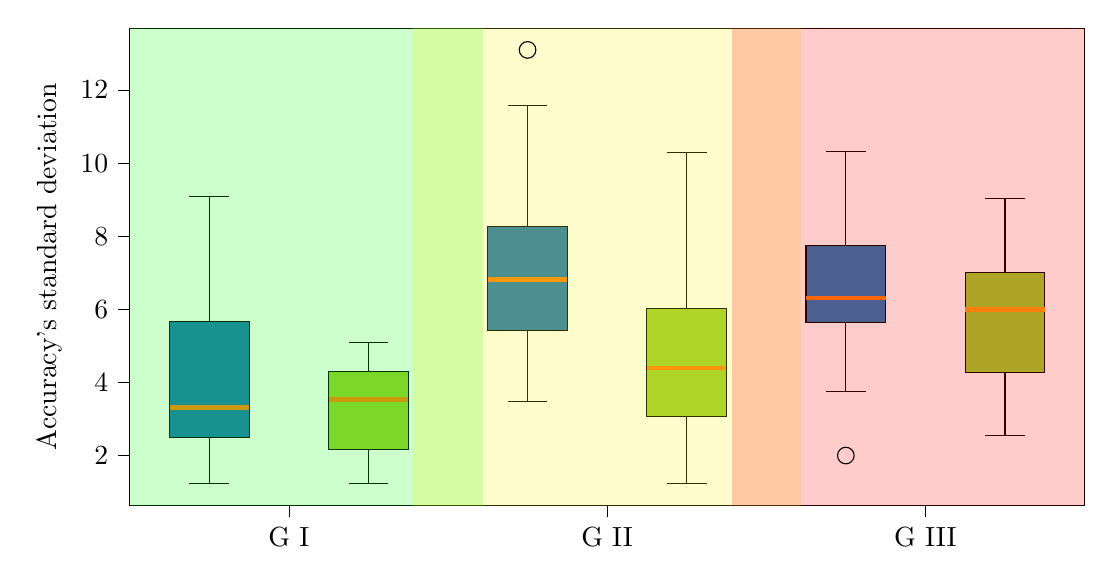
\begin{tikzpicture}

\definecolor{darkgray176}{RGB}{176,176,176}
\definecolor{darkorange25512714}{RGB}{255,127,14}
\definecolor{steelblue31119180}{RGB}{31,119,180}
\definecolor{yellowgreen}{RGB}{154, 205, 50}


\begin{axis}[
tick align=outside,
tick pos=left,
x grid style={darkgray176},
xmin=0.5, xmax=6.5,
xtick style={color=black},
y grid style={darkgray176},
ymin=0.63119207227573, ymax=13.6893536528247,
ytick style={color=black},
xtick={1.5,3.5,5.5},
xticklabels={
  G I,
  G II,
  G III
  },
  ylabel=Accuracy's standard deviation,
% only scale the axis, not the axis including the ticks and labels
scale only axis=true,
% set `width' and `height' to the desired values
width=\textwidth,
height=0.5\textwidth,
]
\path [draw=black, fill=steelblue31119180]
(axis cs:0.75,2.49949974978979)
--(axis cs:1.25,2.49949974978979)
--(axis cs:1.25,5.66066665775428)
--(axis cs:0.75,5.66066665775428)
--(axis cs:0.75,2.49949974978979)
--cycle;
\addplot [black]
table {%
1 2.49949974978979
1 1.22474487139159
};
\addplot [black]
table {%
1 5.66066665775428
1 9.08295106229247
};
\addplot [black]
table {%
0.875 1.22474487139159
1.125 1.22474487139159
};
\addplot [black]
table {%
0.875 9.08295106229247
1.125 9.08295106229247
};
\path [draw=black, fill=yellowgreen]
(axis cs:1.75,2.15987580880501)
--(axis cs:2.25,2.15987580880501)
--(axis cs:2.25,4.30116263352131)
--(axis cs:1.75,4.30116263352131)
--(axis cs:1.75,2.15987580880501)
--cycle;
\addplot [black]
table {%
2 2.15987580880501
2 1.22474487139159
};
\addplot [black]
table {%
2 4.30116263352131
2 5.09901951359278
};
\addplot [black]
table {%
1.875 1.22474487139159
2.125 1.22474487139159
};
\addplot [black]
table {%
1.875 5.09901951359278
2.125 5.09901951359278
};
\path [draw=black, fill=steelblue31119180]
(axis cs:2.75,5.42326317199804)
--(axis cs:3.25,5.42326317199804)
--(axis cs:3.25,8.25390718177714)
--(axis cs:2.75,8.25390718177714)
--(axis cs:2.75,5.42326317199804)
--cycle;
\addplot [black]
table {%
3 5.42326317199804
3 3.47811794006424
};
\addplot [black]
table {%
3 8.25390718177714
3 11.5758369027902
};
\addplot [black]
table {%
2.875 3.47811794006424
3.125 3.47811794006424
};
\addplot [black]
table {%
2.875 11.5758369027902
3.125 11.5758369027902
};
\addplot [black, mark=o, mark size=3, mark options={solid,fill opacity=0}, only marks]
table {%
3 13.0958008537088
};
\path [draw=black, fill=yellowgreen]
(axis cs:3.75,3.06488888954423)
--(axis cs:4.25,3.06488888954423)
--(axis cs:4.25,6.01614384783645)
--(axis cs:3.75,6.01614384783645)
--(axis cs:3.75,3.06488888954423)
--cycle;
\addplot [black]
table {%
4 3.06488888954423
4 1.22474487139159
};
\addplot [black]
table {%
4 6.01614384783645
4 10.295630140987
};
\addplot [black]
table {%
3.875 1.22474487139159
4.125 1.22474487139159
};
\addplot [black]
table {%
3.875 10.295630140987
4.125 10.295630140987
};
\path [draw=black, fill=steelblue31119180]
(axis cs:4.75,5.64386885355947)
--(axis cs:5.25,5.64386885355947)
--(axis cs:5.25,7.74700461664885)
--(axis cs:4.75,7.74700461664885)
--(axis cs:4.75,5.64386885355947)
--cycle;
\addplot [black]
table {%
5 5.64386885355947
5 3.74165738677394
};
\addplot [black]
table {%
5 7.74700461664885
5 10.3198837202751
};
\addplot [black]
table {%
4.875 3.74165738677394
5.125 3.74165738677394
};
\addplot [black]
table {%
4.875 10.3198837202751
5.125 10.3198837202751
};
\addplot [black, mark=o, mark size=3, mark options={solid,fill opacity=0}, only marks]
table {%
5 2
};
\path [draw=black, fill=yellowgreen]
(axis cs:5.75,4.26917420765551)
--(axis cs:6.25,4.26917420765551)
--(axis cs:6.25,7.00910803772708)
--(axis cs:5.75,7.00910803772708)
--(axis cs:5.75,4.26917420765551)
--cycle;
\addplot [black]
table {%
6 4.26917420765551
6 2.54950975679639
};
\addplot [black]
table {%
6 7.00910803772708
6 9.02773504263389
};
\addplot [black]
table {%
5.875 2.54950975679639
6.125 2.54950975679639
};
\addplot [black]
table {%
5.875 9.02773504263389
6.125 9.02773504263389
};
\addplot [ultra thick, darkorange25512714]
table {%
0.75 3.3166247903554
1.25 3.3166247903554
};
\addplot [ultra thick, darkorange25512714]
table {%
1.75 3.53553390593274
2.25 3.53553390593274
};
\addplot [ultra thick, darkorange25512714]
table {%
2.75 6.81909084849293
3.25 6.81909084849293
};
\addplot [ultra thick, darkorange25512714]
table {%
3.75 4.40194986679287
4.25 4.40194986679287
};
\addplot [ultra thick, darkorange25512714]
table {%
4.75 6.30398053021414
5.25 6.30398053021414
};

\path [draw=green, opacity=0.2, line width=140pt]
(axis cs:1.5,0.1)
--(axis cs:1.5,14);

\path [draw=yellow, opacity=0.2, line width=140pt]
(axis cs:3.5,0.1)
--(axis cs:3.5,14);

\path [draw=red, opacity=0.2, line width=140pt]
(axis cs:5.5,0.1)
--(axis cs:5.5,14);

\addplot [ultra thick, darkorange25512714]
table {%
5.75 6
6.25 6
};
\end{axis}
\end{tikzpicture}}
    \caption{Group comparison between EEGnet (blue boxplots) and KCS-FCnet (green boxplots) concerning the accuracy's standard deviation. The background codes the group membership (best---GI, medium---GII, and worst---GIII performance clusters).}\label{fig:stdcompeeggfc}
\end{figure}

\subsection{Estimated Functional Connectivity Results}
	
In this study, we employed the two-sample Kolmogorov--Smirnov test to calculate a functional connectivity matrix for each subject. The matrix includes information about the separability of the MI classes. The null hypothesis asserts that the distribution of connection pairs for classes $0$ and $1$ is identical. A $p$-value is calculated, and we reject the null hypothesis only if the $p$-value is less than $5\%$. In other words, connection pairs with lower $p$-values indicate higher class separability and are considered more informative for the classification task Figure \ref{fig:p-valuematrix} depicts the results of the test in the form of $p$-value-based matrices for each subject, which are plotted in a 2D projection using the $t$-SNE algorithm to reduce the dimensionality of the score matrix. Each matrix has a colored outer square that indicates the group membership. The matrices in the top left corner (first group) have the lowest $p$-values for every connection pair, indicating that almost every pair has a different class distribution, resulting in high accuracy scores, e.g., more than $90\%$. Conversely, matrices in the bottom right corner (third group) have the least significant $p$-values, indicating that only a few connection pairs can reject the null hypothesis; then, the class probability distribution for almost every pair cannot be distinguished. There is a gradual transition between matrices from the highest $p$-values in the bottom right corner to the lowest in the top left corner. Additionally, each group keeps an intra-subject $p$-value similarity for similar EEG channel connections.

Furthermore, Figure \ref{fig:renyipvalue} details the amount of information preserved within each subject representative connectivity matrix. We utilize the widely used quadratic Rényi's entropy~\cite{bromiley2004shannon} to quantify the interpretability performance from pruned functional connectivity matrices. Namely, a higher entropy value indicates a higher interpretability of that particular group of subjects concerning both relevant pair-wise channel relationships and MI discrimination capability. The background boxes represent the group membership, and the box-and-whisker plots depict each cluster's distribution of Rényi's entropy values. The first group displays the most significant values, indicating that most connections discriminate highly between classes. In contrast, the third group has the lowest values, suggesting poor class discriminability. As expected, the groups that perform better show higher retention of information by the KSC-FCnet-based functional connectivity matrix.


%2D tsne
\begin{figure}[!h]
    \centering
    \resizebox{0.9\linewidth}{!}{%% Creator: Inkscape 1.2.2 (b0a8486541, 2022-12-01), www.inkscape.org
%% PDF/EPS/PS + LaTeX output extension by Johan Engelen, 2010
%% Accompanies image file '../Tesis_document/Figures/Objective_2/pvalue-matrix_2.pdf' (pdf, eps, ps)
%%
%% To include the image in your LaTeX document, write
%%   \input{<filename>.pdf_tex}
%%  instead of
%%   \includegraphics{<filename>.pdf}
%% To scale the image, write
%%   \def\svgwidth{<desired width>}
%%   \input{<filename>.pdf_tex}
%%  instead of
%%   \includegraphics[width=<desired width>]{<filename>.pdf}
%%
%% Images with a different path to the parent latex file can
%% be accessed with the `import' package (which may need to be
%% installed) using
%%   \usepackage{import}
%% in the preamble, and then including the image with
%%   \import{<path to file>}{<filename>.pdf_tex}
%% Alternatively, one can specify
%%   \graphicspath{{<path to file>/}}
%% 
%% For more information, please see info/svg-inkscape on CTAN:
%%   http://tug.ctan.org/tex-archive/info/svg-inkscape
%%
\begingroup%
  \makeatletter%
  \providecommand\color[2][]{%
    \errmessage{(Inkscape) Color is used for the text in Inkscape, but the package 'color.sty' is not loaded}%
    \renewcommand\color[2][]{}%
  }%
  \providecommand\transparent[1]{%
    \errmessage{(Inkscape) Transparency is used (non-zero) for the text in Inkscape, but the package 'transparent.sty' is not loaded}%
    \renewcommand\transparent[1]{}%
  }%
  \providecommand\rotatebox[2]{#2}%
  \newcommand*\fsize{\dimexpr\f@size pt\relax}%
  \newcommand*\lineheight[1]{\fontsize{\fsize}{#1\fsize}\selectfont}%
  \ifx\svgwidth\undefined%
    \setlength{\unitlength}{578.92927515bp}%
    \ifx\svgscale\undefined%
      \relax%
    \else%
      \setlength{\unitlength}{\unitlength * \real{\svgscale}}%
    \fi%
  \else%
    \setlength{\unitlength}{\svgwidth}%
  \fi%
  \global\let\svgwidth\undefined%
  \global\let\svgscale\undefined%
  \makeatother%
  \begin{picture}(1,0.83623286)%
    \lineheight{1}%
    \setlength\tabcolsep{0pt}%
    \put(0,0){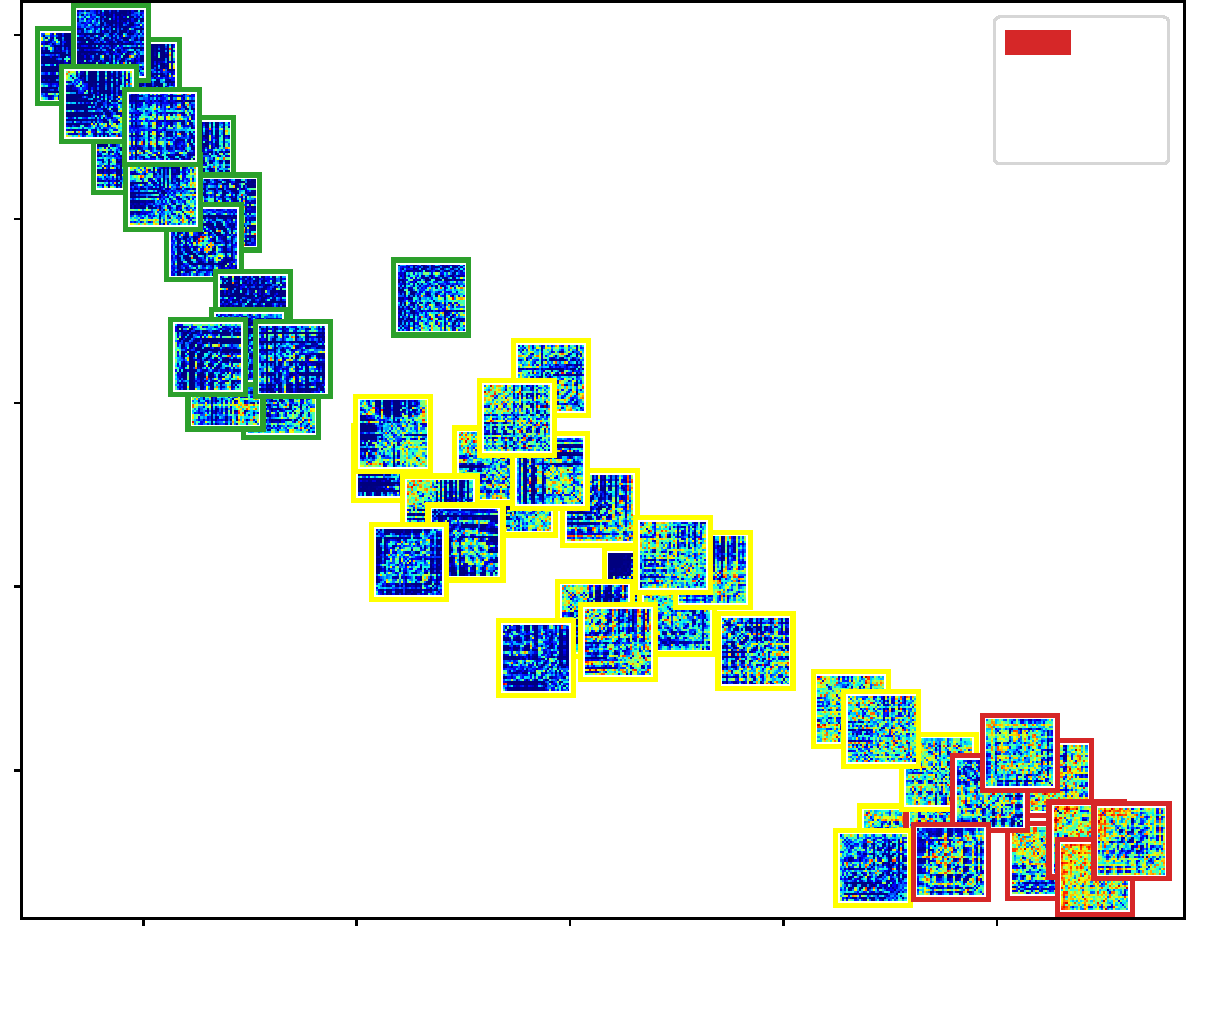
\includegraphics[width=\unitlength,page=1]{../Tesis_document/Figures/Objective_2/pvalue-matrix_2.pdf}}%
    \put(0.90737781,0.7925477){\color[rgb]{0,0,0}\makebox(0,0)[lt]{\lineheight{1.25}\smash{\begin{tabular}[t]{l}G.III\end{tabular}}}}%
    \put(0,0){\includegraphics[width=\unitlength,page=2]{../Tesis_document/Figures/Objective_2/pvalue-matrix_2.pdf}}%
    \put(0.90737781,0.75451951){\color[rgb]{0,0,0}\makebox(0,0)[lt]{\lineheight{1.25}\smash{\begin{tabular}[t]{l}G.II\end{tabular}}}}%
    \put(0,0){\includegraphics[width=\unitlength,page=3]{../Tesis_document/Figures/Objective_2/pvalue-matrix_2.pdf}}%
    \put(0.90737781,0.71649134){\color[rgb]{0,0,0}\makebox(0,0)[lt]{\lineheight{1.25}\smash{\begin{tabular}[t]{l}G.I\end{tabular}}}}%
    \put(0,0){\includegraphics[width=\unitlength,page=4]{../Tesis_document/Figures/Objective_2/pvalue-matrix_2.pdf}}%
    \put(-0.00115551,0.00028681){\color[rgb]{0,0,0}\makebox(0,0)[lt]{\lineheight{1.25}\smash{\begin{tabular}[t]{l}0.00\end{tabular}}}}%
    \put(0,0){\includegraphics[width=\unitlength,page=5]{../Tesis_document/Figures/Objective_2/pvalue-matrix_2.pdf}}%
    \put(0.0470369,0.00028681){\color[rgb]{0,0,0}\makebox(0,0)[lt]{\lineheight{1.25}\smash{\begin{tabular}[t]{l}0.05\end{tabular}}}}%
    \put(0,0){\includegraphics[width=\unitlength,page=6]{../Tesis_document/Figures/Objective_2/pvalue-matrix_2.pdf}}%
    \put(0.09522932,0.00028681){\color[rgb]{0,0,0}\makebox(0,0)[lt]{\lineheight{1.25}\smash{\begin{tabular}[t]{l}0.10\end{tabular}}}}%
    \put(0,0){\includegraphics[width=\unitlength,page=7]{../Tesis_document/Figures/Objective_2/pvalue-matrix_2.pdf}}%
    \put(0.19161414,0.00028681){\color[rgb]{0,0,0}\makebox(0,0)[lt]{\lineheight{1.25}\smash{\begin{tabular}[t]{l}0.20\end{tabular}}}}%
    \put(0,0){\includegraphics[width=\unitlength,page=8]{../Tesis_document/Figures/Objective_2/pvalue-matrix_2.pdf}}%
    \put(0.28799897,0.00028681){\color[rgb]{0,0,0}\makebox(0,0)[lt]{\lineheight{1.25}\smash{\begin{tabular}[t]{l}0.30\end{tabular}}}}%
    \put(0,0){\includegraphics[width=\unitlength,page=9]{../Tesis_document/Figures/Objective_2/pvalue-matrix_2.pdf}}%
    \put(0.38438379,0.00028681){\color[rgb]{0,0,0}\makebox(0,0)[lt]{\lineheight{1.25}\smash{\begin{tabular}[t]{l}0.40\end{tabular}}}}%
    \put(0,0){\includegraphics[width=\unitlength,page=10]{../Tesis_document/Figures/Objective_2/pvalue-matrix_2.pdf}}%
    \put(0.48076862,0.00028681){\color[rgb]{0,0,0}\makebox(0,0)[lt]{\lineheight{1.25}\smash{\begin{tabular}[t]{l}0.50\end{tabular}}}}%
    \put(0,0){\includegraphics[width=\unitlength,page=11]{../Tesis_document/Figures/Objective_2/pvalue-matrix_2.pdf}}%
    \put(0.57715344,0.00028681){\color[rgb]{0,0,0}\makebox(0,0)[lt]{\lineheight{1.25}\smash{\begin{tabular}[t]{l}0.60\end{tabular}}}}%
    \put(0,0){\includegraphics[width=\unitlength,page=12]{../Tesis_document/Figures/Objective_2/pvalue-matrix_2.pdf}}%
    \put(0.67353827,0.00028681){\color[rgb]{0,0,0}\makebox(0,0)[lt]{\lineheight{1.25}\smash{\begin{tabular}[t]{l}0.70\end{tabular}}}}%
    \put(0,0){\includegraphics[width=\unitlength,page=13]{../Tesis_document/Figures/Objective_2/pvalue-matrix_2.pdf}}%
    \put(0.7699231,0.00028681){\color[rgb]{0,0,0}\makebox(0,0)[lt]{\lineheight{1.25}\smash{\begin{tabular}[t]{l}0.80\end{tabular}}}}%
    \put(0,0){\includegraphics[width=\unitlength,page=14]{../Tesis_document/Figures/Objective_2/pvalue-matrix_2.pdf}}%
    \put(0.86630792,0.00028681){\color[rgb]{0,0,0}\makebox(0,0)[lt]{\lineheight{1.25}\smash{\begin{tabular}[t]{l}0.90\end{tabular}}}}%
    \put(0,0){\includegraphics[width=\unitlength,page=15]{../Tesis_document/Figures/Objective_2/pvalue-matrix_2.pdf}}%
    \put(0.96269275,0.00028681){\color[rgb]{0,0,0}\makebox(0,0)[lt]{\lineheight{1.25}\smash{\begin{tabular}[t]{l}1.00\end{tabular}}}}%
    \put(0,0){\includegraphics[width=\unitlength,page=16]{../Tesis_document/Figures/Objective_2/pvalue-matrix_2.pdf}}%
  \end{picture}%
\endgroup%
}
    \caption{
        {{$t$-SNE 2D projection}
            of pruned functional connectivity matrices based on KSC-FCnet and two-sample Kolmogorov--Smirnov test. The color bar depicts the $p$-value of every connection for each subject matrix, where deep blue means more class separability. Therefore, the bluer the matrix, the better the discriminability. Outer boxes indicate subject group belongingness: green G I, yellow G II, and red G III.  $p$-values below $5\%$ are taken as significant.}
    }\label{fig:p-valuematrix}
\end{figure}


%%entropy
\begin{figure}[H]%[h!]
    %\centering
    \resizebox{0.90\linewidth}{!}{% This file was created with tikzplotlib v0.10.1.
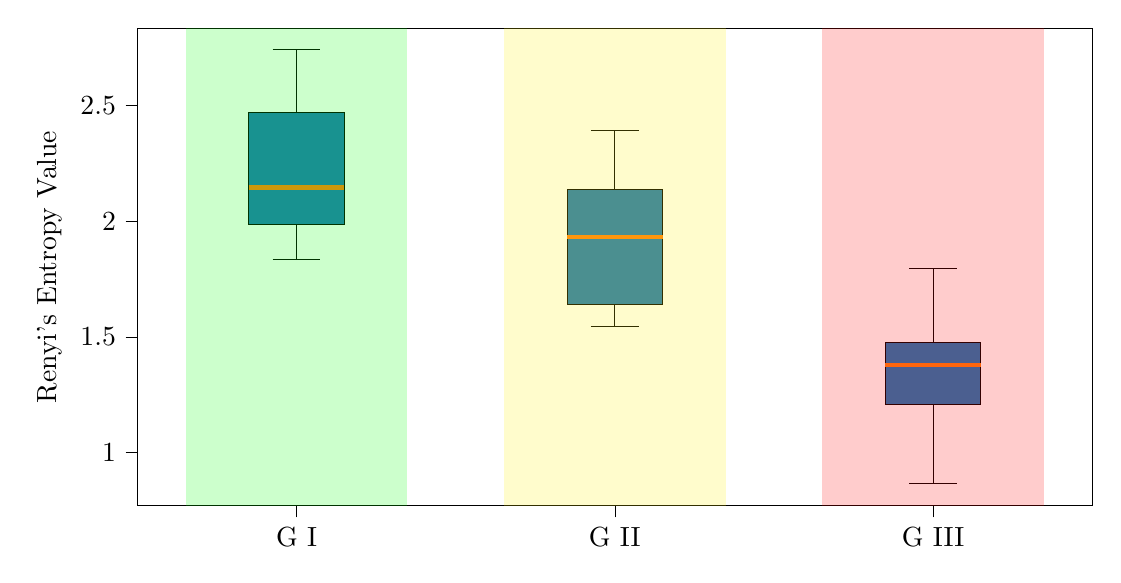
\begin{tikzpicture}

\definecolor{darkgray176}{RGB}{176,176,176}
\definecolor{darkorange25512714}{RGB}{255,127,14}
\definecolor{steelblue31119180}{RGB}{31,119,180}

\begin{axis}[
tick align=outside,
tick pos=left,
x grid style={darkgray176},
xmin=0.5, xmax=3.5,
xtick style={color=black},
y grid style={darkgray176},
ylabel={Renyi's Entropy Value},
ymin=0.770107169384725, ymax=2.83550014961814,
ytick style={color=black},
xtick={1,2,3},
xticklabels={
  G I,
  G II,
  G III
  },
% only scale the axis, not the axis including the ticks and labels
scale only axis=true,
% set `width' and `height' to the desired values
width=\textwidth,
height=0.5\textwidth,
]
\path [draw=black, fill=steelblue31119180]
(axis cs:0.85,1.98710265444379)
--(axis cs:1.15,1.98710265444379)
--(axis cs:1.15,2.4692055467728)
--(axis cs:0.85,2.4692055467728)
--(axis cs:0.85,1.98710265444379)
--cycle;
\addplot [black]
table {%
1 1.98710265444379
1 1.83340962365363
};
\addplot [black]
table {%
1 2.4692055467728
1 2.74161865051662
};
\addplot [black]
table {%
0.925 1.83340962365363
1.075 1.83340962365363
};
\addplot [black]
table {%
0.925 2.74161865051662
1.075 2.74161865051662
};
\path [draw=black, fill=steelblue31119180]
(axis cs:1.85,1.64091629667123)
--(axis cs:2.15,1.64091629667123)
--(axis cs:2.15,2.13763307187243)
--(axis cs:1.85,2.13763307187243)
--(axis cs:1.85,1.64091629667123)
--cycle;
\addplot [black]
table {%
2 1.64091629667123
2 1.54325014822209
};
\addplot [black]
table {%
2 2.13763307187243
2 2.39465148485741
};
\addplot [black]
table {%
1.925 1.54325014822209
2.075 1.54325014822209
};
\addplot [black]
table {%
1.925 2.39465148485741
2.075 2.39465148485741
};
\path [draw=black, fill=steelblue31119180]
(axis cs:2.85,1.20701646656938)
--(axis cs:3.15,1.20701646656938)
--(axis cs:3.15,1.47736138105042)
--(axis cs:2.85,1.47736138105042)
--(axis cs:2.85,1.20701646656938)
--cycle;
\addplot [black]
table {%
3 1.20701646656938
3 0.863988668486244
};
\addplot [black]
table {%
3 1.47736138105042
3 1.7973903501163
};
\addplot [black]
table {%
2.925 0.863988668486244
3.075 0.863988668486244
};
\addplot [black]
table {%
2.925 1.7973903501163
3.075 1.7973903501163
};
\addplot [ultra thick, darkorange25512714]
table {%
0.85 2.14641792100428
1.15 2.14641792100428
};
\addplot [ultra thick, darkorange25512714]
table {%
1.85 1.93151078195408
2.15 1.93151078195408
};
\addplot [ultra thick, darkorange25512714]
table {%
2.85 1.3773748804191
3.15 1.3773748804191
};

\path [draw=green, opacity=0.2, line width=80pt]
(axis cs:1,0.1)
--(axis cs:1,3);

\path [draw=yellow, opacity=0.2, line width=80pt]
(axis cs:2,0.1)
--(axis cs:2,3);

\path [draw=red, opacity=0.2, line width=80pt]
(axis cs:3,0.1)
--(axis cs:3,3);


\end{axis}

\end{tikzpicture}
}
    \caption{Rényi's entropy-based retained information within the estimated functional connectivity matrices using KSC-FCnet. The background codes the group membership (best, medium, and worst performance clusters). Boxplot representation is used to present the retained information within each group.}\label{fig:renyipvalue}
\end{figure}


Further, the Circos plot is a valuable tool to visualize which EEG channels are most important for each subject's experiment. Figure \ref{fig:topoplot_graphs} shows that relevant channel dependencies are kept mainly for the best performance group. Note that all connections are normalized between the three subjects (connectivities above the 99th percentile are shown). For the G I case, the most robust connections are found between the frontal, central left, and right areas, with a few connections in the posterior region. This pattern is consistent with a good-performing subject who presents the most relevant information in the sensorimotor area (central left and right).
Conversely, G II shows significant connections between the center-right and frontal areas, with fewer robust connections in the central left. It is worth noting that EEG noise may be present in the connectivity feature map around the central left region. Notably, G III has no significant connections, indicating that the model could not extract noise-free and discriminative connectivities.

The second and third rows in Figure \ref{fig:topoplot_graphs} depict the most significant brain areas using 2KS and the weights of the last layer in the KCS-FCnet. In G I, similar results are observed, highlighting the sensorimotor area; however, the results in the third row are more concentrated around C4 and C3. It suggests that subjects in the best-performing group do not exhibit much noise and the MI task can be completed using only a few sensors. For G II, there is a slight difference between the results. In particular, a high activation in the left frontal area is observed, while the information is more focused on the sensorimotor area. Finally, for the last group, the most significant difference is observed. While in the 2KS test, some importance (below 0.4) is observed around C4 and C3, in the weight-based approach, there is no clear pattern, indicating that our DL approach can not find relevant information in the sensorimotor area. 


% %% Connectivity
\begin{figure}
     \centering
    \begin{subfigure}[b]{.3\linewidth}
        \centering
        \resizebox{1\linewidth}{!}{%% Creator: Inkscape 1.2.2 (b0a8486541, 2022-12-01), www.inkscape.org
%% PDF/EPS/PS + LaTeX output extension by Johan Engelen, 2010
%% Accompanies image file 'goood.pdf' (pdf, eps, ps)
%%
%% To include the image in your LaTeX document, write
%%   \input{<filename>.pdf_tex}
%%  instead of
%%   \includegraphics{<filename>.pdf}
%% To scale the image, write
%%   \def\svgwidth{<desired width>}
%%   \input{<filename>.pdf_tex}
%%  instead of
%%   \includegraphics[width=<desired width>]{<filename>.pdf}
%%
%% Images with a different path to the parent latex file can
%% be accessed with the `import' package (which may need to be
%% installed) using
%%   \usepackage{import}
%% in the preamble, and then including the image with
%%   \import{<path to file>}{<filename>.pdf_tex}
%% Alternatively, one can specify
%%   \graphicspath{{<path to file>/}}
%% 
%% For more information, please see info/svg-inkscape on CTAN:
%%   http://tug.ctan.org/tex-archive/info/svg-inkscape
%%
\begingroup%
  \makeatletter%
  \providecommand\color[2][]{%
    \errmessage{(Inkscape) Color is used for the text in Inkscape, but the package 'color.sty' is not loaded}%
    \renewcommand\color[2][]{}%
  }%
  \providecommand\transparent[1]{%
    \errmessage{(Inkscape) Transparency is used (non-zero) for the text in Inkscape, but the package 'transparent.sty' is not loaded}%
    \renewcommand\transparent[1]{}%
  }%
  \providecommand\rotatebox[2]{#2}%
  \newcommand*\fsize{\dimexpr\f@size pt\relax}%
  \newcommand*\lineheight[1]{\fontsize{\fsize}{#1\fsize}\selectfont}%
  \ifx\svgwidth\undefined%
    \setlength{\unitlength}{719.99997449bp}%
    \ifx\svgscale\undefined%
      \relax%
    \else%
      \setlength{\unitlength}{\unitlength * \real{\svgscale}}%
    \fi%
  \else%
    \setlength{\unitlength}{\svgwidth}%
  \fi%
  \global\let\svgwidth\undefined%
  \global\let\svgscale\undefined%
  \makeatother%
  \begin{picture}(1,1.00000004)%
    \lineheight{1}%
    \setlength\tabcolsep{0pt}%
    \put(0,0){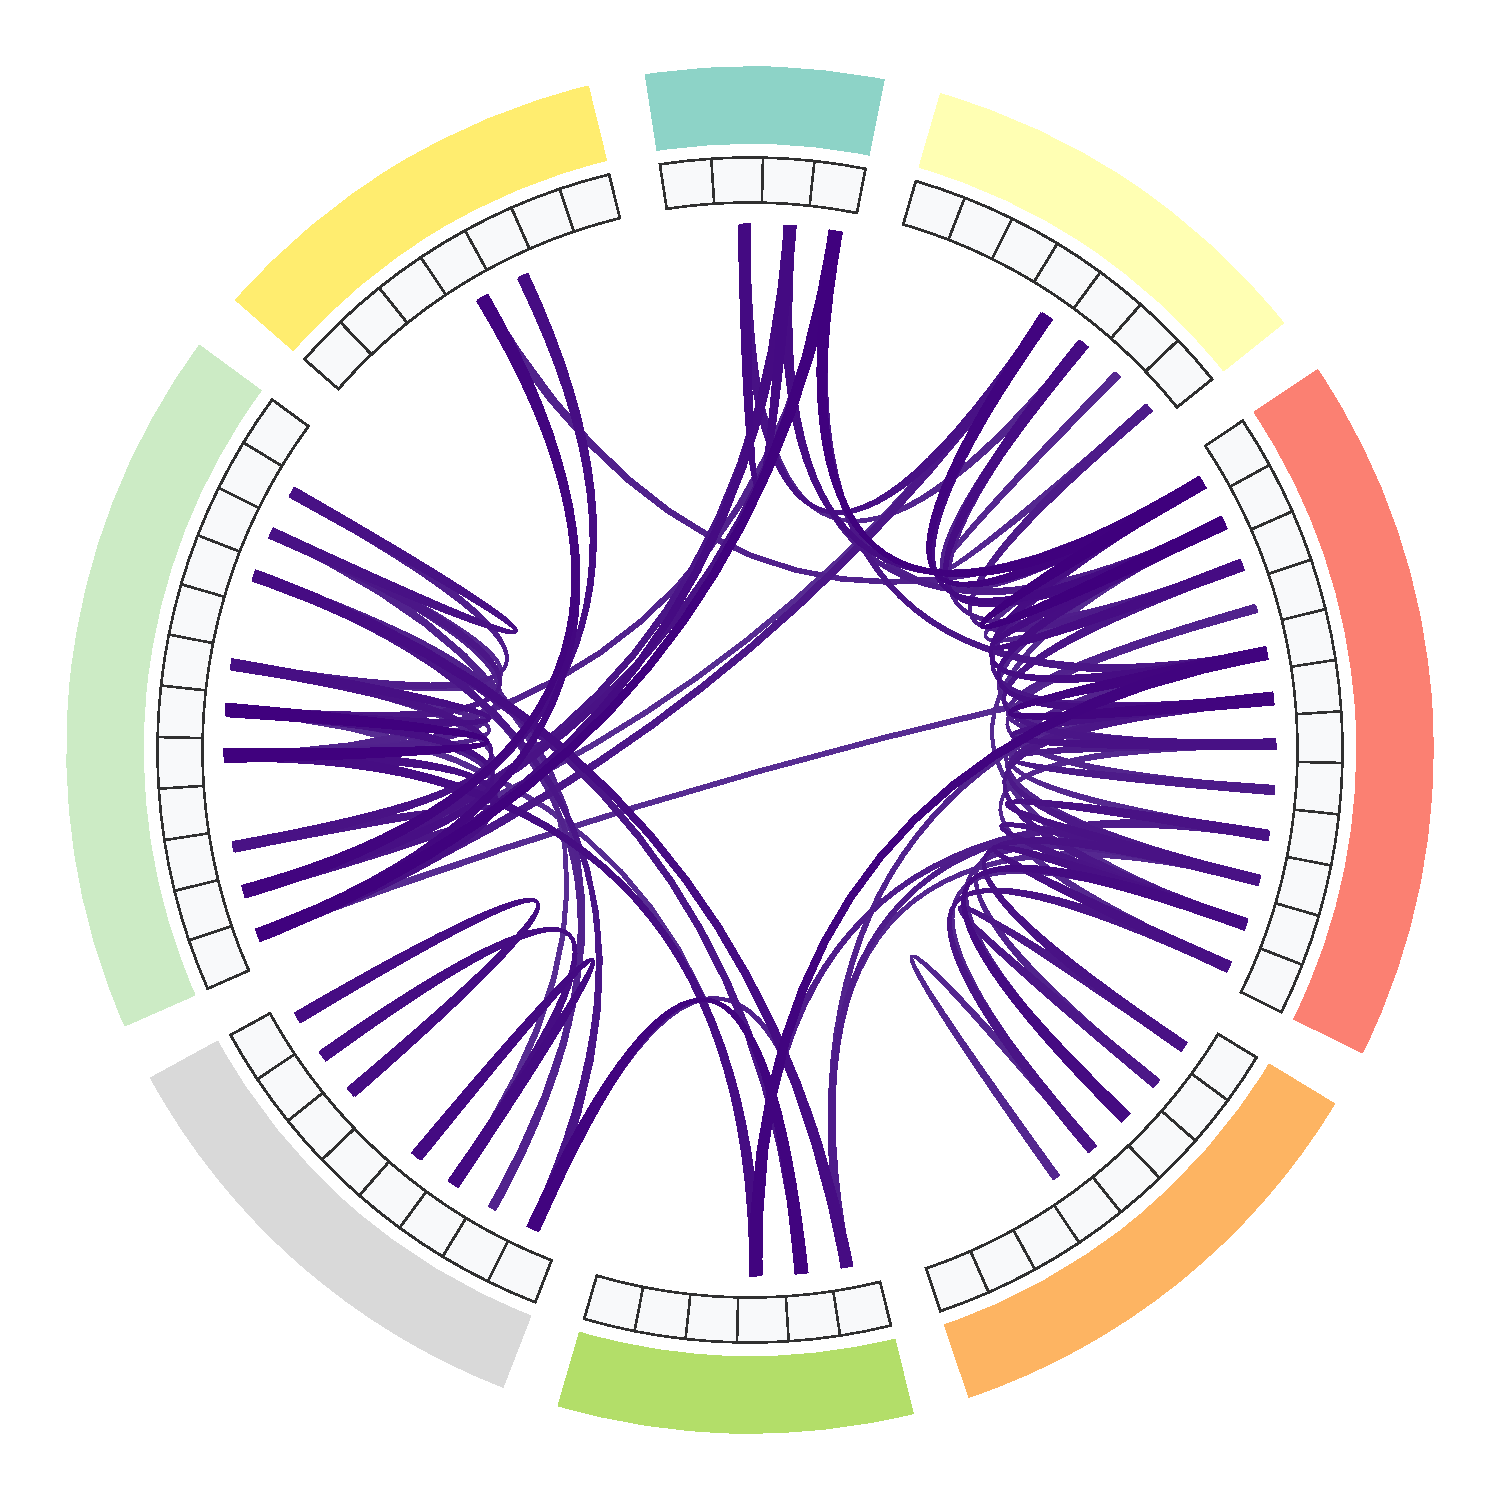
\includegraphics[width=\unitlength,page=1]{Figures/Objective_2/circonnecitvity_good_2.pdf}}%
    \put(0.46180678,0.92326249){\color[rgb]{0,0,0}\rotatebox{-1.25000007}{\makebox(0,0)[lt]{\lineheight{1.25}\smash{\begin{tabular}[t]{l} \LARGE Frontal\end{tabular}}}}}%
    \put(0.66112171,0.90027214){\color[rgb]{0,0,0}\rotatebox{-33.7500015}{\makebox(0,0)[lt]{\lineheight{1.25}\smash{\begin{tabular}[t]{l} \LARGE Frontal Right\end{tabular}}}}}%
    \put(0.91543541,0.61899459){\color[rgb]{0,0,0}\rotatebox{-86.25000021}{\makebox(0,0)[lt]{\lineheight{1.25}\smash{\begin{tabular}[t]{l} \LARGE Central Right\end{tabular}}}}}%
    \put(0.69412406,0.09460069){\color[rgb]{0,0,0}\rotatebox{38.75000159}{\makebox(0,0)[lt]{\lineheight{1.25}\smash{\begin{tabular}[t]{l} \LARGE Posterior Right\end{tabular}}}}}%
    \put(0.42910617,0.06377129){\color[rgb]{0,0,0}\rotatebox{-1.25000007}{\makebox(0,0)[lt]{\lineheight{1.25}\smash{\begin{tabular}[t]{l} \LARGE Posterior\end{tabular}}}}}%
    \put(0.14234136,0.23152432){\color[rgb]{0,0,0}\rotatebox{-41.25000161}{\makebox(0,0)[lt]{\lineheight{1.25}\smash{\begin{tabular}[t]{l} \LARGE Posterior Left\end{tabular}}}}}%
    \put(0.07135272,0.46536155){\color[rgb]{0,0,0}\rotatebox{83.75000035}{\makebox(0,0)[lt]{\lineheight{1.25}\smash{\begin{tabular}[t]{l} \LARGE Central Left\end{tabular}}}}}%
    \put(0.21427494,0.82062027){\color[rgb]{0,0,0}\rotatebox{31.25000144}{\makebox(0,0)[lt]{\lineheight{1.25}\smash{\begin{tabular}[t]{l} \LARGE Frontal Left\end{tabular}}}}}%
    \put(0.43605392,0.8625217){\color[rgb]{0,0,0}\rotatebox{6.25000035}{\makebox(0,0)[lt]{\lineheight{1.25}\smash{\begin{tabular}[t]{l} \LARGE Fpz\end{tabular}}}}}%
    \put(0.46720968,0.86670054){\color[rgb]{0,0,0}\rotatebox{1.25000007}{\makebox(0,0)[lt]{\lineheight{1.25}\smash{\begin{tabular}[t]{l} \LARGE AFz\end{tabular}}}}}%
    \put(0.50877937,0.86754133){\color[rgb]{0,0,0}\rotatebox{-3.75000021}{\makebox(0,0)[lt]{\lineheight{1.25}\smash{\begin{tabular}[t]{l} \LARGE Fz\end{tabular}}}}}%
    \put(0.53119168,0.86685322){\color[rgb]{0,0,0}\rotatebox{-8.75000049}{\makebox(0,0)[lt]{\lineheight{1.25}\smash{\begin{tabular}[t]{l} \LARGE FCz\end{tabular}}}}}%
    \put(0.59379441,0.85607626){\color[rgb]{0,0,0}\rotatebox{-18.75000099}{\makebox(0,0)[lt]{\lineheight{1.25}\smash{\begin{tabular}[t]{l} \LARGE Fp2\end{tabular}}}}}%
    \put(0.6238459,0.84682192){\color[rgb]{0,0,0}\rotatebox{-23.7500012}{\makebox(0,0)[lt]{\lineheight{1.25}\smash{\begin{tabular}[t]{l} \LARGE AF4\end{tabular}}}}}%
    \put(0.65360213,0.83470826){\color[rgb]{0,0,0}\rotatebox{-28.75000137}{\makebox(0,0)[lt]{\lineheight{1.25}\smash{\begin{tabular}[t]{l} \LARGE AF8\end{tabular}}}}}%
    \put(0.69009268,0.8147665){\color[rgb]{0,0,0}\rotatebox{-33.7500015}{\makebox(0,0)[lt]{\lineheight{1.25}\smash{\begin{tabular}[t]{l} \LARGE F2\end{tabular}}}}}%
    \put(0.71680301,0.79700102){\color[rgb]{0,0,0}\rotatebox{-38.75000159}{\makebox(0,0)[lt]{\lineheight{1.25}\smash{\begin{tabular}[t]{l} \LARGE F4\end{tabular}}}}}%
    \put(0.74186335,0.77697521){\color[rgb]{0,0,0}\rotatebox{-43.75000162}{\makebox(0,0)[lt]{\lineheight{1.25}\smash{\begin{tabular}[t]{l} \LARGE F6\end{tabular}}}}}%
    \put(0.76508297,0.75484145){\color[rgb]{0,0,0}\rotatebox{-48.75000161}{\makebox(0,0)[lt]{\lineheight{1.25}\smash{\begin{tabular}[t]{l} \LARGE F8\end{tabular}}}}}%
    \put(0.80027614,0.71323175){\color[rgb]{0,0,0}\rotatebox{-58.75000144}{\makebox(0,0)[lt]{\lineheight{1.25}\smash{\begin{tabular}[t]{l} \LARGE FC2\end{tabular}}}}}%
    \put(0.81771786,0.68624956){\color[rgb]{0,0,0}\rotatebox{-63.75000129}{\makebox(0,0)[lt]{\lineheight{1.25}\smash{\begin{tabular}[t]{l} \LARGE FC4\end{tabular}}}}}%
    \put(0.83274157,0.65784988){\color[rgb]{0,0,0}\rotatebox{-68.7500011}{\makebox(0,0)[lt]{\lineheight{1.25}\smash{\begin{tabular}[t]{l} \LARGE FC6\end{tabular}}}}}%
    \put(0.84564585,0.62683212){\color[rgb]{0,0,0}\rotatebox{-73.75000087}{\makebox(0,0)[lt]{\lineheight{1.25}\smash{\begin{tabular}[t]{l} \LARGE FT8\end{tabular}}}}}%
    \put(0.85665482,0.58983915){\color[rgb]{0,0,0}\rotatebox{-78.75000062}{\makebox(0,0)[lt]{\lineheight{1.25}\smash{\begin{tabular}[t]{l} \LARGE C2\end{tabular}}}}}%
    \put(0.86312764,0.55841276){\color[rgb]{0,0,0}\rotatebox{-83.75000035}{\makebox(0,0)[lt]{\lineheight{1.25}\smash{\begin{tabular}[t]{l} \LARGE C4\end{tabular}}}}}%
    \put(0.86683684,0.52654182){\color[rgb]{0,0,0}\rotatebox{-88.75000007}{\makebox(0,0)[lt]{\lineheight{1.25}\smash{\begin{tabular}[t]{l} \LARGE C6\end{tabular}}}}}%
    \put(0.8676747,0.49325621){\color[rgb]{0,0,0}\rotatebox{-93.74999979}{\makebox(0,0)[lt]{\lineheight{1.25}\smash{\begin{tabular}[t]{l} \LARGE T8\end{tabular}}}}}%
    \put(0.867147,0.47071729){\color[rgb]{0,0,0}\rotatebox{-98.74999951}{\makebox(0,0)[lt]{\lineheight{1.25}\smash{\begin{tabular}[t]{l} \LARGE CP2\end{tabular}}}}}%
    \put(0.86319773,0.43882974){\color[rgb]{0,0,0}\rotatebox{-103.74999925}{\makebox(0,0)[lt]{\lineheight{1.25}\smash{\begin{tabular}[t]{l} \LARGE CP4\end{tabular}}}}}%
    \put(0.85648432,0.40740775){\color[rgb]{0,0,0}\rotatebox{-108.74999901}{\makebox(0,0)[lt]{\lineheight{1.25}\smash{\begin{tabular}[t]{l} \LARGE CP6\end{tabular}}}}}%
    \put(0.84656839,0.37557808){\color[rgb]{0,0,0}\rotatebox{-113.7499988}{\makebox(0,0)[lt]{\lineheight{1.25}\smash{\begin{tabular}[t]{l} \LARGE TP8\end{tabular}}}}}%
    \put(0.81498344,0.31023213){\color[rgb]{0,0,0}\rotatebox{-123.7499985}{\makebox(0,0)[lt]{\lineheight{1.25}\smash{\begin{tabular}[t]{l} \LARGE P2\end{tabular}}}}}%
    \put(0.79724547,0.28350163){\color[rgb]{0,0,0}\rotatebox{-128.74999841}{\makebox(0,0)[lt]{\lineheight{1.25}\smash{\begin{tabular}[t]{l} \LARGE P4\end{tabular}}}}}%
    \put(0.77724528,0.25841882){\color[rgb]{0,0,0}\rotatebox{-133.74999838}{\makebox(0,0)[lt]{\lineheight{1.25}\smash{\begin{tabular}[t]{l} \LARGE P6\end{tabular}}}}}%
    \put(0.7551351,0.23517459){\color[rgb]{0,0,0}\rotatebox{-138.74999839}{\makebox(0,0)[lt]{\lineheight{1.25}\smash{\begin{tabular}[t]{l} \LARGE P8\end{tabular}}}}}%
    \put(0.73820608,0.21916857){\color[rgb]{0,0,0}\rotatebox{-143.74999845}{\makebox(0,0)[lt]{\lineheight{1.25}\smash{\begin{tabular}[t]{l} \LARGE P10\end{tabular}}}}}%
    \put(0.71462318,0.20056822){\color[rgb]{0,0,0}\rotatebox{-148.74999856}{\makebox(0,0)[lt]{\lineheight{1.25}\smash{\begin{tabular}[t]{l} \LARGE PO4\end{tabular}}}}}%
    \put(0.68770927,0.183002){\color[rgb]{0,0,0}\rotatebox{-153.74999871}{\makebox(0,0)[lt]{\lineheight{1.25}\smash{\begin{tabular}[t]{l} \LARGE PO8\end{tabular}}}}}%
    \put(0.65155961,0.16481229){\color[rgb]{0,0,0}\rotatebox{-158.7499989}{\makebox(0,0)[lt]{\lineheight{1.25}\smash{\begin{tabular}[t]{l} \LARGE O2\end{tabular}}}}}%
    \put(0.59654371,0.14467879){\color[rgb]{0,0,0}\rotatebox{-168.74999938}{\makebox(0,0)[lt]{\lineheight{1.25}\smash{\begin{tabular}[t]{l} \LARGE CPz\end{tabular}}}}}%
    \put(0.55556518,0.13656049){\color[rgb]{0,0,0}\rotatebox{-173.74999965}{\makebox(0,0)[lt]{\lineheight{1.25}\smash{\begin{tabular}[t]{l} \LARGE Pz\end{tabular}}}}}%
    \put(0.52500136,0.13312954){\color[rgb]{0,0,0}\rotatebox{-178.74999993}{\makebox(0,0)[lt]{\lineheight{1.25}\smash{\begin{tabular}[t]{l} \LARGE Cz\end{tabular}}}}}%
    \put(0.50252449,0.13171782){\color[rgb]{0,0,0}\rotatebox{176.24999979}{\makebox(0,0)[lt]{\lineheight{1.25}\smash{\begin{tabular}[t]{l} \LARGE POz\end{tabular}}}}}%
    \put(0.46213775,0.13417351){\color[rgb]{0,0,0}\rotatebox{171.24999951}{\makebox(0,0)[lt]{\lineheight{1.25}\smash{\begin{tabular}[t]{l} \LARGE Oz\end{tabular}}}}}%
    \put(0.42375791,0.14049031){\color[rgb]{0,0,0}\rotatebox{166.24999925}{\makebox(0,0)[lt]{\lineheight{1.25}\smash{\begin{tabular}[t]{l} \LARGE Iz\end{tabular}}}}}%
    \put(0.3678114,0.15684901){\color[rgb]{0,0,0}\rotatebox{156.2499988}{\makebox(0,0)[lt]{\lineheight{1.25}\smash{\begin{tabular}[t]{l} \LARGE P1\end{tabular}}}}}%
    \put(0.33840684,0.1696758){\color[rgb]{0,0,0}\rotatebox{151.24999863}{\makebox(0,0)[lt]{\lineheight{1.25}\smash{\begin{tabular}[t]{l} \LARGE P3\end{tabular}}}}}%
    \put(0.31023211,0.18501654){\color[rgb]{0,0,0}\rotatebox{146.2499985}{\makebox(0,0)[lt]{\lineheight{1.25}\smash{\begin{tabular}[t]{l} \LARGE P5\end{tabular}}}}}%
    \put(0.28350162,0.20275452){\color[rgb]{0,0,0}\rotatebox{141.24999841}{\makebox(0,0)[lt]{\lineheight{1.25}\smash{\begin{tabular}[t]{l} \LARGE P7\end{tabular}}}}}%
    \put(0.25841881,0.22275471){\color[rgb]{0,0,0}\rotatebox{136.24999838}{\makebox(0,0)[lt]{\lineheight{1.25}\smash{\begin{tabular}[t]{l} \LARGE P9\end{tabular}}}}}%
    \put(0.24238617,0.23664165){\color[rgb]{0,0,0}\rotatebox{131.24999839}{\makebox(0,0)[lt]{\lineheight{1.25}\smash{\begin{tabular}[t]{l} \LARGE PO3\end{tabular}}}}}%
    \put(0.22041328,0.26009634){\color[rgb]{0,0,0}\rotatebox{126.24999845}{\makebox(0,0)[lt]{\lineheight{1.25}\smash{\begin{tabular}[t]{l} \LARGE PO7\end{tabular}}}}}%
    \put(0.19622259,0.29253821){\color[rgb]{0,0,0}\rotatebox{121.24999856}{\makebox(0,0)[lt]{\lineheight{1.25}\smash{\begin{tabular}[t]{l} \LARGE O1\end{tabular}}}}}%
    \put(0.16725842,0.34215017){\color[rgb]{0,0,0}\rotatebox{111.2499989}{\makebox(0,0)[lt]{\lineheight{1.25}\smash{\begin{tabular}[t]{l} \LARGE FC1\end{tabular}}}}}%
    \put(0.15476708,0.37175117){\color[rgb]{0,0,0}\rotatebox{106.24999913}{\makebox(0,0)[lt]{\lineheight{1.25}\smash{\begin{tabular}[t]{l} \LARGE FC3\end{tabular}}}}}%
    \put(0.14490317,0.40232822){\color[rgb]{0,0,0}\rotatebox{101.24999938}{\makebox(0,0)[lt]{\lineheight{1.25}\smash{\begin{tabular}[t]{l} \LARGE FC5\end{tabular}}}}}%
    \put(0.13758111,0.43511555){\color[rgb]{0,0,0}\rotatebox{96.24999965}{\makebox(0,0)[lt]{\lineheight{1.25}\smash{\begin{tabular}[t]{l} \LARGE FT7\end{tabular}}}}}%
    \put(0.13316316,0.47345821){\color[rgb]{0,0,0}\rotatebox{91.24999993}{\makebox(0,0)[lt]{\lineheight{1.25}\smash{\begin{tabular}[t]{l} \LARGE C1\end{tabular}}}}}%
    \put(0.1322458,0.50553114){\color[rgb]{0,0,0}\rotatebox{86.25000021}{\makebox(0,0)[lt]{\lineheight{1.25}\smash{\begin{tabular}[t]{l} \LARGE C3\end{tabular}}}}}%
    \put(0.13412729,0.537562){\color[rgb]{0,0,0}\rotatebox{81.25000049}{\makebox(0,0)[lt]{\lineheight{1.25}\smash{\begin{tabular}[t]{l} \LARGE C5\end{tabular}}}}}%
    \put(0.13908213,0.57048742){\color[rgb]{0,0,0}\rotatebox{76.25000075}{\makebox(0,0)[lt]{\lineheight{1.25}\smash{\begin{tabular}[t]{l} \LARGE T7\end{tabular}}}}}%
    \put(0.14351567,0.5925923){\color[rgb]{0,0,0}\rotatebox{71.25000099}{\makebox(0,0)[lt]{\lineheight{1.25}\smash{\begin{tabular}[t]{l} \LARGE CP1\end{tabular}}}}}%
    \put(0.15294215,0.62330961){\color[rgb]{0,0,0}\rotatebox{66.2500012}{\makebox(0,0)[lt]{\lineheight{1.25}\smash{\begin{tabular}[t]{l} \LARGE CP3\end{tabular}}}}}%
    \put(0.16500994,0.65308847){\color[rgb]{0,0,0}\rotatebox{61.25000137}{\makebox(0,0)[lt]{\lineheight{1.25}\smash{\begin{tabular}[t]{l} \LARGE CP5\end{tabular}}}}}%
    \put(0.18030239,0.68271269){\color[rgb]{0,0,0}\rotatebox{56.2500015}{\makebox(0,0)[lt]{\lineheight{1.25}\smash{\begin{tabular}[t]{l} \LARGE TP7\end{tabular}}}}}%
    \put(0.21692456,0.73549098){\color[rgb]{0,0,0}\rotatebox{46.25000162}{\makebox(0,0)[lt]{\lineheight{1.25}\smash{\begin{tabular}[t]{l} \LARGE Fp1\end{tabular}}}}}%
    \put(0.23801218,0.75881579){\color[rgb]{0,0,0}\rotatebox{41.25000161}{\makebox(0,0)[lt]{\lineheight{1.25}\smash{\begin{tabular}[t]{l} \LARGE AF3\end{tabular}}}}}%
    \put(0.2615664,0.78066466){\color[rgb]{0,0,0}\rotatebox{36.25000155}{\makebox(0,0)[lt]{\lineheight{1.25}\smash{\begin{tabular}[t]{l} \LARGE AF7\end{tabular}}}}}%
    \put(0.29506136,0.80530855){\color[rgb]{0,0,0}\rotatebox{31.25000144}{\makebox(0,0)[lt]{\lineheight{1.25}\smash{\begin{tabular}[t]{l} \LARGE F1\end{tabular}}}}}%
    \put(0.3224506,0.82200836){\color[rgb]{0,0,0}\rotatebox{26.25000129}{\makebox(0,0)[lt]{\lineheight{1.25}\smash{\begin{tabular}[t]{l} \LARGE F3\end{tabular}}}}}%
    \put(0.3511911,0.83625747){\color[rgb]{0,0,0}\rotatebox{21.2500011}{\makebox(0,0)[lt]{\lineheight{1.25}\smash{\begin{tabular}[t]{l} \LARGE F5\end{tabular}}}}}%
    \put(0.38106413,0.84794743){\color[rgb]{0,0,0}\rotatebox{16.25000087}{\makebox(0,0)[lt]{\lineheight{1.25}\smash{\begin{tabular}[t]{l} \LARGE F7\end{tabular}}}}}%
  \end{picture}%
\endgroup%
}
    \end{subfigure}
    ~
    \begin{subfigure}[b]{.3\linewidth}
        \centering 	\resizebox{1\linewidth}{!}{%% Creator: Inkscape 1.2.2 (b0a8486541, 2022-12-01), www.inkscape.org
%% PDF/EPS/PS + LaTeX output extension by Johan Engelen, 2010
%% Accompanies image file 'circonnecitvity_medium.pdf' (pdf, eps, ps)
%%
%% To include the image in your LaTeX document, write
%%   \input{<filename>.pdf_tex}
%%  instead of
%%   \includegraphics{<filename>.pdf}
%% To scale the image, write
%%   \def\svgwidth{<desired width>}
%%   \input{<filename>.pdf_tex}
%%  instead of
%%   \includegraphics[width=<desired width>]{<filename>.pdf}
%%
%% Images with a different path to the parent latex file can
%% be accessed with the `import' package (which may need to be
%% installed) using
%%   \usepackage{import}
%% in the preamble, and then including the image with
%%   \import{<path to file>}{<filename>.pdf_tex}
%% Alternatively, one can specify
%%   \graphicspath{{<path to file>/}}
%% 
%% For more information, please see info/svg-inkscape on CTAN:
%%   http://tug.ctan.org/tex-archive/info/svg-inkscape
%%
\begingroup%
  \makeatletter%
  \providecommand\color[2][]{%
    \errmessage{(Inkscape) Color is used for the text in Inkscape, but the package 'color.sty' is not loaded}%
    \renewcommand\color[2][]{}%
  }%
  \providecommand\transparent[1]{%
    \errmessage{(Inkscape) Transparency is used (non-zero) for the text in Inkscape, but the package 'transparent.sty' is not loaded}%
    \renewcommand\transparent[1]{}%
  }%
  \providecommand\rotatebox[2]{#2}%
  \newcommand*\fsize{\dimexpr\f@size pt\relax}%
  \newcommand*\lineheight[1]{\fontsize{\fsize}{#1\fsize}\selectfont}%
  \ifx\svgwidth\undefined%
    \setlength{\unitlength}{719.99997732bp}%
    \ifx\svgscale\undefined%
      \relax%
    \else%
      \setlength{\unitlength}{\unitlength * \real{\svgscale}}%
    \fi%
  \else%
    \setlength{\unitlength}{\svgwidth}%
  \fi%
  \global\let\svgwidth\undefined%
  \global\let\svgscale\undefined%
  \makeatother%
  \begin{picture}(1,1.00000004)%
    \lineheight{1}%
    \setlength\tabcolsep{0pt}%
    \put(0,0){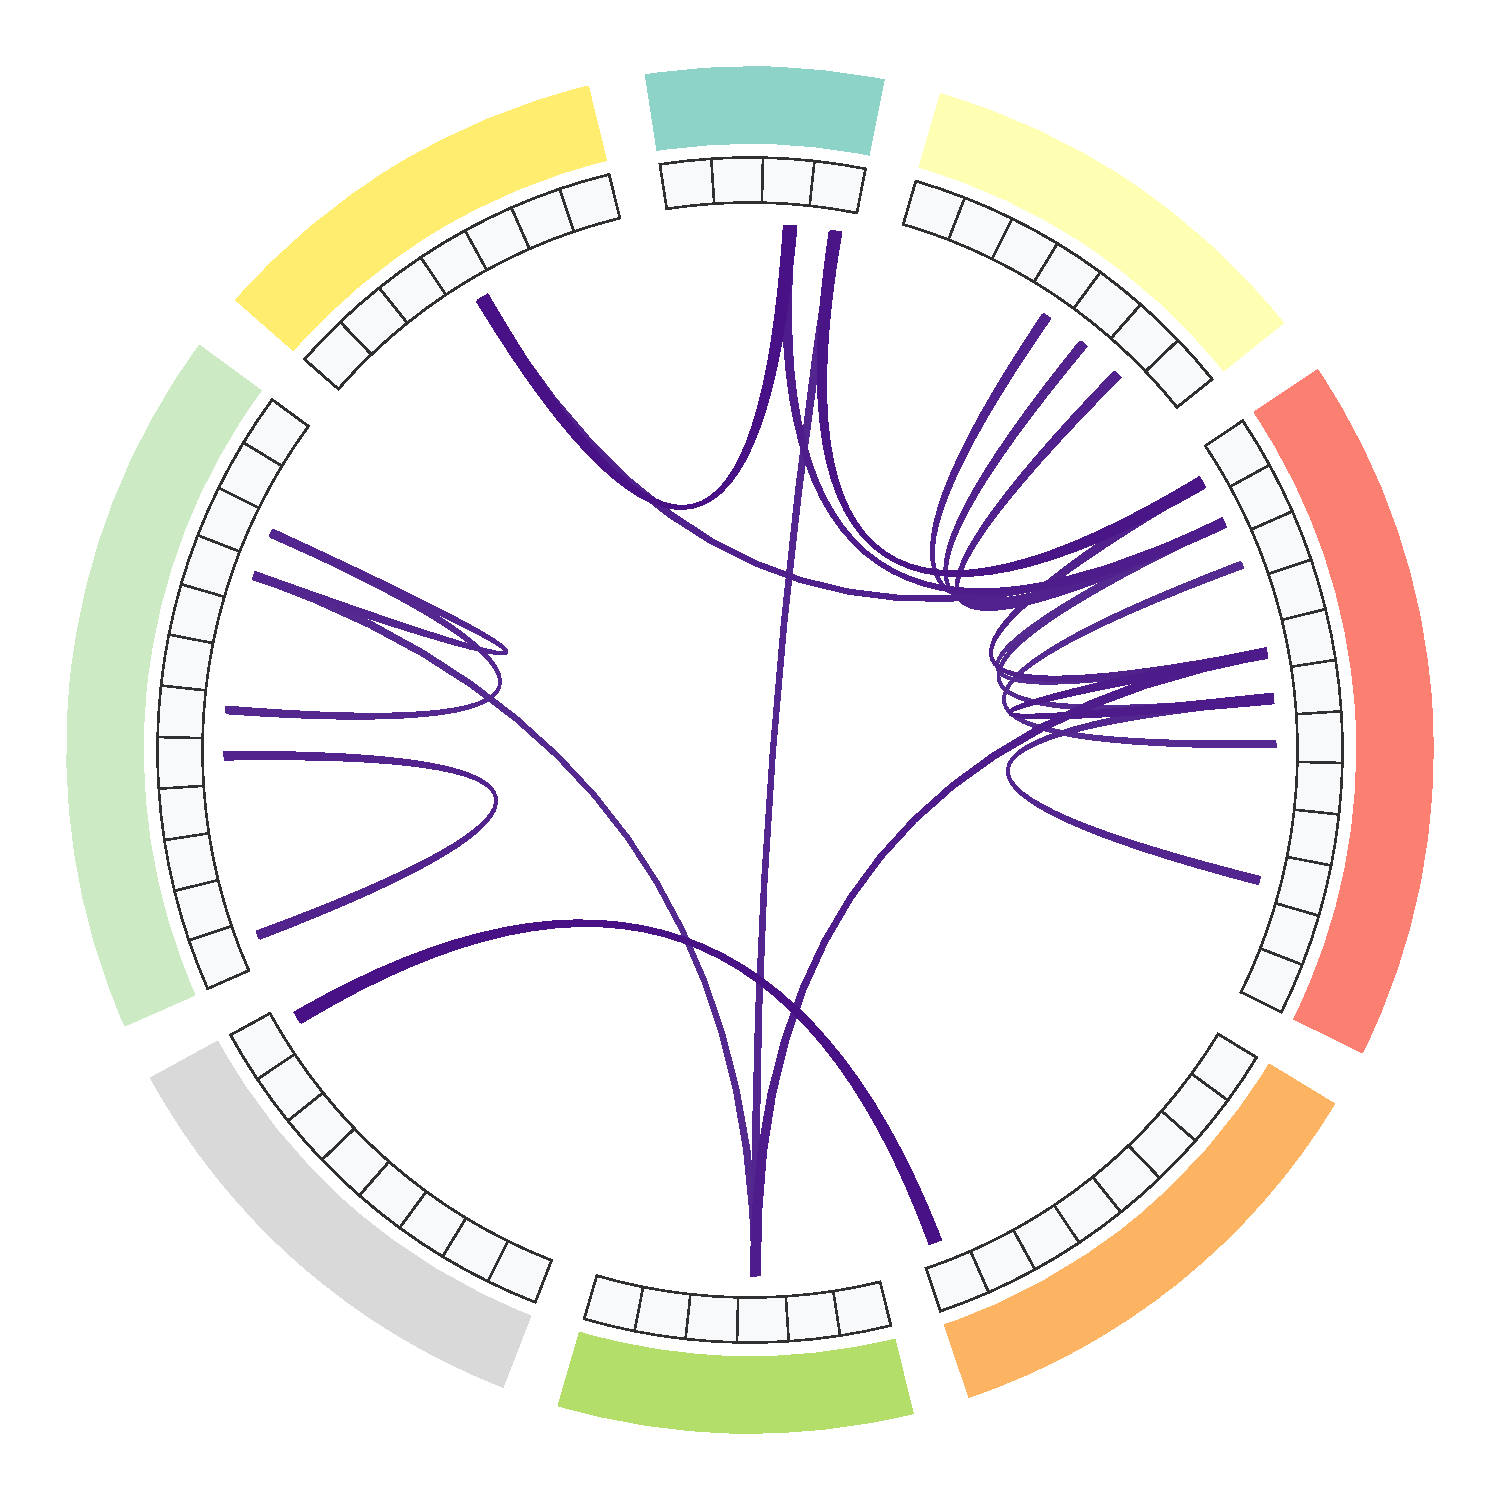
\includegraphics[width=\unitlength,page=1]{../Tesis_document/Figures/Objective_2/circonnecitvity_medium_2.pdf}}%
    \put(0.46180678,0.92326249){\color[rgb]{0,0,0}\rotatebox{-1.25000007}{\makebox(0,0)[lt]{\lineheight{1.25}\smash{\begin{tabular}[t]{l} \LARGE Frontal\end{tabular}}}}}%
    \put(0.66112171,0.90027214){\color[rgb]{0,0,0}\rotatebox{-33.7500015}{\makebox(0,0)[lt]{\lineheight{1.25}\smash{\begin{tabular}[t]{l} \LARGE Frontal Right\end{tabular}}}}}%
    \put(0.91543541,0.61899459){\color[rgb]{0,0,0}\rotatebox{-86.25000021}{\makebox(0,0)[lt]{\lineheight{1.25}\smash{\begin{tabular}[t]{l} \LARGE Central Right\end{tabular}}}}}%
    \put(0.69412405,0.09460069){\color[rgb]{0,0,0}\rotatebox{38.75000159}{\makebox(0,0)[lt]{\lineheight{1.25}\smash{\begin{tabular}[t]{l} \LARGE Posterior Right\end{tabular}}}}}%
    \put(0.42910617,0.06377129){\color[rgb]{0,0,0}\rotatebox{-1.25000007}{\makebox(0,0)[lt]{\lineheight{1.25}\smash{\begin{tabular}[t]{l} \LARGE Posterior\end{tabular}}}}}%
    \put(0.14234136,0.23152432){\color[rgb]{0,0,0}\rotatebox{-41.25000161}{\makebox(0,0)[lt]{\lineheight{1.25}\smash{\begin{tabular}[t]{l} \LARGE Posterior Left\end{tabular}}}}}%
    \put(0.07135272,0.46536154){\color[rgb]{0,0,0}\rotatebox{83.75000035}{\makebox(0,0)[lt]{\lineheight{1.25}\smash{\begin{tabular}[t]{l} \LARGE Central Left\end{tabular}}}}}%
    \put(0.21427494,0.82062026){\color[rgb]{0,0,0}\rotatebox{31.25000144}{\makebox(0,0)[lt]{\lineheight{1.25}\smash{\begin{tabular}[t]{l} \LARGE Frontal Left\end{tabular}}}}}%
    \put(0.43605392,0.86252169){\color[rgb]{0,0,0}\rotatebox{6.25000035}{\makebox(0,0)[lt]{\lineheight{1.25}\smash{\begin{tabular}[t]{l} \LARGE Fpz\end{tabular}}}}}%
    \put(0.46720968,0.86670054){\color[rgb]{0,0,0}\rotatebox{1.25000007}{\makebox(0,0)[lt]{\lineheight{1.25}\smash{\begin{tabular}[t]{l} \LARGE AFz\end{tabular}}}}}%
    \put(0.50877936,0.86754133){\color[rgb]{0,0,0}\rotatebox{-3.75000021}{\makebox(0,0)[lt]{\lineheight{1.25}\smash{\begin{tabular}[t]{l} \LARGE Fz\end{tabular}}}}}%
    \put(0.53119167,0.86685321){\color[rgb]{0,0,0}\rotatebox{-8.75000049}{\makebox(0,0)[lt]{\lineheight{1.25}\smash{\begin{tabular}[t]{l} \LARGE FCz\end{tabular}}}}}%
    \put(0.59379441,0.85607626){\color[rgb]{0,0,0}\rotatebox{-18.75000099}{\makebox(0,0)[lt]{\lineheight{1.25}\smash{\begin{tabular}[t]{l} \LARGE Fp2\end{tabular}}}}}%
    \put(0.62384589,0.84682192){\color[rgb]{0,0,0}\rotatebox{-23.7500012}{\makebox(0,0)[lt]{\lineheight{1.25}\smash{\begin{tabular}[t]{l} \LARGE AF4\end{tabular}}}}}%
    \put(0.65360213,0.83470826){\color[rgb]{0,0,0}\rotatebox{-28.75000137}{\makebox(0,0)[lt]{\lineheight{1.25}\smash{\begin{tabular}[t]{l} \LARGE AF8\end{tabular}}}}}%
    \put(0.69009268,0.8147665){\color[rgb]{0,0,0}\rotatebox{-33.7500015}{\makebox(0,0)[lt]{\lineheight{1.25}\smash{\begin{tabular}[t]{l} \LARGE F2\end{tabular}}}}}%
    \put(0.716803,0.79700101){\color[rgb]{0,0,0}\rotatebox{-38.75000159}{\makebox(0,0)[lt]{\lineheight{1.25}\smash{\begin{tabular}[t]{l} \LARGE F4\end{tabular}}}}}%
    \put(0.74186335,0.77697521){\color[rgb]{0,0,0}\rotatebox{-43.75000162}{\makebox(0,0)[lt]{\lineheight{1.25}\smash{\begin{tabular}[t]{l} \LARGE F6\end{tabular}}}}}%
    \put(0.76508296,0.75484145){\color[rgb]{0,0,0}\rotatebox{-48.75000161}{\makebox(0,0)[lt]{\lineheight{1.25}\smash{\begin{tabular}[t]{l} \LARGE F8\end{tabular}}}}}%
    \put(0.80027613,0.71323175){\color[rgb]{0,0,0}\rotatebox{-58.75000144}{\makebox(0,0)[lt]{\lineheight{1.25}\smash{\begin{tabular}[t]{l} \LARGE FC2\end{tabular}}}}}%
    \put(0.81771786,0.68624956){\color[rgb]{0,0,0}\rotatebox{-63.75000129}{\makebox(0,0)[lt]{\lineheight{1.25}\smash{\begin{tabular}[t]{l} \LARGE FC4\end{tabular}}}}}%
    \put(0.83274156,0.65784988){\color[rgb]{0,0,0}\rotatebox{-68.7500011}{\makebox(0,0)[lt]{\lineheight{1.25}\smash{\begin{tabular}[t]{l} \LARGE FC6\end{tabular}}}}}%
    \put(0.84564584,0.62683212){\color[rgb]{0,0,0}\rotatebox{-73.75000087}{\makebox(0,0)[lt]{\lineheight{1.25}\smash{\begin{tabular}[t]{l} \LARGE FT8\end{tabular}}}}}%
    \put(0.85665482,0.58983915){\color[rgb]{0,0,0}\rotatebox{-78.75000062}{\makebox(0,0)[lt]{\lineheight{1.25}\smash{\begin{tabular}[t]{l} \LARGE C2\end{tabular}}}}}%
    \put(0.86312764,0.55841276){\color[rgb]{0,0,0}\rotatebox{-83.75000035}{\makebox(0,0)[lt]{\lineheight{1.25}\smash{\begin{tabular}[t]{l} \LARGE C4\end{tabular}}}}}%
    \put(0.86683684,0.52654182){\color[rgb]{0,0,0}\rotatebox{-88.75000007}{\makebox(0,0)[lt]{\lineheight{1.25}\smash{\begin{tabular}[t]{l} \LARGE C6\end{tabular}}}}}%
    \put(0.8676747,0.49325621){\color[rgb]{0,0,0}\rotatebox{-93.74999979}{\makebox(0,0)[lt]{\lineheight{1.25}\smash{\begin{tabular}[t]{l} \LARGE T8\end{tabular}}}}}%
    \put(0.867147,0.47071729){\color[rgb]{0,0,0}\rotatebox{-98.74999951}{\makebox(0,0)[lt]{\lineheight{1.25}\smash{\begin{tabular}[t]{l} \LARGE CP2\end{tabular}}}}}%
    \put(0.86319772,0.43882974){\color[rgb]{0,0,0}\rotatebox{-103.74999925}{\makebox(0,0)[lt]{\lineheight{1.25}\smash{\begin{tabular}[t]{l} \LARGE CP4\end{tabular}}}}}%
    \put(0.85648431,0.40740775){\color[rgb]{0,0,0}\rotatebox{-108.74999901}{\makebox(0,0)[lt]{\lineheight{1.25}\smash{\begin{tabular}[t]{l} \LARGE CP6\end{tabular}}}}}%
    \put(0.84656839,0.37557808){\color[rgb]{0,0,0}\rotatebox{-113.7499988}{\makebox(0,0)[lt]{\lineheight{1.25}\smash{\begin{tabular}[t]{l} \LARGE TP8\end{tabular}}}}}%
    \put(0.81498344,0.31023213){\color[rgb]{0,0,0}\rotatebox{-123.7499985}{\makebox(0,0)[lt]{\lineheight{1.25}\smash{\begin{tabular}[t]{l} \LARGE P2\end{tabular}}}}}%
    \put(0.79724547,0.28350163){\color[rgb]{0,0,0}\rotatebox{-128.74999841}{\makebox(0,0)[lt]{\lineheight{1.25}\smash{\begin{tabular}[t]{l} \LARGE P4\end{tabular}}}}}%
    \put(0.77724528,0.25841882){\color[rgb]{0,0,0}\rotatebox{-133.74999838}{\makebox(0,0)[lt]{\lineheight{1.25}\smash{\begin{tabular}[t]{l} \LARGE P6\end{tabular}}}}}%
    \put(0.7551351,0.23517459){\color[rgb]{0,0,0}\rotatebox{-138.74999839}{\makebox(0,0)[lt]{\lineheight{1.25}\smash{\begin{tabular}[t]{l} \LARGE P8\end{tabular}}}}}%
    \put(0.73820608,0.21916856){\color[rgb]{0,0,0}\rotatebox{-143.74999845}{\makebox(0,0)[lt]{\lineheight{1.25}\smash{\begin{tabular}[t]{l} \LARGE P10\end{tabular}}}}}%
    \put(0.71462318,0.20056822){\color[rgb]{0,0,0}\rotatebox{-148.74999856}{\makebox(0,0)[lt]{\lineheight{1.25}\smash{\begin{tabular}[t]{l} \LARGE PO4\end{tabular}}}}}%
    \put(0.68770927,0.183002){\color[rgb]{0,0,0}\rotatebox{-153.74999871}{\makebox(0,0)[lt]{\lineheight{1.25}\smash{\begin{tabular}[t]{l} \LARGE PO8\end{tabular}}}}}%
    \put(0.6515596,0.16481229){\color[rgb]{0,0,0}\rotatebox{-158.7499989}{\makebox(0,0)[lt]{\lineheight{1.25}\smash{\begin{tabular}[t]{l} \LARGE O2\end{tabular}}}}}%
    \put(0.59654371,0.14467879){\color[rgb]{0,0,0}\rotatebox{-168.74999938}{\makebox(0,0)[lt]{\lineheight{1.25}\smash{\begin{tabular}[t]{l} \LARGE CPz\end{tabular}}}}}%
    \put(0.55556518,0.13656049){\color[rgb]{0,0,0}\rotatebox{-173.74999965}{\makebox(0,0)[lt]{\lineheight{1.25}\smash{\begin{tabular}[t]{l} \LARGE Pz\end{tabular}}}}}%
    \put(0.52500135,0.13312954){\color[rgb]{0,0,0}\rotatebox{-178.74999993}{\makebox(0,0)[lt]{\lineheight{1.25}\smash{\begin{tabular}[t]{l} \LARGE Cz\end{tabular}}}}}%
    \put(0.50252449,0.13171781){\color[rgb]{0,0,0}\rotatebox{176.24999979}{\makebox(0,0)[lt]{\lineheight{1.25}\smash{\begin{tabular}[t]{l} \LARGE POz\end{tabular}}}}}%
    \put(0.46213775,0.13417351){\color[rgb]{0,0,0}\rotatebox{171.24999951}{\makebox(0,0)[lt]{\lineheight{1.25}\smash{\begin{tabular}[t]{l} \LARGE Oz\end{tabular}}}}}%
    \put(0.42375791,0.14049031){\color[rgb]{0,0,0}\rotatebox{166.24999925}{\makebox(0,0)[lt]{\lineheight{1.25}\smash{\begin{tabular}[t]{l} \LARGE Iz\end{tabular}}}}}%
    \put(0.3678114,0.15684901){\color[rgb]{0,0,0}\rotatebox{156.2499988}{\makebox(0,0)[lt]{\lineheight{1.25}\smash{\begin{tabular}[t]{l} \LARGE P1\end{tabular}}}}}%
    \put(0.33840684,0.1696758){\color[rgb]{0,0,0}\rotatebox{151.24999863}{\makebox(0,0)[lt]{\lineheight{1.25}\smash{\begin{tabular}[t]{l} \LARGE P3\end{tabular}}}}}%
    \put(0.3102321,0.18501654){\color[rgb]{0,0,0}\rotatebox{146.2499985}{\makebox(0,0)[lt]{\lineheight{1.25}\smash{\begin{tabular}[t]{l} \LARGE P5\end{tabular}}}}}%
    \put(0.28350161,0.20275451){\color[rgb]{0,0,0}\rotatebox{141.24999841}{\makebox(0,0)[lt]{\lineheight{1.25}\smash{\begin{tabular}[t]{l} \LARGE P7\end{tabular}}}}}%
    \put(0.25841881,0.22275471){\color[rgb]{0,0,0}\rotatebox{136.24999838}{\makebox(0,0)[lt]{\lineheight{1.25}\smash{\begin{tabular}[t]{l} \LARGE P9\end{tabular}}}}}%
    \put(0.24238617,0.23664165){\color[rgb]{0,0,0}\rotatebox{131.24999839}{\makebox(0,0)[lt]{\lineheight{1.25}\smash{\begin{tabular}[t]{l} \LARGE PO3\end{tabular}}}}}%
    \put(0.22041328,0.26009634){\color[rgb]{0,0,0}\rotatebox{126.24999845}{\makebox(0,0)[lt]{\lineheight{1.25}\smash{\begin{tabular}[t]{l} \LARGE PO7\end{tabular}}}}}%
    \put(0.19622258,0.29253821){\color[rgb]{0,0,0}\rotatebox{121.24999856}{\makebox(0,0)[lt]{\lineheight{1.25}\smash{\begin{tabular}[t]{l} \LARGE O1\end{tabular}}}}}%
    \put(0.16725842,0.34215017){\color[rgb]{0,0,0}\rotatebox{111.2499989}{\makebox(0,0)[lt]{\lineheight{1.25}\smash{\begin{tabular}[t]{l} \LARGE FC1\end{tabular}}}}}%
    \put(0.15476708,0.37175117){\color[rgb]{0,0,0}\rotatebox{106.24999913}{\makebox(0,0)[lt]{\lineheight{1.25}\smash{\begin{tabular}[t]{l} \LARGE FC3\end{tabular}}}}}%
    \put(0.14490317,0.40232822){\color[rgb]{0,0,0}\rotatebox{101.24999938}{\makebox(0,0)[lt]{\lineheight{1.25}\smash{\begin{tabular}[t]{l} \LARGE FC5\end{tabular}}}}}%
    \put(0.13758111,0.43511555){\color[rgb]{0,0,0}\rotatebox{96.24999965}{\makebox(0,0)[lt]{\lineheight{1.25}\smash{\begin{tabular}[t]{l} \LARGE FT7\end{tabular}}}}}%
    \put(0.13316316,0.47345821){\color[rgb]{0,0,0}\rotatebox{91.24999993}{\makebox(0,0)[lt]{\lineheight{1.25}\smash{\begin{tabular}[t]{l} \LARGE C1\end{tabular}}}}}%
    \put(0.1322458,0.50553114){\color[rgb]{0,0,0}\rotatebox{86.25000021}{\makebox(0,0)[lt]{\lineheight{1.25}\smash{\begin{tabular}[t]{l} \LARGE C3\end{tabular}}}}}%
    \put(0.13412729,0.537562){\color[rgb]{0,0,0}\rotatebox{81.25000049}{\makebox(0,0)[lt]{\lineheight{1.25}\smash{\begin{tabular}[t]{l} \LARGE C5\end{tabular}}}}}%
    \put(0.13908213,0.57048741){\color[rgb]{0,0,0}\rotatebox{76.25000075}{\makebox(0,0)[lt]{\lineheight{1.25}\smash{\begin{tabular}[t]{l} \LARGE T7\end{tabular}}}}}%
    \put(0.14351567,0.5925923){\color[rgb]{0,0,0}\rotatebox{71.25000099}{\makebox(0,0)[lt]{\lineheight{1.25}\smash{\begin{tabular}[t]{l} \LARGE CP1\end{tabular}}}}}%
    \put(0.15294215,0.62330961){\color[rgb]{0,0,0}\rotatebox{66.2500012}{\makebox(0,0)[lt]{\lineheight{1.25}\smash{\begin{tabular}[t]{l} \LARGE CP3\end{tabular}}}}}%
    \put(0.16500994,0.65308846){\color[rgb]{0,0,0}\rotatebox{61.25000137}{\makebox(0,0)[lt]{\lineheight{1.25}\smash{\begin{tabular}[t]{l} \LARGE CP5\end{tabular}}}}}%
    \put(0.18030239,0.68271269){\color[rgb]{0,0,0}\rotatebox{56.2500015}{\makebox(0,0)[lt]{\lineheight{1.25}\smash{\begin{tabular}[t]{l} \LARGE TP7\end{tabular}}}}}%
    \put(0.21692456,0.73549098){\color[rgb]{0,0,0}\rotatebox{46.25000162}{\makebox(0,0)[lt]{\lineheight{1.25}\smash{\begin{tabular}[t]{l} \LARGE Fp1\end{tabular}}}}}%
    \put(0.23801217,0.75881578){\color[rgb]{0,0,0}\rotatebox{41.25000161}{\makebox(0,0)[lt]{\lineheight{1.25}\smash{\begin{tabular}[t]{l} \LARGE AF3\end{tabular}}}}}%
    \put(0.2615664,0.78066465){\color[rgb]{0,0,0}\rotatebox{36.25000155}{\makebox(0,0)[lt]{\lineheight{1.25}\smash{\begin{tabular}[t]{l} \LARGE AF7\end{tabular}}}}}%
    \put(0.29506136,0.80530855){\color[rgb]{0,0,0}\rotatebox{31.25000144}{\makebox(0,0)[lt]{\lineheight{1.25}\smash{\begin{tabular}[t]{l} \LARGE F1\end{tabular}}}}}%
    \put(0.3224506,0.82200836){\color[rgb]{0,0,0}\rotatebox{26.25000129}{\makebox(0,0)[lt]{\lineheight{1.25}\smash{\begin{tabular}[t]{l} \LARGE F3\end{tabular}}}}}%
    \put(0.3511911,0.83625747){\color[rgb]{0,0,0}\rotatebox{21.2500011}{\makebox(0,0)[lt]{\lineheight{1.25}\smash{\begin{tabular}[t]{l} \LARGE F5\end{tabular}}}}}%
    \put(0.38106413,0.84794742){\color[rgb]{0,0,0}\rotatebox{16.25000087}{\makebox(0,0)[lt]{\lineheight{1.25}\smash{\begin{tabular}[t]{l} \LARGE F7\end{tabular}}}}}%
  \end{picture}%
\endgroup%
}	
    \end{subfigure}
    ~
    \begin{subfigure}[b]{.3\linewidth}
        \centering
        \resizebox{1\linewidth}{!}{%% Creator: Inkscape 1.2.2 (b0a8486541, 2022-12-01), www.inkscape.org
%% PDF/EPS/PS + LaTeX output extension by Johan Engelen, 2010
%% Accompanies image file 'circonnecitvity_bad.pdf' (pdf, eps, ps)
%%
%% To include the image in your LaTeX document, write
%%   \input{<filename>.pdf_tex}
%%  instead of
%%   \includegraphics{<filename>.pdf}
%% To scale the image, write
%%   \def\svgwidth{<desired width>}
%%   \input{<filename>.pdf_tex}
%%  instead of
%%   \includegraphics[width=<desired width>]{<filename>.pdf}
%%
%% Images with a different path to the parent latex file can
%% be accessed with the `import' package (which may need to be
%% installed) using
%%   \usepackage{import}
%% in the preamble, and then including the image with
%%   \import{<path to file>}{<filename>.pdf_tex}
%% Alternatively, one can specify
%%   \graphicspath{{<path to file>/}}
%% 
%% For more information, please see info/svg-inkscape on CTAN:
%%   http://tug.ctan.org/tex-archive/info/svg-inkscape
%%
\begingroup%
  \makeatletter%
  \providecommand\color[2][]{%
    \errmessage{(Inkscape) Color is used for the text in Inkscape, but the package 'color.sty' is not loaded}%
    \renewcommand\color[2][]{}%
  }%
  \providecommand\transparent[1]{%
    \errmessage{(Inkscape) Transparency is used (non-zero) for the text in Inkscape, but the package 'transparent.sty' is not loaded}%
    \renewcommand\transparent[1]{}%
  }%
  \providecommand\rotatebox[2]{#2}%
  \newcommand*\fsize{\dimexpr\f@size pt\relax}%
  \newcommand*\lineheight[1]{\fontsize{\fsize}{#1\fsize}\selectfont}%
  \ifx\svgwidth\undefined%
    \setlength{\unitlength}{719.9999915bp}%
    \ifx\svgscale\undefined%
      \relax%
    \else%
      \setlength{\unitlength}{\unitlength * \real{\svgscale}}%
    \fi%
  \else%
    \setlength{\unitlength}{\svgwidth}%
  \fi%
  \global\let\svgwidth\undefined%
  \global\let\svgscale\undefined%
  \makeatother%
  \begin{picture}(1,1.00000002)%
    \lineheight{1}%
    \setlength\tabcolsep{0pt}%
    \put(0,0){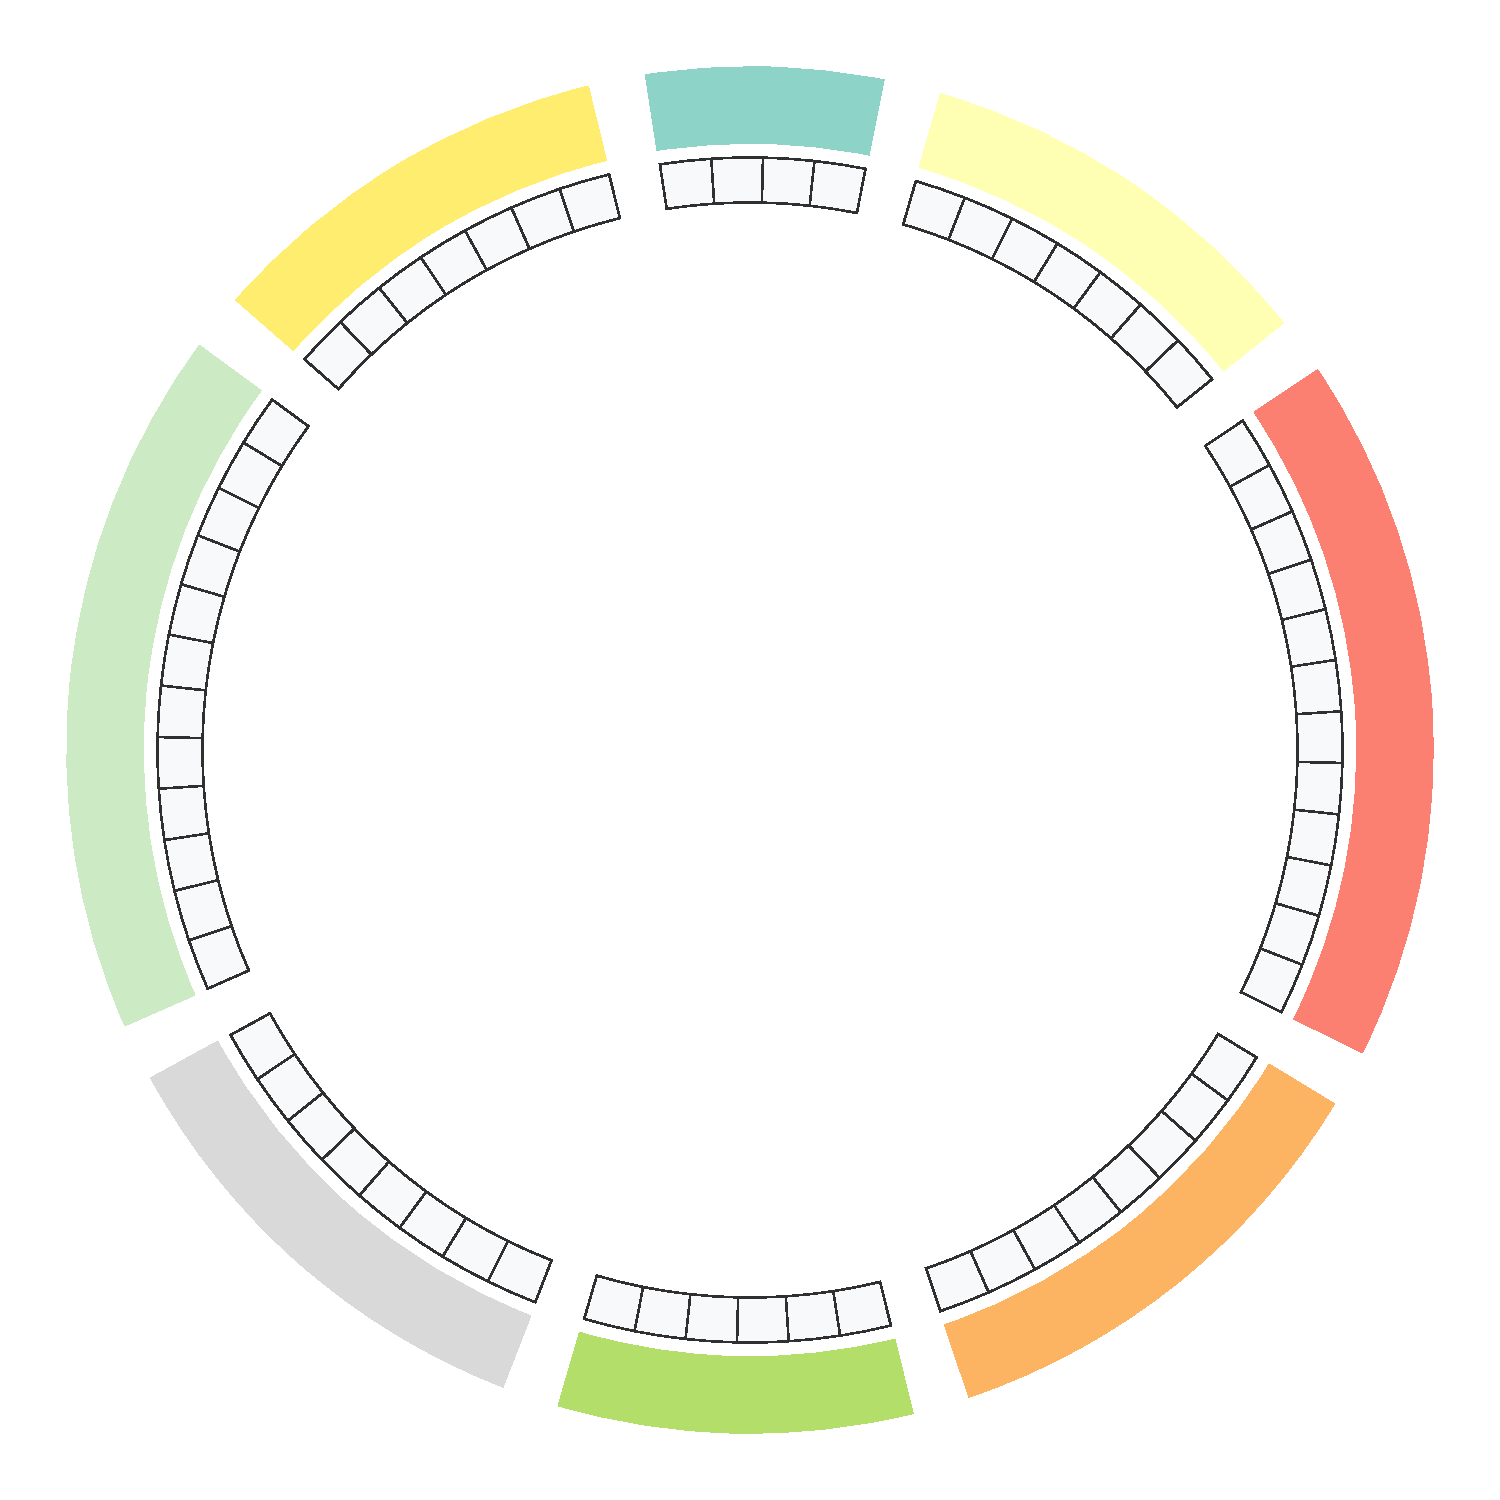
\includegraphics[width=\unitlength,page=1]{../Tesis_document/Figures/Objective_2/circonnecitvity_bad_2.pdf}}%
    \put(0.46180677,0.92326247){\color[rgb]{0,0,0}\rotatebox{-1.25000007}{\makebox(0,0)[lt]{\lineheight{1.25}\smash{\begin{tabular}[t]{l} \LARGE Frontal\end{tabular}}}}}%
    \put(0.6611217,0.90027212){\color[rgb]{0,0,0}\rotatebox{-33.7500015}{\makebox(0,0)[lt]{\lineheight{1.25}\smash{\begin{tabular}[t]{l} \LARGE Frontal Right\end{tabular}}}}}%
    \put(0.91543539,0.61899458){\color[rgb]{0,0,0}\rotatebox{-86.25000021}{\makebox(0,0)[lt]{\lineheight{1.25}\smash{\begin{tabular}[t]{l} \LARGE Central Right\end{tabular}}}}}%
    \put(0.69412404,0.09460069){\color[rgb]{0,0,0}\rotatebox{38.75000159}{\makebox(0,0)[lt]{\lineheight{1.25}\smash{\begin{tabular}[t]{l} \LARGE Posterior Right\end{tabular}}}}}%
    \put(0.42910616,0.06377129){\color[rgb]{0,0,0}\rotatebox{-1.25000007}{\makebox(0,0)[lt]{\lineheight{1.25}\smash{\begin{tabular}[t]{l} \LARGE Posterior\end{tabular}}}}}%
    \put(0.14234135,0.23152431){\color[rgb]{0,0,0}\rotatebox{-41.25000161}{\makebox(0,0)[lt]{\lineheight{1.25}\smash{\begin{tabular}[t]{l} \LARGE Posterior Left\end{tabular}}}}}%
    \put(0.07135272,0.46536153){\color[rgb]{0,0,0}\rotatebox{83.75000035}{\makebox(0,0)[lt]{\lineheight{1.25}\smash{\begin{tabular}[t]{l} \LARGE Central Left\end{tabular}}}}}%
    \put(0.21427494,0.82062025){\color[rgb]{0,0,0}\rotatebox{31.25000144}{\makebox(0,0)[lt]{\lineheight{1.25}\smash{\begin{tabular}[t]{l} \LARGE Frontal Left\end{tabular}}}}}%
    \put(0.43605391,0.86252168){\color[rgb]{0,0,0}\rotatebox{6.25000035}{\makebox(0,0)[lt]{\lineheight{1.25}\smash{\begin{tabular}[t]{l} \LARGE Fpz\end{tabular}}}}}%
    \put(0.46720967,0.86670052){\color[rgb]{0,0,0}\rotatebox{1.25000007}{\makebox(0,0)[lt]{\lineheight{1.25}\smash{\begin{tabular}[t]{l} \LARGE AFz\end{tabular}}}}}%
    \put(0.50877935,0.86754131){\color[rgb]{0,0,0}\rotatebox{-3.75000021}{\makebox(0,0)[lt]{\lineheight{1.25}\smash{\begin{tabular}[t]{l} \LARGE Fz\end{tabular}}}}}%
    \put(0.53119166,0.8668532){\color[rgb]{0,0,0}\rotatebox{-8.75000049}{\makebox(0,0)[lt]{\lineheight{1.25}\smash{\begin{tabular}[t]{l} \LARGE FCz\end{tabular}}}}}%
    \put(0.5937944,0.85607624){\color[rgb]{0,0,0}\rotatebox{-18.75000099}{\makebox(0,0)[lt]{\lineheight{1.25}\smash{\begin{tabular}[t]{l} \LARGE Fp2\end{tabular}}}}}%
    \put(0.62384588,0.8468219){\color[rgb]{0,0,0}\rotatebox{-23.7500012}{\makebox(0,0)[lt]{\lineheight{1.25}\smash{\begin{tabular}[t]{l} \LARGE AF4\end{tabular}}}}}%
    \put(0.65360212,0.83470824){\color[rgb]{0,0,0}\rotatebox{-28.75000137}{\makebox(0,0)[lt]{\lineheight{1.25}\smash{\begin{tabular}[t]{l} \LARGE AF8\end{tabular}}}}}%
    \put(0.69009266,0.81476648){\color[rgb]{0,0,0}\rotatebox{-33.7500015}{\makebox(0,0)[lt]{\lineheight{1.25}\smash{\begin{tabular}[t]{l} \LARGE F2\end{tabular}}}}}%
    \put(0.71680299,0.797001){\color[rgb]{0,0,0}\rotatebox{-38.75000159}{\makebox(0,0)[lt]{\lineheight{1.25}\smash{\begin{tabular}[t]{l} \LARGE F4\end{tabular}}}}}%
    \put(0.74186333,0.77697519){\color[rgb]{0,0,0}\rotatebox{-43.75000162}{\makebox(0,0)[lt]{\lineheight{1.25}\smash{\begin{tabular}[t]{l} \LARGE F6\end{tabular}}}}}%
    \put(0.76508295,0.75484144){\color[rgb]{0,0,0}\rotatebox{-48.75000161}{\makebox(0,0)[lt]{\lineheight{1.25}\smash{\begin{tabular}[t]{l} \LARGE F8\end{tabular}}}}}%
    \put(0.80027612,0.71323173){\color[rgb]{0,0,0}\rotatebox{-58.75000144}{\makebox(0,0)[lt]{\lineheight{1.25}\smash{\begin{tabular}[t]{l} \LARGE FC2\end{tabular}}}}}%
    \put(0.81771784,0.68624954){\color[rgb]{0,0,0}\rotatebox{-63.75000129}{\makebox(0,0)[lt]{\lineheight{1.25}\smash{\begin{tabular}[t]{l} \LARGE FC4\end{tabular}}}}}%
    \put(0.83274155,0.65784986){\color[rgb]{0,0,0}\rotatebox{-68.7500011}{\makebox(0,0)[lt]{\lineheight{1.25}\smash{\begin{tabular}[t]{l} \LARGE FC6\end{tabular}}}}}%
    \put(0.84564583,0.62683211){\color[rgb]{0,0,0}\rotatebox{-73.75000087}{\makebox(0,0)[lt]{\lineheight{1.25}\smash{\begin{tabular}[t]{l} \LARGE FT8\end{tabular}}}}}%
    \put(0.8566548,0.58983914){\color[rgb]{0,0,0}\rotatebox{-78.75000062}{\makebox(0,0)[lt]{\lineheight{1.25}\smash{\begin{tabular}[t]{l} \LARGE C2\end{tabular}}}}}%
    \put(0.86312762,0.55841274){\color[rgb]{0,0,0}\rotatebox{-83.75000035}{\makebox(0,0)[lt]{\lineheight{1.25}\smash{\begin{tabular}[t]{l} \LARGE C4\end{tabular}}}}}%
    \put(0.86683682,0.52654181){\color[rgb]{0,0,0}\rotatebox{-88.75000007}{\makebox(0,0)[lt]{\lineheight{1.25}\smash{\begin{tabular}[t]{l} \LARGE C6\end{tabular}}}}}%
    \put(0.86767468,0.4932562){\color[rgb]{0,0,0}\rotatebox{-93.74999979}{\makebox(0,0)[lt]{\lineheight{1.25}\smash{\begin{tabular}[t]{l} \LARGE T8\end{tabular}}}}}%
    \put(0.86714698,0.47071728){\color[rgb]{0,0,0}\rotatebox{-98.74999951}{\makebox(0,0)[lt]{\lineheight{1.25}\smash{\begin{tabular}[t]{l} \LARGE CP2\end{tabular}}}}}%
    \put(0.86319771,0.43882973){\color[rgb]{0,0,0}\rotatebox{-103.74999925}{\makebox(0,0)[lt]{\lineheight{1.25}\smash{\begin{tabular}[t]{l} \LARGE CP4\end{tabular}}}}}%
    \put(0.8564843,0.40740774){\color[rgb]{0,0,0}\rotatebox{-108.74999901}{\makebox(0,0)[lt]{\lineheight{1.25}\smash{\begin{tabular}[t]{l} \LARGE CP6\end{tabular}}}}}%
    \put(0.84656837,0.37557807){\color[rgb]{0,0,0}\rotatebox{-113.7499988}{\makebox(0,0)[lt]{\lineheight{1.25}\smash{\begin{tabular}[t]{l} \LARGE TP8\end{tabular}}}}}%
    \put(0.81498342,0.31023212){\color[rgb]{0,0,0}\rotatebox{-123.7499985}{\makebox(0,0)[lt]{\lineheight{1.25}\smash{\begin{tabular}[t]{l} \LARGE P2\end{tabular}}}}}%
    \put(0.79724546,0.28350163){\color[rgb]{0,0,0}\rotatebox{-128.74999841}{\makebox(0,0)[lt]{\lineheight{1.25}\smash{\begin{tabular}[t]{l} \LARGE P4\end{tabular}}}}}%
    \put(0.77724527,0.25841882){\color[rgb]{0,0,0}\rotatebox{-133.74999838}{\makebox(0,0)[lt]{\lineheight{1.25}\smash{\begin{tabular}[t]{l} \LARGE P6\end{tabular}}}}}%
    \put(0.75513508,0.23517458){\color[rgb]{0,0,0}\rotatebox{-138.74999839}{\makebox(0,0)[lt]{\lineheight{1.25}\smash{\begin{tabular}[t]{l} \LARGE P8\end{tabular}}}}}%
    \put(0.73820606,0.21916856){\color[rgb]{0,0,0}\rotatebox{-143.74999845}{\makebox(0,0)[lt]{\lineheight{1.25}\smash{\begin{tabular}[t]{l} \LARGE P10\end{tabular}}}}}%
    \put(0.71462317,0.20056822){\color[rgb]{0,0,0}\rotatebox{-148.74999856}{\makebox(0,0)[lt]{\lineheight{1.25}\smash{\begin{tabular}[t]{l} \LARGE PO4\end{tabular}}}}}%
    \put(0.68770925,0.183002){\color[rgb]{0,0,0}\rotatebox{-153.74999871}{\makebox(0,0)[lt]{\lineheight{1.25}\smash{\begin{tabular}[t]{l} \LARGE PO8\end{tabular}}}}}%
    \put(0.65155959,0.16481228){\color[rgb]{0,0,0}\rotatebox{-158.7499989}{\makebox(0,0)[lt]{\lineheight{1.25}\smash{\begin{tabular}[t]{l} \LARGE O2\end{tabular}}}}}%
    \put(0.59654369,0.14467879){\color[rgb]{0,0,0}\rotatebox{-168.74999938}{\makebox(0,0)[lt]{\lineheight{1.25}\smash{\begin{tabular}[t]{l} \LARGE CPz\end{tabular}}}}}%
    \put(0.55556517,0.13656049){\color[rgb]{0,0,0}\rotatebox{-173.74999965}{\makebox(0,0)[lt]{\lineheight{1.25}\smash{\begin{tabular}[t]{l} \LARGE Pz\end{tabular}}}}}%
    \put(0.52500134,0.13312954){\color[rgb]{0,0,0}\rotatebox{-178.74999993}{\makebox(0,0)[lt]{\lineheight{1.25}\smash{\begin{tabular}[t]{l} \LARGE Cz\end{tabular}}}}}%
    \put(0.50252448,0.13171781){\color[rgb]{0,0,0}\rotatebox{176.24999979}{\makebox(0,0)[lt]{\lineheight{1.25}\smash{\begin{tabular}[t]{l} \LARGE POz\end{tabular}}}}}%
    \put(0.46213774,0.13417351){\color[rgb]{0,0,0}\rotatebox{171.24999951}{\makebox(0,0)[lt]{\lineheight{1.25}\smash{\begin{tabular}[t]{l} \LARGE Oz\end{tabular}}}}}%
    \put(0.4237579,0.14049031){\color[rgb]{0,0,0}\rotatebox{166.24999925}{\makebox(0,0)[lt]{\lineheight{1.25}\smash{\begin{tabular}[t]{l} \LARGE Iz\end{tabular}}}}}%
    \put(0.3678114,0.15684901){\color[rgb]{0,0,0}\rotatebox{156.2499988}{\makebox(0,0)[lt]{\lineheight{1.25}\smash{\begin{tabular}[t]{l} \LARGE P1\end{tabular}}}}}%
    \put(0.33840684,0.1696758){\color[rgb]{0,0,0}\rotatebox{151.24999863}{\makebox(0,0)[lt]{\lineheight{1.25}\smash{\begin{tabular}[t]{l} \LARGE P3\end{tabular}}}}}%
    \put(0.3102321,0.18501654){\color[rgb]{0,0,0}\rotatebox{146.2499985}{\makebox(0,0)[lt]{\lineheight{1.25}\smash{\begin{tabular}[t]{l} \LARGE P5\end{tabular}}}}}%
    \put(0.28350161,0.20275451){\color[rgb]{0,0,0}\rotatebox{141.24999841}{\makebox(0,0)[lt]{\lineheight{1.25}\smash{\begin{tabular}[t]{l} \LARGE P7\end{tabular}}}}}%
    \put(0.2584188,0.22275471){\color[rgb]{0,0,0}\rotatebox{136.24999838}{\makebox(0,0)[lt]{\lineheight{1.25}\smash{\begin{tabular}[t]{l} \LARGE P9\end{tabular}}}}}%
    \put(0.24238617,0.23664165){\color[rgb]{0,0,0}\rotatebox{131.24999839}{\makebox(0,0)[lt]{\lineheight{1.25}\smash{\begin{tabular}[t]{l} \LARGE PO3\end{tabular}}}}}%
    \put(0.22041328,0.26009634){\color[rgb]{0,0,0}\rotatebox{126.24999845}{\makebox(0,0)[lt]{\lineheight{1.25}\smash{\begin{tabular}[t]{l} \LARGE PO7\end{tabular}}}}}%
    \put(0.19622258,0.2925382){\color[rgb]{0,0,0}\rotatebox{121.24999856}{\makebox(0,0)[lt]{\lineheight{1.25}\smash{\begin{tabular}[t]{l} \LARGE O1\end{tabular}}}}}%
    \put(0.16725842,0.34215016){\color[rgb]{0,0,0}\rotatebox{111.2499989}{\makebox(0,0)[lt]{\lineheight{1.25}\smash{\begin{tabular}[t]{l} \LARGE FC1\end{tabular}}}}}%
    \put(0.15476708,0.37175116){\color[rgb]{0,0,0}\rotatebox{106.24999913}{\makebox(0,0)[lt]{\lineheight{1.25}\smash{\begin{tabular}[t]{l} \LARGE FC3\end{tabular}}}}}%
    \put(0.14490317,0.40232821){\color[rgb]{0,0,0}\rotatebox{101.24999938}{\makebox(0,0)[lt]{\lineheight{1.25}\smash{\begin{tabular}[t]{l} \LARGE FC5\end{tabular}}}}}%
    \put(0.13758111,0.43511554){\color[rgb]{0,0,0}\rotatebox{96.24999965}{\makebox(0,0)[lt]{\lineheight{1.25}\smash{\begin{tabular}[t]{l} \LARGE FT7\end{tabular}}}}}%
    \put(0.13316315,0.4734582){\color[rgb]{0,0,0}\rotatebox{91.24999993}{\makebox(0,0)[lt]{\lineheight{1.25}\smash{\begin{tabular}[t]{l} \LARGE C1\end{tabular}}}}}%
    \put(0.1322458,0.50553113){\color[rgb]{0,0,0}\rotatebox{86.25000021}{\makebox(0,0)[lt]{\lineheight{1.25}\smash{\begin{tabular}[t]{l} \LARGE C3\end{tabular}}}}}%
    \put(0.13412729,0.53756199){\color[rgb]{0,0,0}\rotatebox{81.25000049}{\makebox(0,0)[lt]{\lineheight{1.25}\smash{\begin{tabular}[t]{l} \LARGE C5\end{tabular}}}}}%
    \put(0.13908213,0.5704874){\color[rgb]{0,0,0}\rotatebox{76.25000075}{\makebox(0,0)[lt]{\lineheight{1.25}\smash{\begin{tabular}[t]{l} \LARGE T7\end{tabular}}}}}%
    \put(0.14351567,0.59259229){\color[rgb]{0,0,0}\rotatebox{71.25000099}{\makebox(0,0)[lt]{\lineheight{1.25}\smash{\begin{tabular}[t]{l} \LARGE CP1\end{tabular}}}}}%
    \put(0.15294214,0.62330959){\color[rgb]{0,0,0}\rotatebox{66.2500012}{\makebox(0,0)[lt]{\lineheight{1.25}\smash{\begin{tabular}[t]{l} \LARGE CP3\end{tabular}}}}}%
    \put(0.16500994,0.65308845){\color[rgb]{0,0,0}\rotatebox{61.25000137}{\makebox(0,0)[lt]{\lineheight{1.25}\smash{\begin{tabular}[t]{l} \LARGE CP5\end{tabular}}}}}%
    \put(0.18030239,0.68271268){\color[rgb]{0,0,0}\rotatebox{56.2500015}{\makebox(0,0)[lt]{\lineheight{1.25}\smash{\begin{tabular}[t]{l} \LARGE TP7\end{tabular}}}}}%
    \put(0.21692455,0.73549096){\color[rgb]{0,0,0}\rotatebox{46.25000162}{\makebox(0,0)[lt]{\lineheight{1.25}\smash{\begin{tabular}[t]{l} \LARGE Fp1\end{tabular}}}}}%
    \put(0.23801217,0.75881577){\color[rgb]{0,0,0}\rotatebox{41.25000161}{\makebox(0,0)[lt]{\lineheight{1.25}\smash{\begin{tabular}[t]{l} \LARGE AF3\end{tabular}}}}}%
    \put(0.26156639,0.78066464){\color[rgb]{0,0,0}\rotatebox{36.25000155}{\makebox(0,0)[lt]{\lineheight{1.25}\smash{\begin{tabular}[t]{l} \LARGE AF7\end{tabular}}}}}%
    \put(0.29506135,0.80530853){\color[rgb]{0,0,0}\rotatebox{31.25000144}{\makebox(0,0)[lt]{\lineheight{1.25}\smash{\begin{tabular}[t]{l} \LARGE F1\end{tabular}}}}}%
    \put(0.32245059,0.82200834){\color[rgb]{0,0,0}\rotatebox{26.25000129}{\makebox(0,0)[lt]{\lineheight{1.25}\smash{\begin{tabular}[t]{l} \LARGE F3\end{tabular}}}}}%
    \put(0.35119109,0.83625745){\color[rgb]{0,0,0}\rotatebox{21.2500011}{\makebox(0,0)[lt]{\lineheight{1.25}\smash{\begin{tabular}[t]{l} \LARGE F5\end{tabular}}}}}%
    \put(0.38106412,0.84794741){\color[rgb]{0,0,0}\rotatebox{16.25000087}{\makebox(0,0)[lt]{\lineheight{1.25}\smash{\begin{tabular}[t]{l} \LARGE F7\end{tabular}}}}}%
  \end{picture}%
\endgroup%
}	
    \end{subfigure}
    \\
    \begin{subfigure}[b]{.3\linewidth}
        \centering
        \resizebox{1\linewidth}{!}{%% Creator: Inkscape 1.2.2 (b0a8486541, 2022-12-01), www.inkscape.org
%% PDF/EPS/PS + LaTeX output extension by Johan Engelen, 2010
%% Accompanies image file 'topoplot_good_2.pdf' (pdf, eps, ps)
%%
%% To include the image in your LaTeX document, write
%%   \input{<filename>.pdf_tex}
%%  instead of
%%   \includegraphics{<filename>.pdf}
%% To scale the image, write
%%   \def\svgwidth{<desired width>}
%%   \input{<filename>.pdf_tex}
%%  instead of
%%   \includegraphics[width=<desired width>]{<filename>.pdf}
%%
%% Images with a different path to the parent latex file can
%% be accessed with the `import' package (which may need to be
%% installed) using
%%   \usepackage{import}
%% in the preamble, and then including the image with
%%   \import{<path to file>}{<filename>.pdf_tex}
%% Alternatively, one can specify
%%   \graphicspath{{<path to file>/}}
%% 
%% For more information, please see info/svg-inkscape on CTAN:
%%   http://tug.ctan.org/tex-archive/info/svg-inkscape
%%
\begingroup%
  \makeatletter%
  \providecommand\color[2][]{%
    \errmessage{(Inkscape) Color is used for the text in Inkscape, but the package 'color.sty' is not loaded}%
    \renewcommand\color[2][]{}%
  }%
  \providecommand\transparent[1]{%
    \errmessage{(Inkscape) Transparency is used (non-zero) for the text in Inkscape, but the package 'transparent.sty' is not loaded}%
    \renewcommand\transparent[1]{}%
  }%
  \providecommand\rotatebox[2]{#2}%
  \newcommand*\fsize{\dimexpr\f@size pt\relax}%
  \newcommand*\lineheight[1]{\fontsize{\fsize}{#1\fsize}\selectfont}%
  \ifx\svgwidth\undefined%
    \setlength{\unitlength}{555.09296567bp}%
    \ifx\svgscale\undefined%
      \relax%
    \else%
      \setlength{\unitlength}{\unitlength * \real{\svgscale}}%
    \fi%
  \else%
    \setlength{\unitlength}{\svgwidth}%
  \fi%
  \global\let\svgwidth\undefined%
  \global\let\svgscale\undefined%
  \makeatother%
  \begin{picture}(1,1.02003514)%
    \lineheight{1}%
    \setlength\tabcolsep{0pt}%
    \put(0,0){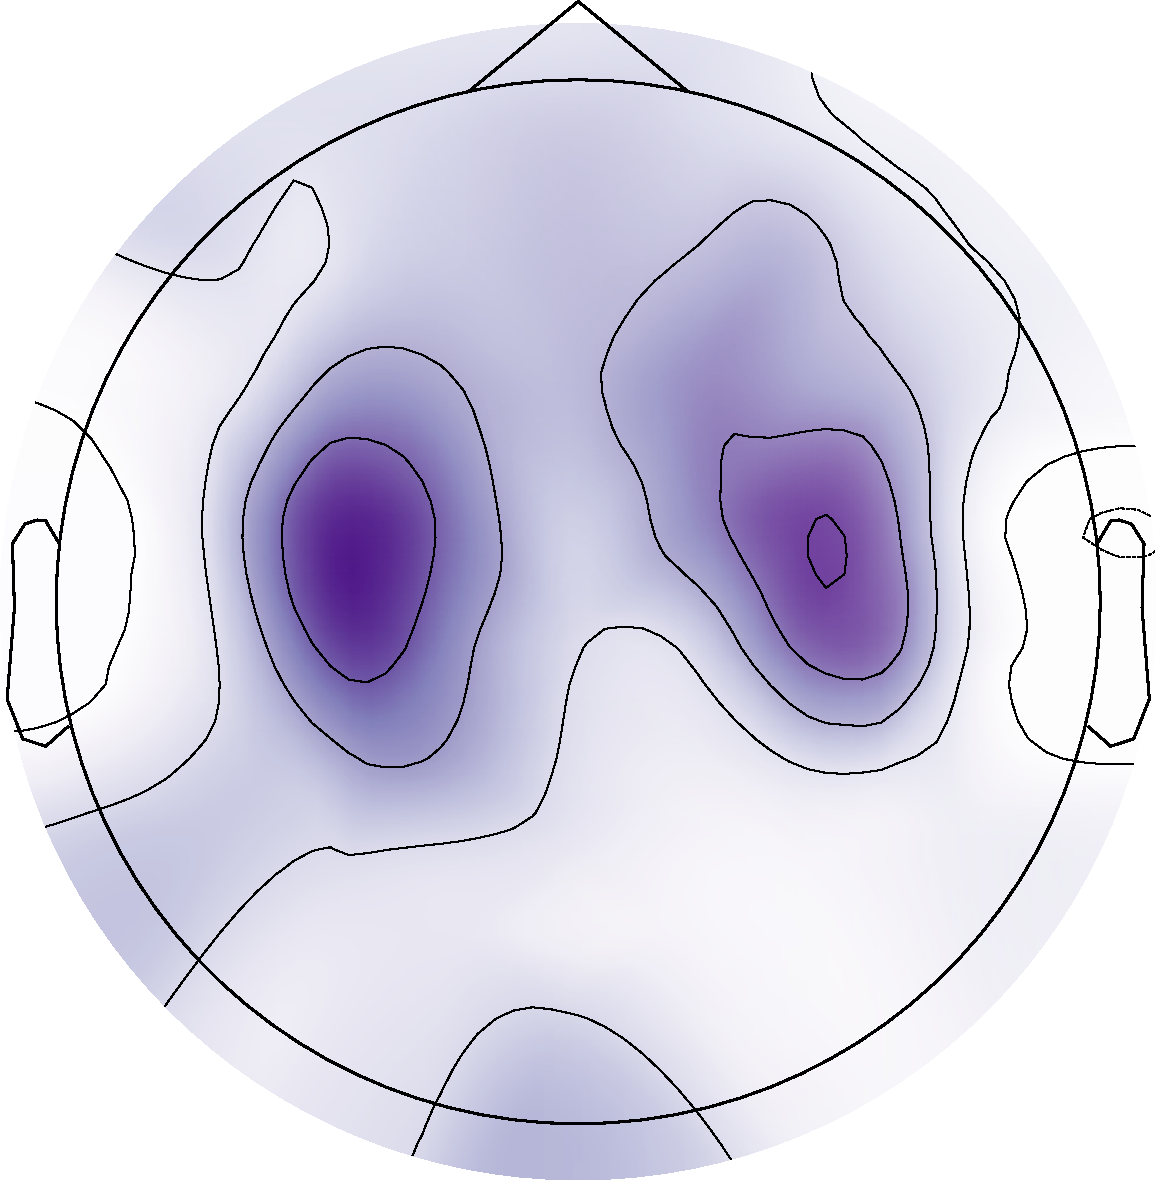
\includegraphics[width=\unitlength,page=1]{Figures/Objective_2/topoplot_good_2.pdf}}%
    \put(0.35967033,0.97370124){\color[rgb]{0,0,0}\makebox(0,0)[lt]{\lineheight{1.25}\smash{\begin{tabular}[t]{l} \Large Fp1\end{tabular}}}}%
    \put(0.48360262,0.98294946){\color[rgb]{0,0,0}\makebox(0,0)[lt]{\lineheight{1.25}\smash{\begin{tabular}[t]{l} \Large Fpz\end{tabular}}}}%
    \put(0.6067521,0.97720871){\color[rgb]{0,0,0}\makebox(0,0)[lt]{\lineheight{1.25}\smash{\begin{tabular}[t]{l} \Large Fp2\end{tabular}}}}%
    \put(0.25167325,0.91234291){\color[rgb]{0,0,0}\makebox(0,0)[lt]{\lineheight{1.25}\smash{\begin{tabular}[t]{l} \Large AF7\end{tabular}}}}%
    \put(0.35594832,0.90619769){\color[rgb]{0,0,0}\makebox(0,0)[lt]{\lineheight{1.25}\smash{\begin{tabular}[t]{l} \Large AF3\end{tabular}}}}%
    \put(0.48426543,0.90789205){\color[rgb]{0,0,0}\makebox(0,0)[lt]{\lineheight{1.25}\smash{\begin{tabular}[t]{l} \Large AFz\end{tabular}}}}%
    \put(0.61635461,0.90817399){\color[rgb]{0,0,0}\makebox(0,0)[lt]{\lineheight{1.25}\smash{\begin{tabular}[t]{l} \Large AF4\end{tabular}}}}%
    \put(0.71557361,0.9154296){\color[rgb]{0,0,0}\makebox(0,0)[lt]{\lineheight{1.25}\smash{\begin{tabular}[t]{l} \Large AF8\end{tabular}}}}%
    \put(0.19542927,0.798521){\color[rgb]{0,0,0}\makebox(0,0)[lt]{\lineheight{1.25}\smash{\begin{tabular}[t]{l} \Large F7\end{tabular}}}}%
    \put(0.24637794,0.79533024){\color[rgb]{0,0,0}\makebox(0,0)[lt]{\lineheight{1.25}\smash{\begin{tabular}[t]{l} \Large F5\end{tabular}}}}%
    \put(0.31178457,0.79866269){\color[rgb]{0,0,0}\makebox(0,0)[lt]{\lineheight{1.25}\smash{\begin{tabular}[t]{l} \Large F3\end{tabular}}}}%
    \put(0.39486162,0.80350283){\color[rgb]{0,0,0}\makebox(0,0)[lt]{\lineheight{1.25}\smash{\begin{tabular}[t]{l} \Large F1\end{tabular}}}}%
    \put(0.48898287,0.80600162){\color[rgb]{0,0,0}\makebox(0,0)[lt]{\lineheight{1.25}\smash{\begin{tabular}[t]{l} \Large Fz\end{tabular}}}}%
    \put(0.58636468,0.80532111){\color[rgb]{0,0,0}\makebox(0,0)[lt]{\lineheight{1.25}\smash{\begin{tabular}[t]{l} \Large F2\end{tabular}}}}%
    \put(0.66805384,0.80209938){\color[rgb]{0,0,0}\makebox(0,0)[lt]{\lineheight{1.25}\smash{\begin{tabular}[t]{l} \Large F4\end{tabular}}}}%
    \put(0.7403106,0.80128699){\color[rgb]{0,0,0}\makebox(0,0)[lt]{\lineheight{1.25}\smash{\begin{tabular}[t]{l} \Large F6\end{tabular}}}}%
    \put(0.78864346,0.80554228){\color[rgb]{0,0,0}\makebox(0,0)[lt]{\lineheight{1.25}\smash{\begin{tabular}[t]{l} \Large F8\end{tabular}}}}%
    \put(0.15454617,0.6781539){\color[rgb]{0,0,0}\makebox(0,0)[lt]{\lineheight{1.25}\smash{\begin{tabular}[t]{l} \Large FT7\end{tabular}}}}%
    \put(0.20615052,0.6799757){\color[rgb]{0,0,0}\makebox(0,0)[lt]{\lineheight{1.25}\smash{\begin{tabular}[t]{l} \Large FC5\end{tabular}}}}%
    \put(0.28304226,0.6858006){\color[rgb]{0,0,0}\makebox(0,0)[lt]{\lineheight{1.25}\smash{\begin{tabular}[t]{l} \Large FC3\end{tabular}}}}%
    \put(0.37439804,0.69273688){\color[rgb]{0,0,0}\makebox(0,0)[lt]{\lineheight{1.25}\smash{\begin{tabular}[t]{l} \Large FC1\end{tabular}}}}%
    \put(0.48466801,0.69558686){\color[rgb]{0,0,0}\makebox(0,0)[lt]{\lineheight{1.25}\smash{\begin{tabular}[t]{l} \Large FCz\end{tabular}}}}%
    \put(0.59323604,0.6930023){\color[rgb]{0,0,0}\makebox(0,0)[lt]{\lineheight{1.25}\smash{\begin{tabular}[t]{l} \Large FC2\end{tabular}}}}%
    \put(0.68863996,0.68755182){\color[rgb]{0,0,0}\makebox(0,0)[lt]{\lineheight{1.25}\smash{\begin{tabular}[t]{l} \Large FC4\end{tabular}}}}%
    \put(0.76580891,0.68247925){\color[rgb]{0,0,0}\makebox(0,0)[lt]{\lineheight{1.25}\smash{\begin{tabular}[t]{l} \Large FC6\end{tabular}}}}%
    \put(0.81263958,0.68079027){\color[rgb]{0,0,0}\makebox(0,0)[lt]{\lineheight{1.25}\smash{\begin{tabular}[t]{l} \Large FT8\end{tabular}}}}%
    \put(0.15304432,0.55517344){\color[rgb]{0,0,0}\makebox(0,0)[lt]{\lineheight{1.25}\smash{\begin{tabular}[t]{l} \Large T7\end{tabular}}}}%
    \put(0.20793195,0.56319456){\color[rgb]{0,0,0}\makebox(0,0)[lt]{\lineheight{1.25}\smash{\begin{tabular}[t]{l} \Large C5\end{tabular}}}}%
    \put(0.2758494,0.57156896){\color[rgb]{0,0,0}\makebox(0,0)[lt]{\lineheight{1.25}\smash{\begin{tabular}[t]{l} \Large C3\end{tabular}}}}%
    \put(0.37455147,0.57777093){\color[rgb]{0,0,0}\makebox(0,0)[lt]{\lineheight{1.25}\smash{\begin{tabular}[t]{l} \Large C1\end{tabular}}}}%
    \put(0.48810416,0.58059853){\color[rgb]{0,0,0}\makebox(0,0)[lt]{\lineheight{1.25}\smash{\begin{tabular}[t]{l} \Large Cz\end{tabular}}}}%
    \put(0.60220533,0.57776){\color[rgb]{0,0,0}\makebox(0,0)[lt]{\lineheight{1.25}\smash{\begin{tabular}[t]{l} \Large C2\end{tabular}}}}%
    \put(0.70116505,0.57214881){\color[rgb]{0,0,0}\makebox(0,0)[lt]{\lineheight{1.25}\smash{\begin{tabular}[t]{l} \Large C4\end{tabular}}}}%
    \put(0.77358016,0.56454473){\color[rgb]{0,0,0}\makebox(0,0)[lt]{\lineheight{1.25}\smash{\begin{tabular}[t]{l} \Large C6\end{tabular}}}}%
    \put(0.8193488,0.55648853){\color[rgb]{0,0,0}\makebox(0,0)[lt]{\lineheight{1.25}\smash{\begin{tabular}[t]{l} \Large T8\end{tabular}}}}%
    \put(0.15179752,0.43852856){\color[rgb]{0,0,0}\makebox(0,0)[lt]{\lineheight{1.25}\smash{\begin{tabular}[t]{l} \Large TP7\end{tabular}}}}%
    \put(0.20911876,0.45089997){\color[rgb]{0,0,0}\makebox(0,0)[lt]{\lineheight{1.25}\smash{\begin{tabular}[t]{l} \Large CP5\end{tabular}}}}%
    \put(0.27925236,0.45863292){\color[rgb]{0,0,0}\makebox(0,0)[lt]{\lineheight{1.25}\smash{\begin{tabular}[t]{l} \Large CP3\end{tabular}}}}%
    \put(0.37303238,0.46333522){\color[rgb]{0,0,0}\makebox(0,0)[lt]{\lineheight{1.25}\smash{\begin{tabular}[t]{l} \Large CP1\end{tabular}}}}%
    \put(0.48387009,0.46467519){\color[rgb]{0,0,0}\makebox(0,0)[lt]{\lineheight{1.25}\smash{\begin{tabular}[t]{l} \Large CPz\end{tabular}}}}%
    \put(0.59956053,0.46310679){\color[rgb]{0,0,0}\makebox(0,0)[lt]{\lineheight{1.25}\smash{\begin{tabular}[t]{l} \Large CP2\end{tabular}}}}%
    \put(0.69365975,0.45836576){\color[rgb]{0,0,0}\makebox(0,0)[lt]{\lineheight{1.25}\smash{\begin{tabular}[t]{l} \Large CP4\end{tabular}}}}%
    \put(0.76588976,0.45053107){\color[rgb]{0,0,0}\makebox(0,0)[lt]{\lineheight{1.25}\smash{\begin{tabular}[t]{l} \Large CP6\end{tabular}}}}%
    \put(0.81110016,0.43829595){\color[rgb]{0,0,0}\makebox(0,0)[lt]{\lineheight{1.25}\smash{\begin{tabular}[t]{l} \Large TP8\end{tabular}}}}%
    \put(0.14280782,0.28880787){\color[rgb]{0,0,0}\makebox(0,0)[lt]{\lineheight{1.25}\smash{\begin{tabular}[t]{l} \Large P9\end{tabular}}}}%
    \put(0.21177289,0.33788403){\color[rgb]{0,0,0}\makebox(0,0)[lt]{\lineheight{1.25}\smash{\begin{tabular}[t]{l} \Large P7\end{tabular}}}}%
    \put(0.25524807,0.34872807){\color[rgb]{0,0,0}\makebox(0,0)[lt]{\lineheight{1.25}\smash{\begin{tabular}[t]{l} \Large P5\end{tabular}}}}%
    \put(0.31471024,0.35396156){\color[rgb]{0,0,0}\makebox(0,0)[lt]{\lineheight{1.25}\smash{\begin{tabular}[t]{l} \Large P3\end{tabular}}}}%
    \put(0.39657717,0.35639095){\color[rgb]{0,0,0}\makebox(0,0)[lt]{\lineheight{1.25}\smash{\begin{tabular}[t]{l} \Large P1\end{tabular}}}}%
    \put(0.48761854,0.35703059){\color[rgb]{0,0,0}\makebox(0,0)[lt]{\lineheight{1.25}\smash{\begin{tabular}[t]{l} \Large Pz\end{tabular}}}}%
    \put(0.58532304,0.35619035){\color[rgb]{0,0,0}\makebox(0,0)[lt]{\lineheight{1.25}\smash{\begin{tabular}[t]{l} \Large P2\end{tabular}}}}%
    \put(0.66479963,0.35384721){\color[rgb]{0,0,0}\makebox(0,0)[lt]{\lineheight{1.25}\smash{\begin{tabular}[t]{l} \Large P4\end{tabular}}}}%
    \put(0.71635389,0.34901586){\color[rgb]{0,0,0}\makebox(0,0)[lt]{\lineheight{1.25}\smash{\begin{tabular}[t]{l} \Large P6\end{tabular}}}}%
    \put(0.75830593,0.33820066){\color[rgb]{0,0,0}\makebox(0,0)[lt]{\lineheight{1.25}\smash{\begin{tabular}[t]{l} \Large P8\end{tabular}}}}%
    \put(0.82302573,0.28323066){\color[rgb]{0,0,0}\makebox(0,0)[lt]{\lineheight{1.25}\smash{\begin{tabular}[t]{l} \Large P10\end{tabular}}}}%
    \put(0.27724405,0.2534568){\color[rgb]{0,0,0}\makebox(0,0)[lt]{\lineheight{1.25}\smash{\begin{tabular}[t]{l} \Large PO7\end{tabular}}}}%
    \put(0.35847067,0.27198302){\color[rgb]{0,0,0}\makebox(0,0)[lt]{\lineheight{1.25}\smash{\begin{tabular}[t]{l} \Large PO3\end{tabular}}}}%
    \put(0.48179538,0.27697404){\color[rgb]{0,0,0}\makebox(0,0)[lt]{\lineheight{1.25}\smash{\begin{tabular}[t]{l} \Large POz\end{tabular}}}}%
    \put(0.60260463,0.27132587){\color[rgb]{0,0,0}\makebox(0,0)[lt]{\lineheight{1.25}\smash{\begin{tabular}[t]{l} \Large PO4\end{tabular}}}}%
    \put(0.68406127,0.25242018){\color[rgb]{0,0,0}\makebox(0,0)[lt]{\lineheight{1.25}\smash{\begin{tabular}[t]{l} \Large PO8\end{tabular}}}}%
    \put(0.37725444,0.20621895){\color[rgb]{0,0,0}\makebox(0,0)[lt]{\lineheight{1.25}\smash{\begin{tabular}[t]{l} \Large O1\end{tabular}}}}%
    \put(0.4844748,0.20522486){\color[rgb]{0,0,0}\makebox(0,0)[lt]{\lineheight{1.25}\smash{\begin{tabular}[t]{l} \Large Oz\end{tabular}}}}%
    \put(0.59051739,0.20723665){\color[rgb]{0,0,0}\makebox(0,0)[lt]{\lineheight{1.25}\smash{\begin{tabular}[t]{l} \Large O2\end{tabular}}}}%
    \put(0.48585918,0.13245896){\color[rgb]{0,0,0}\makebox(0,0)[lt]{\lineheight{1.25}\smash{\begin{tabular}[t]{l} \Large Iz\end{tabular}}}}%
  \end{picture}%
\endgroup%
}	
    \end{subfigure}
    ~ 
    \begin{subfigure}[b]{.3\linewidth}
        \centering
        \resizebox{1\linewidth}{!}{%% Creator: Inkscape 1.2.2 (b0a8486541, 2022-12-01), www.inkscape.org
%% PDF/EPS/PS + LaTeX output extension by Johan Engelen, 2010
%% Accompanies image file 'topoplot_medium_2.pdf' (pdf, eps, ps)
%%
%% To include the image in your LaTeX document, write
%%   \input{<filename>.pdf_tex}
%%  instead of
%%   \includegraphics{<filename>.pdf}
%% To scale the image, write
%%   \def\svgwidth{<desired width>}
%%   \input{<filename>.pdf_tex}
%%  instead of
%%   \includegraphics[width=<desired width>]{<filename>.pdf}
%%
%% Images with a different path to the parent latex file can
%% be accessed with the `import' package (which may need to be
%% installed) using
%%   \usepackage{import}
%% in the preamble, and then including the image with
%%   \import{<path to file>}{<filename>.pdf_tex}
%% Alternatively, one can specify
%%   \graphicspath{{<path to file>/}}
%% 
%% For more information, please see info/svg-inkscape on CTAN:
%%   http://tug.ctan.org/tex-archive/info/svg-inkscape
%%
\begingroup%
  \makeatletter%
  \providecommand\color[2][]{%
    \errmessage{(Inkscape) Color is used for the text in Inkscape, but the package 'color.sty' is not loaded}%
    \renewcommand\color[2][]{}%
  }%
  \providecommand\transparent[1]{%
    \errmessage{(Inkscape) Transparency is used (non-zero) for the text in Inkscape, but the package 'transparent.sty' is not loaded}%
    \renewcommand\transparent[1]{}%
  }%
  \providecommand\rotatebox[2]{#2}%
  \newcommand*\fsize{\dimexpr\f@size pt\relax}%
  \newcommand*\lineheight[1]{\fontsize{\fsize}{#1\fsize}\selectfont}%
  \ifx\svgwidth\undefined%
    \setlength{\unitlength}{555.0933117bp}%
    \ifx\svgscale\undefined%
      \relax%
    \else%
      \setlength{\unitlength}{\unitlength * \real{\svgscale}}%
    \fi%
  \else%
    \setlength{\unitlength}{\svgwidth}%
  \fi%
  \global\let\svgwidth\undefined%
  \global\let\svgscale\undefined%
  \makeatother%
  \begin{picture}(1,1.0200345)%
    \lineheight{1}%
    \setlength\tabcolsep{0pt}%
    \put(0,0){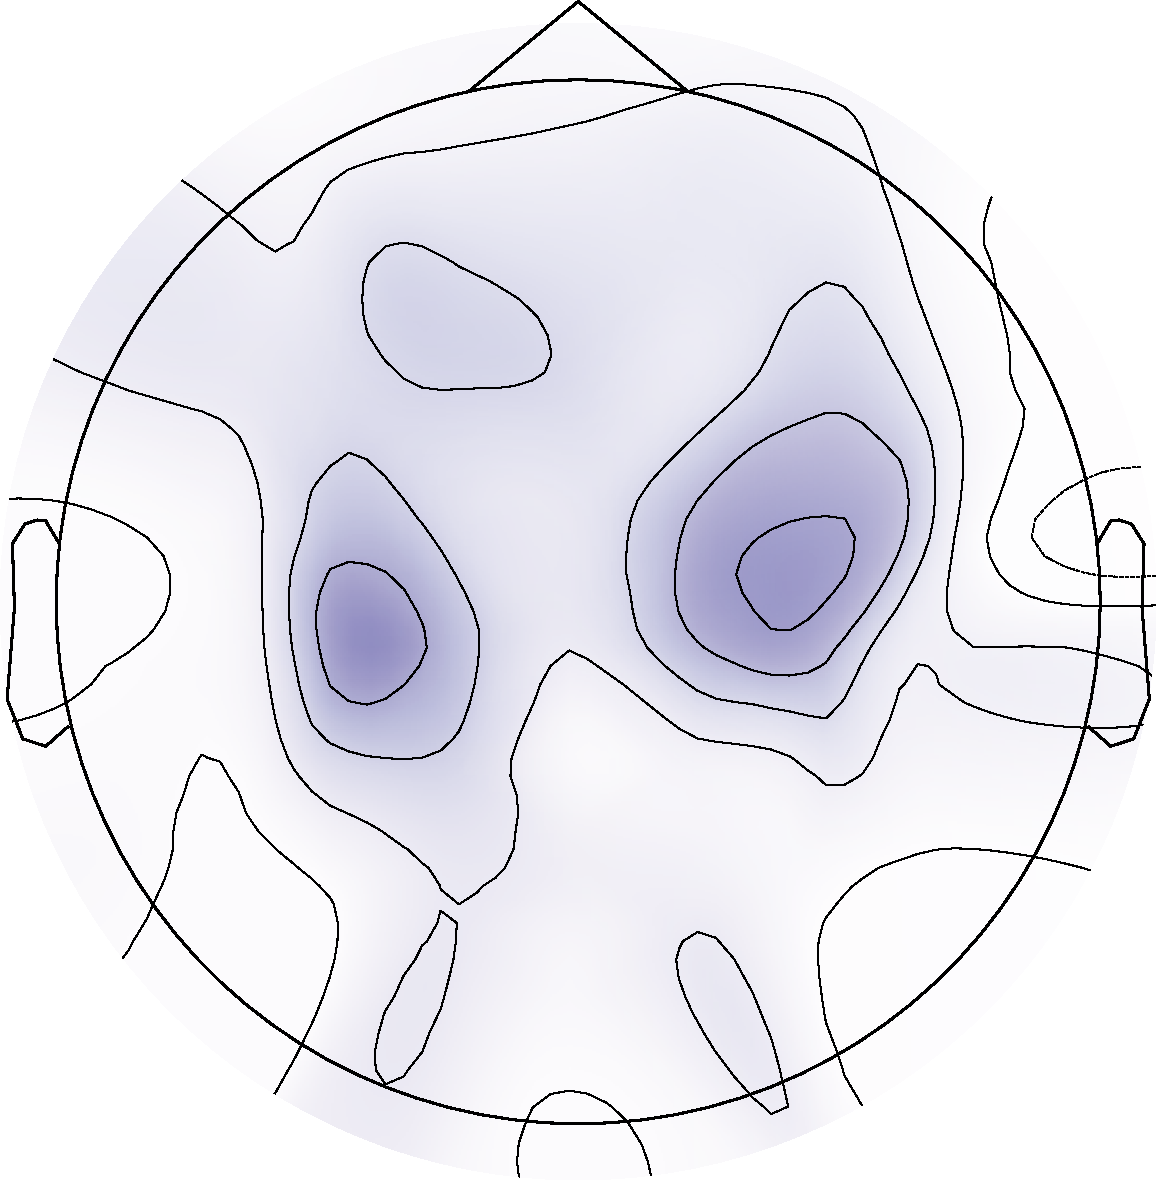
\includegraphics[width=\unitlength,page=1]{Figures/Objective_2/topoplot_medium_2.pdf}}%
    \put(0.35967013,0.97370064){\color[rgb]{0,0,0}\makebox(0,0)[lt]{\lineheight{1.25}\smash{\begin{tabular}[t]{l} \Large Fp1\end{tabular}}}}%
    \put(0.48360235,0.98294885){\color[rgb]{0,0,0}\makebox(0,0)[lt]{\lineheight{1.25}\smash{\begin{tabular}[t]{l} \Large Fpz\end{tabular}}}}%
    \put(0.60675175,0.9772081){\color[rgb]{0,0,0}\makebox(0,0)[lt]{\lineheight{1.25}\smash{\begin{tabular}[t]{l} \Large Fp2\end{tabular}}}}%
    \put(0.25167312,0.91234234){\color[rgb]{0,0,0}\makebox(0,0)[lt]{\lineheight{1.25}\smash{\begin{tabular}[t]{l} \Large AF7\end{tabular}}}}%
    \put(0.35594813,0.90619712){\color[rgb]{0,0,0}\makebox(0,0)[lt]{\lineheight{1.25}\smash{\begin{tabular}[t]{l} \Large AF3\end{tabular}}}}%
    \put(0.48426516,0.90789149){\color[rgb]{0,0,0}\makebox(0,0)[lt]{\lineheight{1.25}\smash{\begin{tabular}[t]{l} \Large AFz\end{tabular}}}}%
    \put(0.61635426,0.90817342){\color[rgb]{0,0,0}\makebox(0,0)[lt]{\lineheight{1.25}\smash{\begin{tabular}[t]{l} \Large AF4\end{tabular}}}}%
    \put(0.7155732,0.91542903){\color[rgb]{0,0,0}\makebox(0,0)[lt]{\lineheight{1.25}\smash{\begin{tabular}[t]{l} \Large AF8\end{tabular}}}}%
    \put(0.19542918,0.7985205){\color[rgb]{0,0,0}\makebox(0,0)[lt]{\lineheight{1.25}\smash{\begin{tabular}[t]{l} \Large F7\end{tabular}}}}%
    \put(0.24637782,0.79532974){\color[rgb]{0,0,0}\makebox(0,0)[lt]{\lineheight{1.25}\smash{\begin{tabular}[t]{l} \Large F5\end{tabular}}}}%
    \put(0.3117844,0.79866219){\color[rgb]{0,0,0}\makebox(0,0)[lt]{\lineheight{1.25}\smash{\begin{tabular}[t]{l} \Large F3\end{tabular}}}}%
    \put(0.3948614,0.80350233){\color[rgb]{0,0,0}\makebox(0,0)[lt]{\lineheight{1.25}\smash{\begin{tabular}[t]{l} \Large F1\end{tabular}}}}%
    \put(0.4889826,0.80600112){\color[rgb]{0,0,0}\makebox(0,0)[lt]{\lineheight{1.25}\smash{\begin{tabular}[t]{l} \Large Fz\end{tabular}}}}%
    \put(0.58636435,0.8053206){\color[rgb]{0,0,0}\makebox(0,0)[lt]{\lineheight{1.25}\smash{\begin{tabular}[t]{l} \Large F2\end{tabular}}}}%
    \put(0.66805346,0.80209888){\color[rgb]{0,0,0}\makebox(0,0)[lt]{\lineheight{1.25}\smash{\begin{tabular}[t]{l} \Large F4\end{tabular}}}}%
    \put(0.74031017,0.80128649){\color[rgb]{0,0,0}\makebox(0,0)[lt]{\lineheight{1.25}\smash{\begin{tabular}[t]{l} \Large F6\end{tabular}}}}%
    \put(0.788643,0.80554177){\color[rgb]{0,0,0}\makebox(0,0)[lt]{\lineheight{1.25}\smash{\begin{tabular}[t]{l} \Large F8\end{tabular}}}}%
    \put(0.15454611,0.67815348){\color[rgb]{0,0,0}\makebox(0,0)[lt]{\lineheight{1.25}\smash{\begin{tabular}[t]{l} \Large FT7\end{tabular}}}}%
    \put(0.20615042,0.67997528){\color[rgb]{0,0,0}\makebox(0,0)[lt]{\lineheight{1.25}\smash{\begin{tabular}[t]{l} \Large FC5\end{tabular}}}}%
    \put(0.28304212,0.68580018){\color[rgb]{0,0,0}\makebox(0,0)[lt]{\lineheight{1.25}\smash{\begin{tabular}[t]{l} \Large FC3\end{tabular}}}}%
    \put(0.37439784,0.69273645){\color[rgb]{0,0,0}\makebox(0,0)[lt]{\lineheight{1.25}\smash{\begin{tabular}[t]{l} \Large FC1\end{tabular}}}}%
    \put(0.48466774,0.69558642){\color[rgb]{0,0,0}\makebox(0,0)[lt]{\lineheight{1.25}\smash{\begin{tabular}[t]{l} \Large FCz\end{tabular}}}}%
    \put(0.5932357,0.69300187){\color[rgb]{0,0,0}\makebox(0,0)[lt]{\lineheight{1.25}\smash{\begin{tabular}[t]{l} \Large FC2\end{tabular}}}}%
    \put(0.68863956,0.68755139){\color[rgb]{0,0,0}\makebox(0,0)[lt]{\lineheight{1.25}\smash{\begin{tabular}[t]{l} \Large FC4\end{tabular}}}}%
    \put(0.76580846,0.68247882){\color[rgb]{0,0,0}\makebox(0,0)[lt]{\lineheight{1.25}\smash{\begin{tabular}[t]{l} \Large FC6\end{tabular}}}}%
    \put(0.81263911,0.68078985){\color[rgb]{0,0,0}\makebox(0,0)[lt]{\lineheight{1.25}\smash{\begin{tabular}[t]{l} \Large FT8\end{tabular}}}}%
    \put(0.15304425,0.55517309){\color[rgb]{0,0,0}\makebox(0,0)[lt]{\lineheight{1.25}\smash{\begin{tabular}[t]{l} \Large T7\end{tabular}}}}%
    \put(0.20793185,0.56319421){\color[rgb]{0,0,0}\makebox(0,0)[lt]{\lineheight{1.25}\smash{\begin{tabular}[t]{l} \Large C5\end{tabular}}}}%
    \put(0.27584926,0.57156861){\color[rgb]{0,0,0}\makebox(0,0)[lt]{\lineheight{1.25}\smash{\begin{tabular}[t]{l} \Large C3\end{tabular}}}}%
    \put(0.37455127,0.57777057){\color[rgb]{0,0,0}\makebox(0,0)[lt]{\lineheight{1.25}\smash{\begin{tabular}[t]{l} \Large C1\end{tabular}}}}%
    \put(0.48810388,0.58059817){\color[rgb]{0,0,0}\makebox(0,0)[lt]{\lineheight{1.25}\smash{\begin{tabular}[t]{l} \Large Cz\end{tabular}}}}%
    \put(0.60220498,0.57775964){\color[rgb]{0,0,0}\makebox(0,0)[lt]{\lineheight{1.25}\smash{\begin{tabular}[t]{l} \Large C2\end{tabular}}}}%
    \put(0.70116465,0.57214845){\color[rgb]{0,0,0}\makebox(0,0)[lt]{\lineheight{1.25}\smash{\begin{tabular}[t]{l} \Large C4\end{tabular}}}}%
    \put(0.77357971,0.56454438){\color[rgb]{0,0,0}\makebox(0,0)[lt]{\lineheight{1.25}\smash{\begin{tabular}[t]{l} \Large C6\end{tabular}}}}%
    \put(0.81934832,0.55648819){\color[rgb]{0,0,0}\makebox(0,0)[lt]{\lineheight{1.25}\smash{\begin{tabular}[t]{l} \Large T8\end{tabular}}}}%
    \put(0.15179745,0.43852829){\color[rgb]{0,0,0}\makebox(0,0)[lt]{\lineheight{1.25}\smash{\begin{tabular}[t]{l} \Large TP7\end{tabular}}}}%
    \put(0.20911866,0.45089969){\color[rgb]{0,0,0}\makebox(0,0)[lt]{\lineheight{1.25}\smash{\begin{tabular}[t]{l} \Large CP5\end{tabular}}}}%
    \put(0.27925222,0.45863264){\color[rgb]{0,0,0}\makebox(0,0)[lt]{\lineheight{1.25}\smash{\begin{tabular}[t]{l} \Large CP3\end{tabular}}}}%
    \put(0.37303217,0.46333493){\color[rgb]{0,0,0}\makebox(0,0)[lt]{\lineheight{1.25}\smash{\begin{tabular}[t]{l} \Large CP1\end{tabular}}}}%
    \put(0.48386982,0.4646749){\color[rgb]{0,0,0}\makebox(0,0)[lt]{\lineheight{1.25}\smash{\begin{tabular}[t]{l} \Large CPz\end{tabular}}}}%
    \put(0.59956018,0.4631065){\color[rgb]{0,0,0}\makebox(0,0)[lt]{\lineheight{1.25}\smash{\begin{tabular}[t]{l} \Large CP2\end{tabular}}}}%
    \put(0.69365935,0.45836548){\color[rgb]{0,0,0}\makebox(0,0)[lt]{\lineheight{1.25}\smash{\begin{tabular}[t]{l} \Large CP4\end{tabular}}}}%
    \put(0.76588931,0.45053079){\color[rgb]{0,0,0}\makebox(0,0)[lt]{\lineheight{1.25}\smash{\begin{tabular}[t]{l} \Large CP6\end{tabular}}}}%
    \put(0.81109969,0.43829568){\color[rgb]{0,0,0}\makebox(0,0)[lt]{\lineheight{1.25}\smash{\begin{tabular}[t]{l} \Large TP8\end{tabular}}}}%
    \put(0.14280776,0.28880769){\color[rgb]{0,0,0}\makebox(0,0)[lt]{\lineheight{1.25}\smash{\begin{tabular}[t]{l} \Large P9\end{tabular}}}}%
    \put(0.21177279,0.33788382){\color[rgb]{0,0,0}\makebox(0,0)[lt]{\lineheight{1.25}\smash{\begin{tabular}[t]{l} \Large P7\end{tabular}}}}%
    \put(0.25524795,0.34872785){\color[rgb]{0,0,0}\makebox(0,0)[lt]{\lineheight{1.25}\smash{\begin{tabular}[t]{l} \Large P5\end{tabular}}}}%
    \put(0.31471007,0.35396133){\color[rgb]{0,0,0}\makebox(0,0)[lt]{\lineheight{1.25}\smash{\begin{tabular}[t]{l} \Large P3\end{tabular}}}}%
    \put(0.39657695,0.35639073){\color[rgb]{0,0,0}\makebox(0,0)[lt]{\lineheight{1.25}\smash{\begin{tabular}[t]{l} \Large P1\end{tabular}}}}%
    \put(0.48761827,0.35703037){\color[rgb]{0,0,0}\makebox(0,0)[lt]{\lineheight{1.25}\smash{\begin{tabular}[t]{l} \Large Pz\end{tabular}}}}%
    \put(0.5853227,0.35619013){\color[rgb]{0,0,0}\makebox(0,0)[lt]{\lineheight{1.25}\smash{\begin{tabular}[t]{l} \Large P2\end{tabular}}}}%
    \put(0.66479925,0.35384699){\color[rgb]{0,0,0}\makebox(0,0)[lt]{\lineheight{1.25}\smash{\begin{tabular}[t]{l} \Large P4\end{tabular}}}}%
    \put(0.71635348,0.34901564){\color[rgb]{0,0,0}\makebox(0,0)[lt]{\lineheight{1.25}\smash{\begin{tabular}[t]{l} \Large P6\end{tabular}}}}%
    \put(0.75830549,0.33820045){\color[rgb]{0,0,0}\makebox(0,0)[lt]{\lineheight{1.25}\smash{\begin{tabular}[t]{l} \Large P8\end{tabular}}}}%
    \put(0.82302525,0.28323049){\color[rgb]{0,0,0}\makebox(0,0)[lt]{\lineheight{1.25}\smash{\begin{tabular}[t]{l} \Large P10\end{tabular}}}}%
    \put(0.2772439,0.25345665){\color[rgb]{0,0,0}\makebox(0,0)[lt]{\lineheight{1.25}\smash{\begin{tabular}[t]{l} \Large PO7\end{tabular}}}}%
    \put(0.35847048,0.27198285){\color[rgb]{0,0,0}\makebox(0,0)[lt]{\lineheight{1.25}\smash{\begin{tabular}[t]{l} \Large PO3\end{tabular}}}}%
    \put(0.48179511,0.27697386){\color[rgb]{0,0,0}\makebox(0,0)[lt]{\lineheight{1.25}\smash{\begin{tabular}[t]{l} \Large POz\end{tabular}}}}%
    \put(0.60260428,0.2713257){\color[rgb]{0,0,0}\makebox(0,0)[lt]{\lineheight{1.25}\smash{\begin{tabular}[t]{l} \Large PO4\end{tabular}}}}%
    \put(0.68406087,0.25242003){\color[rgb]{0,0,0}\makebox(0,0)[lt]{\lineheight{1.25}\smash{\begin{tabular}[t]{l} \Large PO8\end{tabular}}}}%
    \put(0.37725424,0.20621882){\color[rgb]{0,0,0}\makebox(0,0)[lt]{\lineheight{1.25}\smash{\begin{tabular}[t]{l} \Large O1\end{tabular}}}}%
    \put(0.48447453,0.20522474){\color[rgb]{0,0,0}\makebox(0,0)[lt]{\lineheight{1.25}\smash{\begin{tabular}[t]{l} \Large Oz\end{tabular}}}}%
    \put(0.59051706,0.20723652){\color[rgb]{0,0,0}\makebox(0,0)[lt]{\lineheight{1.25}\smash{\begin{tabular}[t]{l} \Large O2\end{tabular}}}}%
    \put(0.48585891,0.13245888){\color[rgb]{0,0,0}\makebox(0,0)[lt]{\lineheight{1.25}\smash{\begin{tabular}[t]{l} \Large Iz\end{tabular}}}}%
  \end{picture}%
\endgroup%
}	
    \end{subfigure}
    ~ 
    \begin{subfigure}[b]{0.3\linewidth}
        \centering
        \resizebox{1\linewidth}{!}{%% Creator: Inkscape 1.2.2 (b0a8486541, 2022-12-01), www.inkscape.org
%% PDF/EPS/PS + LaTeX output extension by Johan Engelen, 2010
%% Accompanies image file 'topoplot_bad_2.pdf' (pdf, eps, ps)
%%
%% To include the image in your LaTeX document, write
%%   \input{<filename>.pdf_tex}
%%  instead of
%%   \includegraphics{<filename>.pdf}
%% To scale the image, write
%%   \def\svgwidth{<desired width>}
%%   \input{<filename>.pdf_tex}
%%  instead of
%%   \includegraphics[width=<desired width>]{<filename>.pdf}
%%
%% Images with a different path to the parent latex file can
%% be accessed with the `import' package (which may need to be
%% installed) using
%%   \usepackage{import}
%% in the preamble, and then including the image with
%%   \import{<path to file>}{<filename>.pdf_tex}
%% Alternatively, one can specify
%%   \graphicspath{{<path to file>/}}
%% 
%% For more information, please see info/svg-inkscape on CTAN:
%%   http://tug.ctan.org/tex-archive/info/svg-inkscape
%%
\begingroup%
  \makeatletter%
  \providecommand\color[2][]{%
    \errmessage{(Inkscape) Color is used for the text in Inkscape, but the package 'color.sty' is not loaded}%
    \renewcommand\color[2][]{}%
  }%
  \providecommand\transparent[1]{%
    \errmessage{(Inkscape) Transparency is used (non-zero) for the text in Inkscape, but the package 'transparent.sty' is not loaded}%
    \renewcommand\transparent[1]{}%
  }%
  \providecommand\rotatebox[2]{#2}%
  \newcommand*\fsize{\dimexpr\f@size pt\relax}%
  \newcommand*\lineheight[1]{\fontsize{\fsize}{#1\fsize}\selectfont}%
  \ifx\svgwidth\undefined%
    \setlength{\unitlength}{555.09365773bp}%
    \ifx\svgscale\undefined%
      \relax%
    \else%
      \setlength{\unitlength}{\unitlength * \real{\svgscale}}%
    \fi%
  \else%
    \setlength{\unitlength}{\svgwidth}%
  \fi%
  \global\let\svgwidth\undefined%
  \global\let\svgscale\undefined%
  \makeatother%
  \begin{picture}(1,1.02003387)%
    \lineheight{1}%
    \setlength\tabcolsep{0pt}%
    \put(0,0){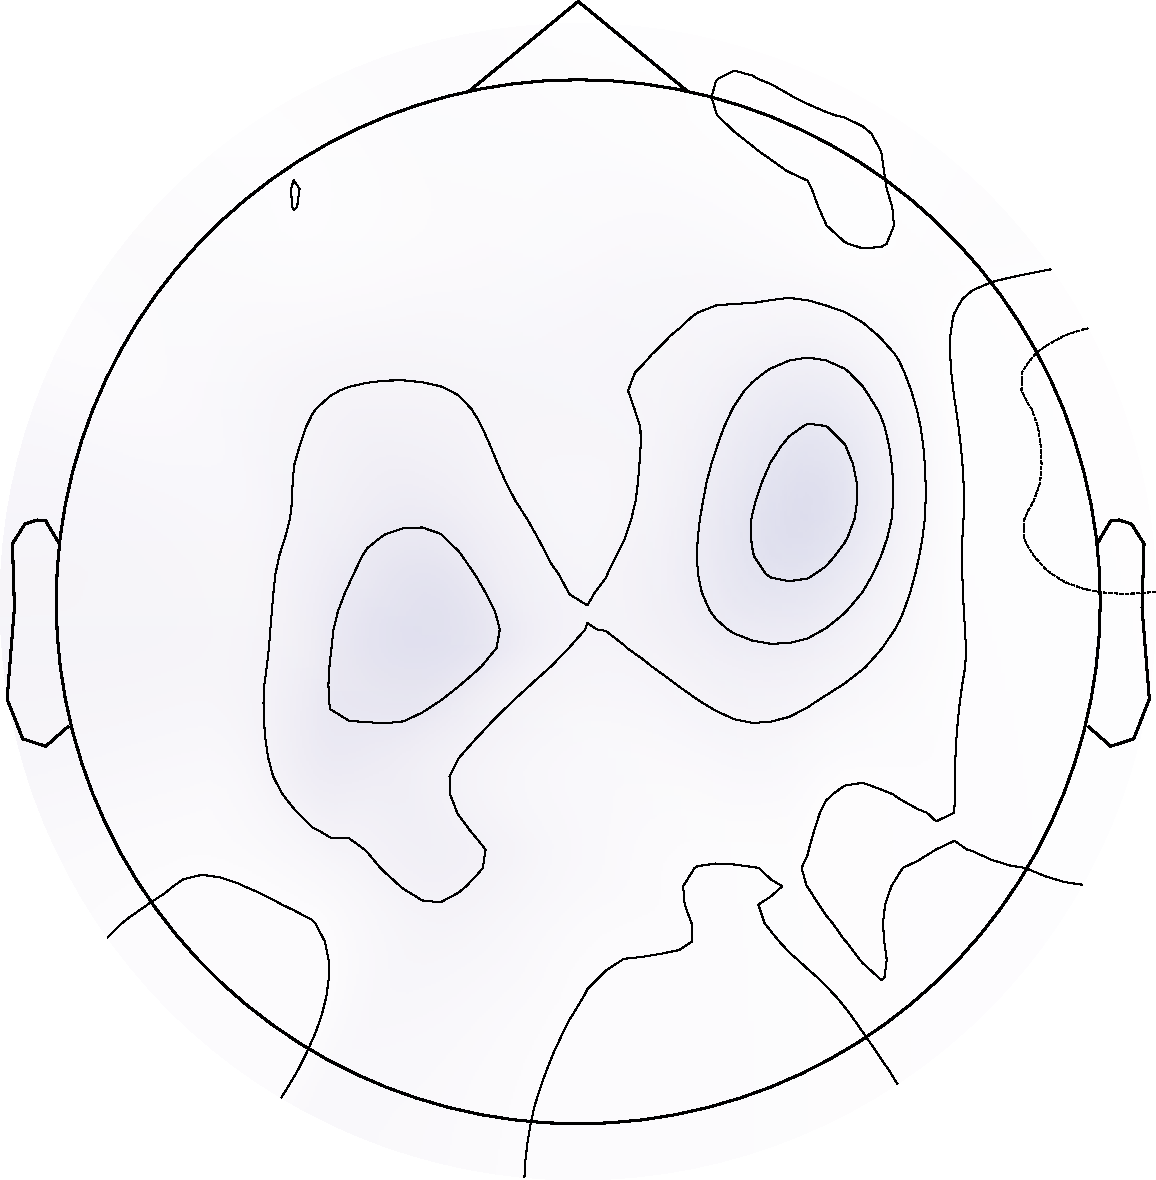
\includegraphics[width=\unitlength,page=1]{../Tesis_document/Figures/Objective_2/topoplot_bad_2.pdf}}%
    \put(0.35966985,0.97370003){\color[rgb]{0,0,0}\makebox(0,0)[lt]{\lineheight{1.25}\smash{\begin{tabular}[t]{l} \Large Fp1\end{tabular}}}}%
    \put(0.48360199,0.98294824){\color[rgb]{0,0,0}\makebox(0,0)[lt]{\lineheight{1.25}\smash{\begin{tabular}[t]{l} \Large Fpz\end{tabular}}}}%
    \put(0.60675131,0.97720749){\color[rgb]{0,0,0}\makebox(0,0)[lt]{\lineheight{1.25}\smash{\begin{tabular}[t]{l} \Large Fp2\end{tabular}}}}%
    \put(0.25167291,0.91234177){\color[rgb]{0,0,0}\makebox(0,0)[lt]{\lineheight{1.25}\smash{\begin{tabular}[t]{l} \Large AF7\end{tabular}}}}%
    \put(0.35594784,0.90619656){\color[rgb]{0,0,0}\makebox(0,0)[lt]{\lineheight{1.25}\smash{\begin{tabular}[t]{l} \Large AF3\end{tabular}}}}%
    \put(0.4842648,0.90789092){\color[rgb]{0,0,0}\makebox(0,0)[lt]{\lineheight{1.25}\smash{\begin{tabular}[t]{l} \Large AFz\end{tabular}}}}%
    \put(0.61635381,0.90817285){\color[rgb]{0,0,0}\makebox(0,0)[lt]{\lineheight{1.25}\smash{\begin{tabular}[t]{l} \Large AF4\end{tabular}}}}%
    \put(0.71557269,0.91542846){\color[rgb]{0,0,0}\makebox(0,0)[lt]{\lineheight{1.25}\smash{\begin{tabular}[t]{l} \Large AF8\end{tabular}}}}%
    \put(0.19542899,0.79852001){\color[rgb]{0,0,0}\makebox(0,0)[lt]{\lineheight{1.25}\smash{\begin{tabular}[t]{l} \Large F7\end{tabular}}}}%
    \put(0.2463776,0.79532925){\color[rgb]{0,0,0}\makebox(0,0)[lt]{\lineheight{1.25}\smash{\begin{tabular}[t]{l} \Large F5\end{tabular}}}}%
    \put(0.31178415,0.79866169){\color[rgb]{0,0,0}\makebox(0,0)[lt]{\lineheight{1.25}\smash{\begin{tabular}[t]{l} \Large F3\end{tabular}}}}%
    \put(0.3948611,0.80350183){\color[rgb]{0,0,0}\makebox(0,0)[lt]{\lineheight{1.25}\smash{\begin{tabular}[t]{l} \Large F1\end{tabular}}}}%
    \put(0.48898223,0.80600062){\color[rgb]{0,0,0}\makebox(0,0)[lt]{\lineheight{1.25}\smash{\begin{tabular}[t]{l} \Large Fz\end{tabular}}}}%
    \put(0.58636392,0.8053201){\color[rgb]{0,0,0}\makebox(0,0)[lt]{\lineheight{1.25}\smash{\begin{tabular}[t]{l} \Large F2\end{tabular}}}}%
    \put(0.66805298,0.80209838){\color[rgb]{0,0,0}\makebox(0,0)[lt]{\lineheight{1.25}\smash{\begin{tabular}[t]{l} \Large F4\end{tabular}}}}%
    \put(0.74030965,0.80128599){\color[rgb]{0,0,0}\makebox(0,0)[lt]{\lineheight{1.25}\smash{\begin{tabular}[t]{l} \Large F6\end{tabular}}}}%
    \put(0.78864244,0.80554127){\color[rgb]{0,0,0}\makebox(0,0)[lt]{\lineheight{1.25}\smash{\begin{tabular}[t]{l} \Large F8\end{tabular}}}}%
    \put(0.15454595,0.67815306){\color[rgb]{0,0,0}\makebox(0,0)[lt]{\lineheight{1.25}\smash{\begin{tabular}[t]{l} \Large FT7\end{tabular}}}}%
    \put(0.20615023,0.67997486){\color[rgb]{0,0,0}\makebox(0,0)[lt]{\lineheight{1.25}\smash{\begin{tabular}[t]{l} \Large FC5\end{tabular}}}}%
    \put(0.28304188,0.68579975){\color[rgb]{0,0,0}\makebox(0,0)[lt]{\lineheight{1.25}\smash{\begin{tabular}[t]{l} \Large FC3\end{tabular}}}}%
    \put(0.37439754,0.69273602){\color[rgb]{0,0,0}\makebox(0,0)[lt]{\lineheight{1.25}\smash{\begin{tabular}[t]{l} \Large FC1\end{tabular}}}}%
    \put(0.48466738,0.69558599){\color[rgb]{0,0,0}\makebox(0,0)[lt]{\lineheight{1.25}\smash{\begin{tabular}[t]{l} \Large FCz\end{tabular}}}}%
    \put(0.59323527,0.69300143){\color[rgb]{0,0,0}\makebox(0,0)[lt]{\lineheight{1.25}\smash{\begin{tabular}[t]{l} \Large FC2\end{tabular}}}}%
    \put(0.68863907,0.68755097){\color[rgb]{0,0,0}\makebox(0,0)[lt]{\lineheight{1.25}\smash{\begin{tabular}[t]{l} \Large FC4\end{tabular}}}}%
    \put(0.76580792,0.6824784){\color[rgb]{0,0,0}\makebox(0,0)[lt]{\lineheight{1.25}\smash{\begin{tabular}[t]{l} \Large FC6\end{tabular}}}}%
    \put(0.81263854,0.68078942){\color[rgb]{0,0,0}\makebox(0,0)[lt]{\lineheight{1.25}\smash{\begin{tabular}[t]{l} \Large FT8\end{tabular}}}}%
    \put(0.1530441,0.55517275){\color[rgb]{0,0,0}\makebox(0,0)[lt]{\lineheight{1.25}\smash{\begin{tabular}[t]{l} \Large T7\end{tabular}}}}%
    \put(0.20793166,0.56319386){\color[rgb]{0,0,0}\makebox(0,0)[lt]{\lineheight{1.25}\smash{\begin{tabular}[t]{l} \Large C5\end{tabular}}}}%
    \put(0.27584902,0.57156825){\color[rgb]{0,0,0}\makebox(0,0)[lt]{\lineheight{1.25}\smash{\begin{tabular}[t]{l} \Large C3\end{tabular}}}}%
    \put(0.37455097,0.57777021){\color[rgb]{0,0,0}\makebox(0,0)[lt]{\lineheight{1.25}\smash{\begin{tabular}[t]{l} \Large C1\end{tabular}}}}%
    \put(0.48810352,0.58059781){\color[rgb]{0,0,0}\makebox(0,0)[lt]{\lineheight{1.25}\smash{\begin{tabular}[t]{l} \Large Cz\end{tabular}}}}%
    \put(0.60220455,0.57775928){\color[rgb]{0,0,0}\makebox(0,0)[lt]{\lineheight{1.25}\smash{\begin{tabular}[t]{l} \Large C2\end{tabular}}}}%
    \put(0.70116415,0.5721481){\color[rgb]{0,0,0}\makebox(0,0)[lt]{\lineheight{1.25}\smash{\begin{tabular}[t]{l} \Large C4\end{tabular}}}}%
    \put(0.77357917,0.56454403){\color[rgb]{0,0,0}\makebox(0,0)[lt]{\lineheight{1.25}\smash{\begin{tabular}[t]{l} \Large C6\end{tabular}}}}%
    \put(0.81934775,0.55648784){\color[rgb]{0,0,0}\makebox(0,0)[lt]{\lineheight{1.25}\smash{\begin{tabular}[t]{l} \Large T8\end{tabular}}}}%
    \put(0.1517973,0.43852801){\color[rgb]{0,0,0}\makebox(0,0)[lt]{\lineheight{1.25}\smash{\begin{tabular}[t]{l} \Large TP7\end{tabular}}}}%
    \put(0.20911847,0.4508994){\color[rgb]{0,0,0}\makebox(0,0)[lt]{\lineheight{1.25}\smash{\begin{tabular}[t]{l} \Large CP5\end{tabular}}}}%
    \put(0.27925198,0.45863235){\color[rgb]{0,0,0}\makebox(0,0)[lt]{\lineheight{1.25}\smash{\begin{tabular}[t]{l} \Large CP3\end{tabular}}}}%
    \put(0.37303188,0.46333464){\color[rgb]{0,0,0}\makebox(0,0)[lt]{\lineheight{1.25}\smash{\begin{tabular}[t]{l} \Large CP1\end{tabular}}}}%
    \put(0.48386946,0.46467461){\color[rgb]{0,0,0}\makebox(0,0)[lt]{\lineheight{1.25}\smash{\begin{tabular}[t]{l} \Large CPz\end{tabular}}}}%
    \put(0.59955975,0.46310621){\color[rgb]{0,0,0}\makebox(0,0)[lt]{\lineheight{1.25}\smash{\begin{tabular}[t]{l} \Large CP2\end{tabular}}}}%
    \put(0.69365886,0.45836519){\color[rgb]{0,0,0}\makebox(0,0)[lt]{\lineheight{1.25}\smash{\begin{tabular}[t]{l} \Large CP4\end{tabular}}}}%
    \put(0.76588877,0.45053051){\color[rgb]{0,0,0}\makebox(0,0)[lt]{\lineheight{1.25}\smash{\begin{tabular}[t]{l} \Large CP6\end{tabular}}}}%
    \put(0.81109912,0.43829541){\color[rgb]{0,0,0}\makebox(0,0)[lt]{\lineheight{1.25}\smash{\begin{tabular}[t]{l} \Large TP8\end{tabular}}}}%
    \put(0.14280761,0.28880751){\color[rgb]{0,0,0}\makebox(0,0)[lt]{\lineheight{1.25}\smash{\begin{tabular}[t]{l} \Large P9\end{tabular}}}}%
    \put(0.2117726,0.33788361){\color[rgb]{0,0,0}\makebox(0,0)[lt]{\lineheight{1.25}\smash{\begin{tabular}[t]{l} \Large P7\end{tabular}}}}%
    \put(0.25524773,0.34872764){\color[rgb]{0,0,0}\makebox(0,0)[lt]{\lineheight{1.25}\smash{\begin{tabular}[t]{l} \Large P5\end{tabular}}}}%
    \put(0.31470981,0.35396111){\color[rgb]{0,0,0}\makebox(0,0)[lt]{\lineheight{1.25}\smash{\begin{tabular}[t]{l} \Large P3\end{tabular}}}}%
    \put(0.39657664,0.35639051){\color[rgb]{0,0,0}\makebox(0,0)[lt]{\lineheight{1.25}\smash{\begin{tabular}[t]{l} \Large P1\end{tabular}}}}%
    \put(0.48761791,0.35703015){\color[rgb]{0,0,0}\makebox(0,0)[lt]{\lineheight{1.25}\smash{\begin{tabular}[t]{l} \Large Pz\end{tabular}}}}%
    \put(0.58532228,0.35618991){\color[rgb]{0,0,0}\makebox(0,0)[lt]{\lineheight{1.25}\smash{\begin{tabular}[t]{l} \Large P2\end{tabular}}}}%
    \put(0.66479877,0.35384677){\color[rgb]{0,0,0}\makebox(0,0)[lt]{\lineheight{1.25}\smash{\begin{tabular}[t]{l} \Large P4\end{tabular}}}}%
    \put(0.71635297,0.34901543){\color[rgb]{0,0,0}\makebox(0,0)[lt]{\lineheight{1.25}\smash{\begin{tabular}[t]{l} \Large P6\end{tabular}}}}%
    \put(0.75830495,0.33820024){\color[rgb]{0,0,0}\makebox(0,0)[lt]{\lineheight{1.25}\smash{\begin{tabular}[t]{l} \Large P8\end{tabular}}}}%
    \put(0.82302468,0.28323031){\color[rgb]{0,0,0}\makebox(0,0)[lt]{\lineheight{1.25}\smash{\begin{tabular}[t]{l} \Large P10\end{tabular}}}}%
    \put(0.27724367,0.25345649){\color[rgb]{0,0,0}\makebox(0,0)[lt]{\lineheight{1.25}\smash{\begin{tabular}[t]{l} \Large PO7\end{tabular}}}}%
    \put(0.35847019,0.27198268){\color[rgb]{0,0,0}\makebox(0,0)[lt]{\lineheight{1.25}\smash{\begin{tabular}[t]{l} \Large PO3\end{tabular}}}}%
    \put(0.48179475,0.27697369){\color[rgb]{0,0,0}\makebox(0,0)[lt]{\lineheight{1.25}\smash{\begin{tabular}[t]{l} \Large POz\end{tabular}}}}%
    \put(0.60260385,0.27132553){\color[rgb]{0,0,0}\makebox(0,0)[lt]{\lineheight{1.25}\smash{\begin{tabular}[t]{l} \Large PO4\end{tabular}}}}%
    \put(0.68406039,0.25241987){\color[rgb]{0,0,0}\makebox(0,0)[lt]{\lineheight{1.25}\smash{\begin{tabular}[t]{l} \Large PO8\end{tabular}}}}%
    \put(0.37725394,0.20621869){\color[rgb]{0,0,0}\makebox(0,0)[lt]{\lineheight{1.25}\smash{\begin{tabular}[t]{l} \Large O1\end{tabular}}}}%
    \put(0.48447417,0.20522461){\color[rgb]{0,0,0}\makebox(0,0)[lt]{\lineheight{1.25}\smash{\begin{tabular}[t]{l} \Large Oz\end{tabular}}}}%
    \put(0.59051663,0.2072364){\color[rgb]{0,0,0}\makebox(0,0)[lt]{\lineheight{1.25}\smash{\begin{tabular}[t]{l} \Large O2\end{tabular}}}}%
    \put(0.48585855,0.1324588){\color[rgb]{0,0,0}\makebox(0,0)[lt]{\lineheight{1.25}\smash{\begin{tabular}[t]{l} \Large Iz\end{tabular}}}}%
  \end{picture}%
\endgroup%
}	
    \end{subfigure}
    \\
    \begin{subfigure}[b]{.3\linewidth}
        \centering
        \resizebox{1\linewidth}{!}{%% Creator: Inkscape 1.2.2 (b0a8486541, 2022-12-01), www.inkscape.org
%% PDF/EPS/PS + LaTeX output extension by Johan Engelen, 2010
%% Accompanies image file 'topoplot_weights_model_good_2.pdf' (pdf, eps, ps)
%%
%% To include the image in your LaTeX document, write
%%   \input{<filename>.pdf_tex}
%%  instead of
%%   \includegraphics{<filename>.pdf}
%% To scale the image, write
%%   \def\svgwidth{<desired width>}
%%   \input{<filename>.pdf_tex}
%%  instead of
%%   \includegraphics[width=<desired width>]{<filename>.pdf}
%%
%% Images with a different path to the parent latex file can
%% be accessed with the `import' package (which may need to be
%% installed) using
%%   \usepackage{import}
%% in the preamble, and then including the image with
%%   \import{<path to file>}{<filename>.pdf_tex}
%% Alternatively, one can specify
%%   \graphicspath{{<path to file>/}}
%% 
%% For more information, please see info/svg-inkscape on CTAN:
%%   http://tug.ctan.org/tex-archive/info/svg-inkscape
%%
\begingroup%
  \makeatletter%
  \providecommand\color[2][]{%
    \errmessage{(Inkscape) Color is used for the text in Inkscape, but the package 'color.sty' is not loaded}%
    \renewcommand\color[2][]{}%
  }%
  \providecommand\transparent[1]{%
    \errmessage{(Inkscape) Transparency is used (non-zero) for the text in Inkscape, but the package 'transparent.sty' is not loaded}%
    \renewcommand\transparent[1]{}%
  }%
  \providecommand\rotatebox[2]{#2}%
  \newcommand*\fsize{\dimexpr\f@size pt\relax}%
  \newcommand*\lineheight[1]{\fontsize{\fsize}{#1\fsize}\selectfont}%
  \ifx\svgwidth\undefined%
    \setlength{\unitlength}{555.0933117bp}%
    \ifx\svgscale\undefined%
      \relax%
    \else%
      \setlength{\unitlength}{\unitlength * \real{\svgscale}}%
    \fi%
  \else%
    \setlength{\unitlength}{\svgwidth}%
  \fi%
  \global\let\svgwidth\undefined%
  \global\let\svgscale\undefined%
  \makeatother%
  \begin{picture}(1,1.0200345)%
    \lineheight{1}%
    \setlength\tabcolsep{0pt}%
    \put(0,0){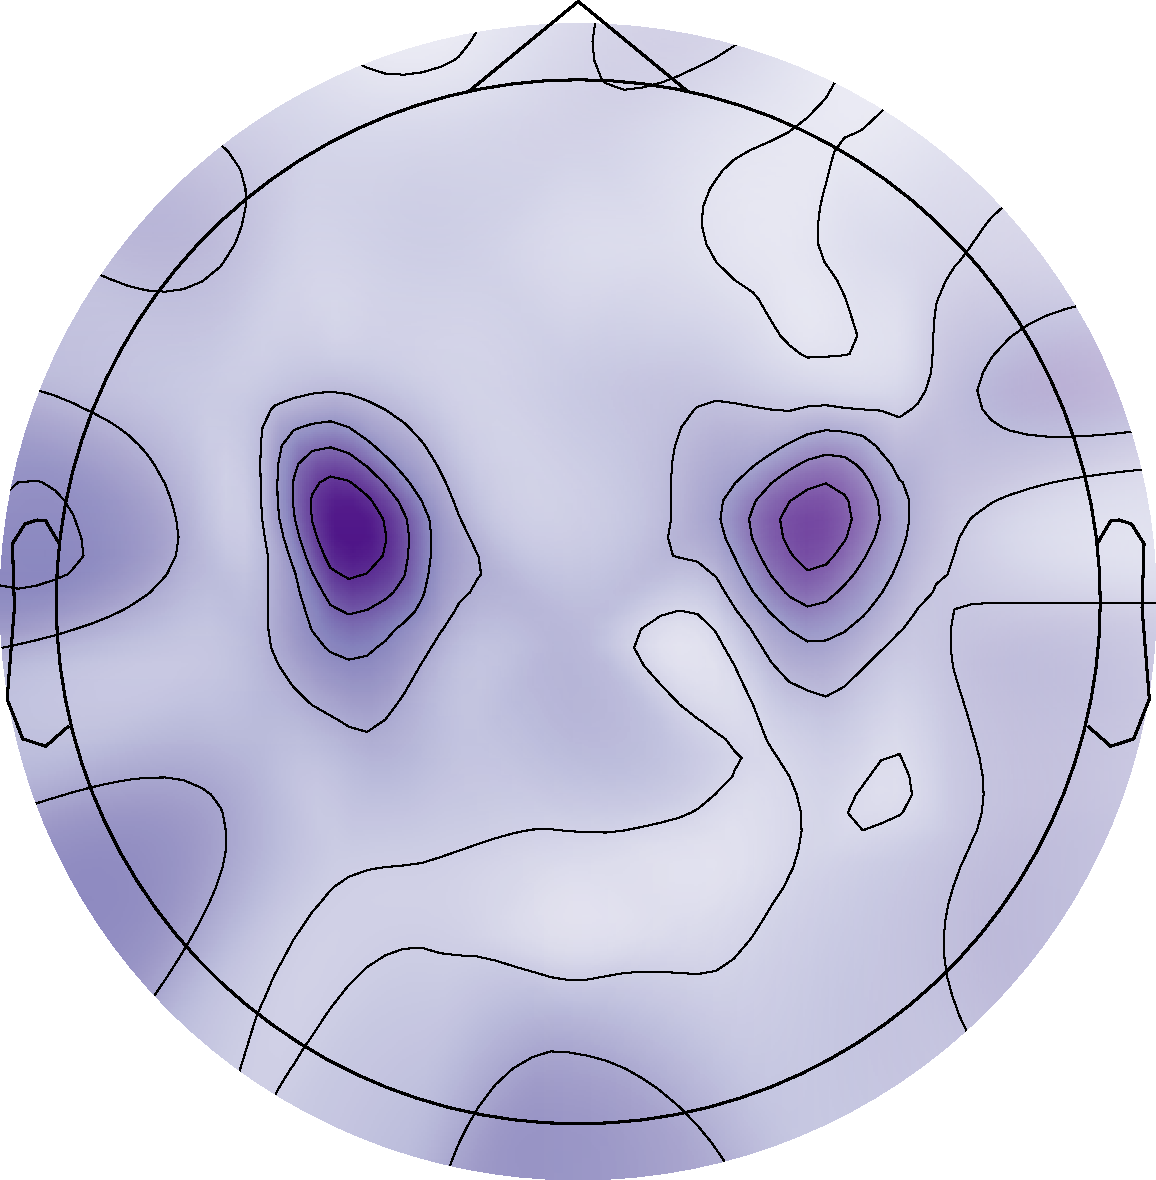
\includegraphics[width=\unitlength,page=1]{../Tesis_document/Figures/Objective_2/topoplot_weights_model_good_2.pdf}}%
    \put(0.35967082,0.97370064){\color[rgb]{0,0,0}\makebox(0,0)[lt]{\lineheight{1.25}\smash{\begin{tabular}[t]{l} \Large Fp1\end{tabular}}}}%
    \put(0.48360304,0.98294885){\color[rgb]{0,0,0}\makebox(0,0)[lt]{\lineheight{1.25}\smash{\begin{tabular}[t]{l} \Large Fpz\end{tabular}}}}%
    \put(0.60675244,0.9772081){\color[rgb]{0,0,0}\makebox(0,0)[lt]{\lineheight{1.25}\smash{\begin{tabular}[t]{l} \Large Fp2\end{tabular}}}}%
    \put(0.25167381,0.91234234){\color[rgb]{0,0,0}\makebox(0,0)[lt]{\lineheight{1.25}\smash{\begin{tabular}[t]{l} \Large AF7\end{tabular}}}}%
    \put(0.35594882,0.90619712){\color[rgb]{0,0,0}\makebox(0,0)[lt]{\lineheight{1.25}\smash{\begin{tabular}[t]{l} \Large AF3\end{tabular}}}}%
    \put(0.48426585,0.90789149){\color[rgb]{0,0,0}\makebox(0,0)[lt]{\lineheight{1.25}\smash{\begin{tabular}[t]{l} \Large AFz\end{tabular}}}}%
    \put(0.61635495,0.90817342){\color[rgb]{0,0,0}\makebox(0,0)[lt]{\lineheight{1.25}\smash{\begin{tabular}[t]{l} \Large AF4\end{tabular}}}}%
    \put(0.71557388,0.91542903){\color[rgb]{0,0,0}\makebox(0,0)[lt]{\lineheight{1.25}\smash{\begin{tabular}[t]{l} \Large AF8\end{tabular}}}}%
    \put(0.19542987,0.7985205){\color[rgb]{0,0,0}\makebox(0,0)[lt]{\lineheight{1.25}\smash{\begin{tabular}[t]{l} \Large F7\end{tabular}}}}%
    \put(0.24637851,0.79532974){\color[rgb]{0,0,0}\makebox(0,0)[lt]{\lineheight{1.25}\smash{\begin{tabular}[t]{l} \Large F5\end{tabular}}}}%
    \put(0.31178509,0.79866219){\color[rgb]{0,0,0}\makebox(0,0)[lt]{\lineheight{1.25}\smash{\begin{tabular}[t]{l} \Large F3\end{tabular}}}}%
    \put(0.39486209,0.80350233){\color[rgb]{0,0,0}\makebox(0,0)[lt]{\lineheight{1.25}\smash{\begin{tabular}[t]{l} \Large F1\end{tabular}}}}%
    \put(0.48898329,0.80600112){\color[rgb]{0,0,0}\makebox(0,0)[lt]{\lineheight{1.25}\smash{\begin{tabular}[t]{l} \Large Fz\end{tabular}}}}%
    \put(0.58636504,0.8053206){\color[rgb]{0,0,0}\makebox(0,0)[lt]{\lineheight{1.25}\smash{\begin{tabular}[t]{l} \Large F2\end{tabular}}}}%
    \put(0.66805415,0.80209888){\color[rgb]{0,0,0}\makebox(0,0)[lt]{\lineheight{1.25}\smash{\begin{tabular}[t]{l} \Large F4\end{tabular}}}}%
    \put(0.74031086,0.80128649){\color[rgb]{0,0,0}\makebox(0,0)[lt]{\lineheight{1.25}\smash{\begin{tabular}[t]{l} \Large F6\end{tabular}}}}%
    \put(0.78864369,0.80554177){\color[rgb]{0,0,0}\makebox(0,0)[lt]{\lineheight{1.25}\smash{\begin{tabular}[t]{l} \Large F8\end{tabular}}}}%
    \put(0.1545468,0.67815348){\color[rgb]{0,0,0}\makebox(0,0)[lt]{\lineheight{1.25}\smash{\begin{tabular}[t]{l} \Large FT7\end{tabular}}}}%
    \put(0.20615111,0.67997528){\color[rgb]{0,0,0}\makebox(0,0)[lt]{\lineheight{1.25}\smash{\begin{tabular}[t]{l} \Large FC5\end{tabular}}}}%
    \put(0.28304281,0.68580018){\color[rgb]{0,0,0}\makebox(0,0)[lt]{\lineheight{1.25}\smash{\begin{tabular}[t]{l} \Large FC3\end{tabular}}}}%
    \put(0.37439852,0.69273645){\color[rgb]{0,0,0}\makebox(0,0)[lt]{\lineheight{1.25}\smash{\begin{tabular}[t]{l} \Large FC1\end{tabular}}}}%
    \put(0.48466843,0.69558642){\color[rgb]{0,0,0}\makebox(0,0)[lt]{\lineheight{1.25}\smash{\begin{tabular}[t]{l} \Large FCz\end{tabular}}}}%
    \put(0.59323639,0.69300187){\color[rgb]{0,0,0}\makebox(0,0)[lt]{\lineheight{1.25}\smash{\begin{tabular}[t]{l} \Large FC2\end{tabular}}}}%
    \put(0.68864025,0.68755139){\color[rgb]{0,0,0}\makebox(0,0)[lt]{\lineheight{1.25}\smash{\begin{tabular}[t]{l} \Large FC4\end{tabular}}}}%
    \put(0.76580915,0.68247882){\color[rgb]{0,0,0}\makebox(0,0)[lt]{\lineheight{1.25}\smash{\begin{tabular}[t]{l} \Large FC6\end{tabular}}}}%
    \put(0.81263979,0.68078985){\color[rgb]{0,0,0}\makebox(0,0)[lt]{\lineheight{1.25}\smash{\begin{tabular}[t]{l} \Large FT8\end{tabular}}}}%
    \put(0.15304494,0.55517309){\color[rgb]{0,0,0}\makebox(0,0)[lt]{\lineheight{1.25}\smash{\begin{tabular}[t]{l} \Large T7\end{tabular}}}}%
    \put(0.20793254,0.56319421){\color[rgb]{0,0,0}\makebox(0,0)[lt]{\lineheight{1.25}\smash{\begin{tabular}[t]{l} \Large C5\end{tabular}}}}%
    \put(0.27584995,0.57156861){\color[rgb]{0,0,0}\makebox(0,0)[lt]{\lineheight{1.25}\smash{\begin{tabular}[t]{l} \Large C3\end{tabular}}}}%
    \put(0.37455196,0.57777057){\color[rgb]{0,0,0}\makebox(0,0)[lt]{\lineheight{1.25}\smash{\begin{tabular}[t]{l} \Large C1\end{tabular}}}}%
    \put(0.48810457,0.58059817){\color[rgb]{0,0,0}\makebox(0,0)[lt]{\lineheight{1.25}\smash{\begin{tabular}[t]{l} \Large Cz\end{tabular}}}}%
    \put(0.60220567,0.57775964){\color[rgb]{0,0,0}\makebox(0,0)[lt]{\lineheight{1.25}\smash{\begin{tabular}[t]{l} \Large C2\end{tabular}}}}%
    \put(0.70116534,0.57214845){\color[rgb]{0,0,0}\makebox(0,0)[lt]{\lineheight{1.25}\smash{\begin{tabular}[t]{l} \Large C4\end{tabular}}}}%
    \put(0.7735804,0.56454438){\color[rgb]{0,0,0}\makebox(0,0)[lt]{\lineheight{1.25}\smash{\begin{tabular}[t]{l} \Large C6\end{tabular}}}}%
    \put(0.81934901,0.55648819){\color[rgb]{0,0,0}\makebox(0,0)[lt]{\lineheight{1.25}\smash{\begin{tabular}[t]{l} \Large T8\end{tabular}}}}%
    \put(0.15179814,0.43852829){\color[rgb]{0,0,0}\makebox(0,0)[lt]{\lineheight{1.25}\smash{\begin{tabular}[t]{l} \Large TP7\end{tabular}}}}%
    \put(0.20911935,0.45089969){\color[rgb]{0,0,0}\makebox(0,0)[lt]{\lineheight{1.25}\smash{\begin{tabular}[t]{l} \Large CP5\end{tabular}}}}%
    \put(0.2792529,0.45863264){\color[rgb]{0,0,0}\makebox(0,0)[lt]{\lineheight{1.25}\smash{\begin{tabular}[t]{l} \Large CP3\end{tabular}}}}%
    \put(0.37303286,0.46333493){\color[rgb]{0,0,0}\makebox(0,0)[lt]{\lineheight{1.25}\smash{\begin{tabular}[t]{l} \Large CP1\end{tabular}}}}%
    \put(0.48387051,0.4646749){\color[rgb]{0,0,0}\makebox(0,0)[lt]{\lineheight{1.25}\smash{\begin{tabular}[t]{l} \Large CPz\end{tabular}}}}%
    \put(0.59956087,0.4631065){\color[rgb]{0,0,0}\makebox(0,0)[lt]{\lineheight{1.25}\smash{\begin{tabular}[t]{l} \Large CP2\end{tabular}}}}%
    \put(0.69366004,0.45836548){\color[rgb]{0,0,0}\makebox(0,0)[lt]{\lineheight{1.25}\smash{\begin{tabular}[t]{l} \Large CP4\end{tabular}}}}%
    \put(0.76589,0.45053079){\color[rgb]{0,0,0}\makebox(0,0)[lt]{\lineheight{1.25}\smash{\begin{tabular}[t]{l} \Large CP6\end{tabular}}}}%
    \put(0.81110038,0.43829568){\color[rgb]{0,0,0}\makebox(0,0)[lt]{\lineheight{1.25}\smash{\begin{tabular}[t]{l} \Large TP8\end{tabular}}}}%
    \put(0.14280845,0.28880769){\color[rgb]{0,0,0}\makebox(0,0)[lt]{\lineheight{1.25}\smash{\begin{tabular}[t]{l} \Large P9\end{tabular}}}}%
    \put(0.21177348,0.33788382){\color[rgb]{0,0,0}\makebox(0,0)[lt]{\lineheight{1.25}\smash{\begin{tabular}[t]{l} \Large P7\end{tabular}}}}%
    \put(0.25524864,0.34872785){\color[rgb]{0,0,0}\makebox(0,0)[lt]{\lineheight{1.25}\smash{\begin{tabular}[t]{l} \Large P5\end{tabular}}}}%
    \put(0.31471076,0.35396133){\color[rgb]{0,0,0}\makebox(0,0)[lt]{\lineheight{1.25}\smash{\begin{tabular}[t]{l} \Large P3\end{tabular}}}}%
    \put(0.39657764,0.35639073){\color[rgb]{0,0,0}\makebox(0,0)[lt]{\lineheight{1.25}\smash{\begin{tabular}[t]{l} \Large P1\end{tabular}}}}%
    \put(0.48761896,0.35703037){\color[rgb]{0,0,0}\makebox(0,0)[lt]{\lineheight{1.25}\smash{\begin{tabular}[t]{l} \Large Pz\end{tabular}}}}%
    \put(0.58532339,0.35619013){\color[rgb]{0,0,0}\makebox(0,0)[lt]{\lineheight{1.25}\smash{\begin{tabular}[t]{l} \Large P2\end{tabular}}}}%
    \put(0.66479994,0.35384699){\color[rgb]{0,0,0}\makebox(0,0)[lt]{\lineheight{1.25}\smash{\begin{tabular}[t]{l} \Large P4\end{tabular}}}}%
    \put(0.71635417,0.34901564){\color[rgb]{0,0,0}\makebox(0,0)[lt]{\lineheight{1.25}\smash{\begin{tabular}[t]{l} \Large P6\end{tabular}}}}%
    \put(0.75830618,0.33820045){\color[rgb]{0,0,0}\makebox(0,0)[lt]{\lineheight{1.25}\smash{\begin{tabular}[t]{l} \Large P8\end{tabular}}}}%
    \put(0.82302594,0.28323049){\color[rgb]{0,0,0}\makebox(0,0)[lt]{\lineheight{1.25}\smash{\begin{tabular}[t]{l} \Large P10\end{tabular}}}}%
    \put(0.27724459,0.25345665){\color[rgb]{0,0,0}\makebox(0,0)[lt]{\lineheight{1.25}\smash{\begin{tabular}[t]{l} \Large PO7\end{tabular}}}}%
    \put(0.35847117,0.27198285){\color[rgb]{0,0,0}\makebox(0,0)[lt]{\lineheight{1.25}\smash{\begin{tabular}[t]{l} \Large PO3\end{tabular}}}}%
    \put(0.4817958,0.27697386){\color[rgb]{0,0,0}\makebox(0,0)[lt]{\lineheight{1.25}\smash{\begin{tabular}[t]{l} \Large POz\end{tabular}}}}%
    \put(0.60260497,0.2713257){\color[rgb]{0,0,0}\makebox(0,0)[lt]{\lineheight{1.25}\smash{\begin{tabular}[t]{l} \Large PO4\end{tabular}}}}%
    \put(0.68406156,0.25242003){\color[rgb]{0,0,0}\makebox(0,0)[lt]{\lineheight{1.25}\smash{\begin{tabular}[t]{l} \Large PO8\end{tabular}}}}%
    \put(0.37725493,0.20621882){\color[rgb]{0,0,0}\makebox(0,0)[lt]{\lineheight{1.25}\smash{\begin{tabular}[t]{l} \Large O1\end{tabular}}}}%
    \put(0.48447522,0.20522474){\color[rgb]{0,0,0}\makebox(0,0)[lt]{\lineheight{1.25}\smash{\begin{tabular}[t]{l} \Large Oz\end{tabular}}}}%
    \put(0.59051775,0.20723652){\color[rgb]{0,0,0}\makebox(0,0)[lt]{\lineheight{1.25}\smash{\begin{tabular}[t]{l} \Large O2\end{tabular}}}}%
    \put(0.4858596,0.13245888){\color[rgb]{0,0,0}\makebox(0,0)[lt]{\lineheight{1.25}\smash{\begin{tabular}[t]{l} \Large Iz\end{tabular}}}}%
  \end{picture}%
\endgroup%
}	
    \end{subfigure}
    ~ 
    \begin{subfigure}[b]{.3\linewidth}
        \centering
        \resizebox{1\linewidth}{!}{%% Creator: Inkscape 1.2.2 (b0a8486541, 2022-12-01), www.inkscape.org
%% PDF/EPS/PS + LaTeX output extension by Johan Engelen, 2010
%% Accompanies image file 'topoplot_weights_model_medium_2.pdf' (pdf, eps, ps)
%%
%% To include the image in your LaTeX document, write
%%   \input{<filename>.pdf_tex}
%%  instead of
%%   \includegraphics{<filename>.pdf}
%% To scale the image, write
%%   \def\svgwidth{<desired width>}
%%   \input{<filename>.pdf_tex}
%%  instead of
%%   \includegraphics[width=<desired width>]{<filename>.pdf}
%%
%% Images with a different path to the parent latex file can
%% be accessed with the `import' package (which may need to be
%% installed) using
%%   \usepackage{import}
%% in the preamble, and then including the image with
%%   \import{<path to file>}{<filename>.pdf_tex}
%% Alternatively, one can specify
%%   \graphicspath{{<path to file>/}}
%% 
%% For more information, please see info/svg-inkscape on CTAN:
%%   http://tug.ctan.org/tex-archive/info/svg-inkscape
%%
\begingroup%
  \makeatletter%
  \providecommand\color[2][]{%
    \errmessage{(Inkscape) Color is used for the text in Inkscape, but the package 'color.sty' is not loaded}%
    \renewcommand\color[2][]{}%
  }%
  \providecommand\transparent[1]{%
    \errmessage{(Inkscape) Transparency is used (non-zero) for the text in Inkscape, but the package 'transparent.sty' is not loaded}%
    \renewcommand\transparent[1]{}%
  }%
  \providecommand\rotatebox[2]{#2}%
  \newcommand*\fsize{\dimexpr\f@size pt\relax}%
  \newcommand*\lineheight[1]{\fontsize{\fsize}{#1\fsize}\selectfont}%
  \ifx\svgwidth\undefined%
    \setlength{\unitlength}{555.0933117bp}%
    \ifx\svgscale\undefined%
      \relax%
    \else%
      \setlength{\unitlength}{\unitlength * \real{\svgscale}}%
    \fi%
  \else%
    \setlength{\unitlength}{\svgwidth}%
  \fi%
  \global\let\svgwidth\undefined%
  \global\let\svgscale\undefined%
  \makeatother%
  \begin{picture}(1,1.0200345)%
    \lineheight{1}%
    \setlength\tabcolsep{0pt}%
    \put(0,0){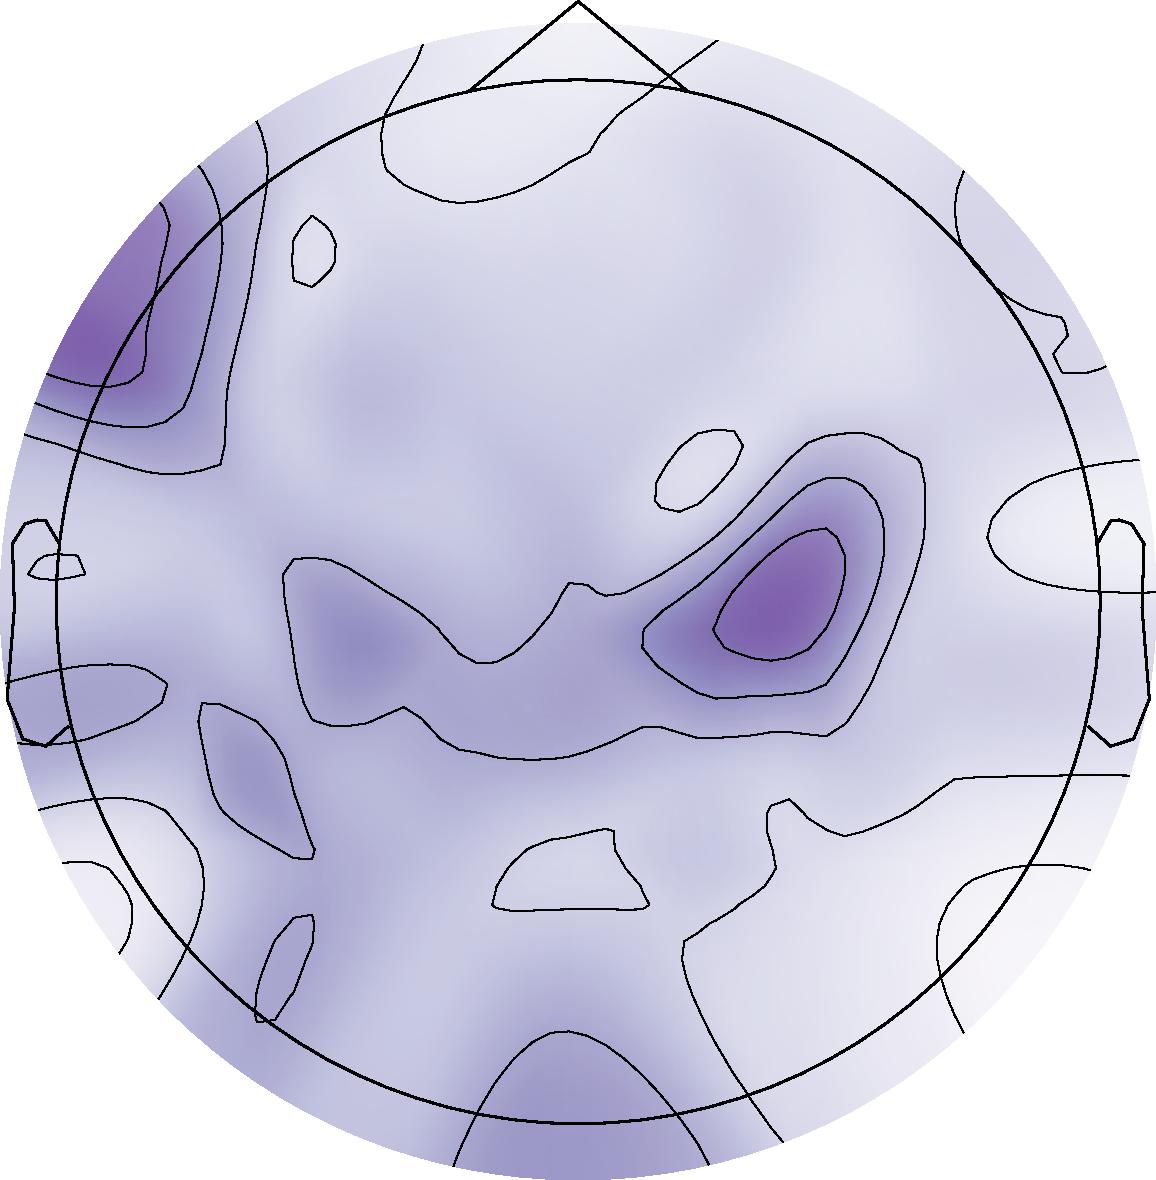
\includegraphics[width=\unitlength,page=1]{../Tesis_document/Figures/Objective_2/topoplot_weights_model_medium_2.pdf}}%
    \put(0.35967023,0.97370064){\color[rgb]{0,0,0}\makebox(0,0)[lt]{\lineheight{1.25}\smash{\begin{tabular}[t]{l} \Large Fp1\end{tabular}}}}%
    \put(0.48360245,0.98294885){\color[rgb]{0,0,0}\makebox(0,0)[lt]{\lineheight{1.25}\smash{\begin{tabular}[t]{l} \Large Fpz\end{tabular}}}}%
    \put(0.60675185,0.9772081){\color[rgb]{0,0,0}\makebox(0,0)[lt]{\lineheight{1.25}\smash{\begin{tabular}[t]{l} \Large Fp2\end{tabular}}}}%
    \put(0.25167322,0.91234234){\color[rgb]{0,0,0}\makebox(0,0)[lt]{\lineheight{1.25}\smash{\begin{tabular}[t]{l} \Large AF7\end{tabular}}}}%
    \put(0.35594822,0.90619712){\color[rgb]{0,0,0}\makebox(0,0)[lt]{\lineheight{1.25}\smash{\begin{tabular}[t]{l} \Large AF3\end{tabular}}}}%
    \put(0.48426526,0.90789149){\color[rgb]{0,0,0}\makebox(0,0)[lt]{\lineheight{1.25}\smash{\begin{tabular}[t]{l} \Large AFz\end{tabular}}}}%
    \put(0.61635436,0.90817342){\color[rgb]{0,0,0}\makebox(0,0)[lt]{\lineheight{1.25}\smash{\begin{tabular}[t]{l} \Large AF4\end{tabular}}}}%
    \put(0.71557329,0.91542903){\color[rgb]{0,0,0}\makebox(0,0)[lt]{\lineheight{1.25}\smash{\begin{tabular}[t]{l} \Large AF8\end{tabular}}}}%
    \put(0.19542927,0.7985205){\color[rgb]{0,0,0}\makebox(0,0)[lt]{\lineheight{1.25}\smash{\begin{tabular}[t]{l} \Large F7\end{tabular}}}}%
    \put(0.24637791,0.79532974){\color[rgb]{0,0,0}\makebox(0,0)[lt]{\lineheight{1.25}\smash{\begin{tabular}[t]{l} \Large F5\end{tabular}}}}%
    \put(0.3117845,0.79866219){\color[rgb]{0,0,0}\makebox(0,0)[lt]{\lineheight{1.25}\smash{\begin{tabular}[t]{l} \Large F3\end{tabular}}}}%
    \put(0.3948615,0.80350233){\color[rgb]{0,0,0}\makebox(0,0)[lt]{\lineheight{1.25}\smash{\begin{tabular}[t]{l} \Large F1\end{tabular}}}}%
    \put(0.4889827,0.80600112){\color[rgb]{0,0,0}\makebox(0,0)[lt]{\lineheight{1.25}\smash{\begin{tabular}[t]{l} \Large Fz\end{tabular}}}}%
    \put(0.58636445,0.8053206){\color[rgb]{0,0,0}\makebox(0,0)[lt]{\lineheight{1.25}\smash{\begin{tabular}[t]{l} \Large F2\end{tabular}}}}%
    \put(0.66805355,0.80209888){\color[rgb]{0,0,0}\makebox(0,0)[lt]{\lineheight{1.25}\smash{\begin{tabular}[t]{l} \Large F4\end{tabular}}}}%
    \put(0.74031027,0.80128649){\color[rgb]{0,0,0}\makebox(0,0)[lt]{\lineheight{1.25}\smash{\begin{tabular}[t]{l} \Large F6\end{tabular}}}}%
    \put(0.78864309,0.80554177){\color[rgb]{0,0,0}\makebox(0,0)[lt]{\lineheight{1.25}\smash{\begin{tabular}[t]{l} \Large F8\end{tabular}}}}%
    \put(0.1545462,0.67815348){\color[rgb]{0,0,0}\makebox(0,0)[lt]{\lineheight{1.25}\smash{\begin{tabular}[t]{l} \Large FT7\end{tabular}}}}%
    \put(0.20615052,0.67997528){\color[rgb]{0,0,0}\makebox(0,0)[lt]{\lineheight{1.25}\smash{\begin{tabular}[t]{l} \Large FC5\end{tabular}}}}%
    \put(0.28304222,0.68580018){\color[rgb]{0,0,0}\makebox(0,0)[lt]{\lineheight{1.25}\smash{\begin{tabular}[t]{l} \Large FC3\end{tabular}}}}%
    \put(0.37439793,0.69273645){\color[rgb]{0,0,0}\makebox(0,0)[lt]{\lineheight{1.25}\smash{\begin{tabular}[t]{l} \Large FC1\end{tabular}}}}%
    \put(0.48466784,0.69558642){\color[rgb]{0,0,0}\makebox(0,0)[lt]{\lineheight{1.25}\smash{\begin{tabular}[t]{l} \Large FCz\end{tabular}}}}%
    \put(0.5932358,0.69300187){\color[rgb]{0,0,0}\makebox(0,0)[lt]{\lineheight{1.25}\smash{\begin{tabular}[t]{l} \Large FC2\end{tabular}}}}%
    \put(0.68863966,0.68755139){\color[rgb]{0,0,0}\makebox(0,0)[lt]{\lineheight{1.25}\smash{\begin{tabular}[t]{l} \Large FC4\end{tabular}}}}%
    \put(0.76580856,0.68247882){\color[rgb]{0,0,0}\makebox(0,0)[lt]{\lineheight{1.25}\smash{\begin{tabular}[t]{l} \Large FC6\end{tabular}}}}%
    \put(0.8126392,0.68078985){\color[rgb]{0,0,0}\makebox(0,0)[lt]{\lineheight{1.25}\smash{\begin{tabular}[t]{l} \Large FT8\end{tabular}}}}%
    \put(0.15304435,0.55517309){\color[rgb]{0,0,0}\makebox(0,0)[lt]{\lineheight{1.25}\smash{\begin{tabular}[t]{l} \Large T7\end{tabular}}}}%
    \put(0.20793195,0.56319421){\color[rgb]{0,0,0}\makebox(0,0)[lt]{\lineheight{1.25}\smash{\begin{tabular}[t]{l} \Large C5\end{tabular}}}}%
    \put(0.27584935,0.57156861){\color[rgb]{0,0,0}\makebox(0,0)[lt]{\lineheight{1.25}\smash{\begin{tabular}[t]{l} \Large C3\end{tabular}}}}%
    \put(0.37455137,0.57777057){\color[rgb]{0,0,0}\makebox(0,0)[lt]{\lineheight{1.25}\smash{\begin{tabular}[t]{l} \Large C1\end{tabular}}}}%
    \put(0.48810398,0.58059817){\color[rgb]{0,0,0}\makebox(0,0)[lt]{\lineheight{1.25}\smash{\begin{tabular}[t]{l} \Large Cz\end{tabular}}}}%
    \put(0.60220508,0.57775964){\color[rgb]{0,0,0}\makebox(0,0)[lt]{\lineheight{1.25}\smash{\begin{tabular}[t]{l} \Large C2\end{tabular}}}}%
    \put(0.70116474,0.57214845){\color[rgb]{0,0,0}\makebox(0,0)[lt]{\lineheight{1.25}\smash{\begin{tabular}[t]{l} \Large C4\end{tabular}}}}%
    \put(0.77357981,0.56454438){\color[rgb]{0,0,0}\makebox(0,0)[lt]{\lineheight{1.25}\smash{\begin{tabular}[t]{l} \Large C6\end{tabular}}}}%
    \put(0.81934842,0.55648819){\color[rgb]{0,0,0}\makebox(0,0)[lt]{\lineheight{1.25}\smash{\begin{tabular}[t]{l} \Large T8\end{tabular}}}}%
    \put(0.15179755,0.43852829){\color[rgb]{0,0,0}\makebox(0,0)[lt]{\lineheight{1.25}\smash{\begin{tabular}[t]{l} \Large TP7\end{tabular}}}}%
    \put(0.20911876,0.45089969){\color[rgb]{0,0,0}\makebox(0,0)[lt]{\lineheight{1.25}\smash{\begin{tabular}[t]{l} \Large CP5\end{tabular}}}}%
    \put(0.27925231,0.45863264){\color[rgb]{0,0,0}\makebox(0,0)[lt]{\lineheight{1.25}\smash{\begin{tabular}[t]{l} \Large CP3\end{tabular}}}}%
    \put(0.37303227,0.46333493){\color[rgb]{0,0,0}\makebox(0,0)[lt]{\lineheight{1.25}\smash{\begin{tabular}[t]{l} \Large CP1\end{tabular}}}}%
    \put(0.48386992,0.4646749){\color[rgb]{0,0,0}\makebox(0,0)[lt]{\lineheight{1.25}\smash{\begin{tabular}[t]{l} \Large CPz\end{tabular}}}}%
    \put(0.59956028,0.4631065){\color[rgb]{0,0,0}\makebox(0,0)[lt]{\lineheight{1.25}\smash{\begin{tabular}[t]{l} \Large CP2\end{tabular}}}}%
    \put(0.69365945,0.45836548){\color[rgb]{0,0,0}\makebox(0,0)[lt]{\lineheight{1.25}\smash{\begin{tabular}[t]{l} \Large CP4\end{tabular}}}}%
    \put(0.76588941,0.45053079){\color[rgb]{0,0,0}\makebox(0,0)[lt]{\lineheight{1.25}\smash{\begin{tabular}[t]{l} \Large CP6\end{tabular}}}}%
    \put(0.81109979,0.43829568){\color[rgb]{0,0,0}\makebox(0,0)[lt]{\lineheight{1.25}\smash{\begin{tabular}[t]{l} \Large TP8\end{tabular}}}}%
    \put(0.14280785,0.28880769){\color[rgb]{0,0,0}\makebox(0,0)[lt]{\lineheight{1.25}\smash{\begin{tabular}[t]{l} \Large P9\end{tabular}}}}%
    \put(0.21177289,0.33788382){\color[rgb]{0,0,0}\makebox(0,0)[lt]{\lineheight{1.25}\smash{\begin{tabular}[t]{l} \Large P7\end{tabular}}}}%
    \put(0.25524804,0.34872785){\color[rgb]{0,0,0}\makebox(0,0)[lt]{\lineheight{1.25}\smash{\begin{tabular}[t]{l} \Large P5\end{tabular}}}}%
    \put(0.31471017,0.35396133){\color[rgb]{0,0,0}\makebox(0,0)[lt]{\lineheight{1.25}\smash{\begin{tabular}[t]{l} \Large P3\end{tabular}}}}%
    \put(0.39657705,0.35639073){\color[rgb]{0,0,0}\makebox(0,0)[lt]{\lineheight{1.25}\smash{\begin{tabular}[t]{l} \Large P1\end{tabular}}}}%
    \put(0.48761837,0.35703037){\color[rgb]{0,0,0}\makebox(0,0)[lt]{\lineheight{1.25}\smash{\begin{tabular}[t]{l} \Large Pz\end{tabular}}}}%
    \put(0.5853228,0.35619013){\color[rgb]{0,0,0}\makebox(0,0)[lt]{\lineheight{1.25}\smash{\begin{tabular}[t]{l} \Large P2\end{tabular}}}}%
    \put(0.66479935,0.35384699){\color[rgb]{0,0,0}\makebox(0,0)[lt]{\lineheight{1.25}\smash{\begin{tabular}[t]{l} \Large P4\end{tabular}}}}%
    \put(0.71635358,0.34901564){\color[rgb]{0,0,0}\makebox(0,0)[lt]{\lineheight{1.25}\smash{\begin{tabular}[t]{l} \Large P6\end{tabular}}}}%
    \put(0.75830558,0.33820045){\color[rgb]{0,0,0}\makebox(0,0)[lt]{\lineheight{1.25}\smash{\begin{tabular}[t]{l} \Large P8\end{tabular}}}}%
    \put(0.82302535,0.28323049){\color[rgb]{0,0,0}\makebox(0,0)[lt]{\lineheight{1.25}\smash{\begin{tabular}[t]{l} \Large P10\end{tabular}}}}%
    \put(0.277244,0.25345665){\color[rgb]{0,0,0}\makebox(0,0)[lt]{\lineheight{1.25}\smash{\begin{tabular}[t]{l} \Large PO7\end{tabular}}}}%
    \put(0.35847058,0.27198285){\color[rgb]{0,0,0}\makebox(0,0)[lt]{\lineheight{1.25}\smash{\begin{tabular}[t]{l} \Large PO3\end{tabular}}}}%
    \put(0.4817952,0.27697386){\color[rgb]{0,0,0}\makebox(0,0)[lt]{\lineheight{1.25}\smash{\begin{tabular}[t]{l} \Large POz\end{tabular}}}}%
    \put(0.60260438,0.2713257){\color[rgb]{0,0,0}\makebox(0,0)[lt]{\lineheight{1.25}\smash{\begin{tabular}[t]{l} \Large PO4\end{tabular}}}}%
    \put(0.68406097,0.25242003){\color[rgb]{0,0,0}\makebox(0,0)[lt]{\lineheight{1.25}\smash{\begin{tabular}[t]{l} \Large PO8\end{tabular}}}}%
    \put(0.37725433,0.20621882){\color[rgb]{0,0,0}\makebox(0,0)[lt]{\lineheight{1.25}\smash{\begin{tabular}[t]{l} \Large O1\end{tabular}}}}%
    \put(0.48447463,0.20522474){\color[rgb]{0,0,0}\makebox(0,0)[lt]{\lineheight{1.25}\smash{\begin{tabular}[t]{l} \Large Oz\end{tabular}}}}%
    \put(0.59051715,0.20723652){\color[rgb]{0,0,0}\makebox(0,0)[lt]{\lineheight{1.25}\smash{\begin{tabular}[t]{l} \Large O2\end{tabular}}}}%
    \put(0.48585901,0.13245888){\color[rgb]{0,0,0}\makebox(0,0)[lt]{\lineheight{1.25}\smash{\begin{tabular}[t]{l} \Large Iz\end{tabular}}}}%
  \end{picture}%
\endgroup%
}
    \end{subfigure}
    ~ 
    \begin{subfigure}[b]{0.3\linewidth}
        \centering
        \resizebox{1\linewidth}{!}{%% Creator: Inkscape 1.2.2 (b0a8486541, 2022-12-01), www.inkscape.org
%% PDF/EPS/PS + LaTeX output extension by Johan Engelen, 2010
%% Accompanies image file 'topoplot_weights_model_bad_2.pdf' (pdf, eps, ps)
%%
%% To include the image in your LaTeX document, write
%%   \input{<filename>.pdf_tex}
%%  instead of
%%   \includegraphics{<filename>.pdf}
%% To scale the image, write
%%   \def\svgwidth{<desired width>}
%%   \input{<filename>.pdf_tex}
%%  instead of
%%   \includegraphics[width=<desired width>]{<filename>.pdf}
%%
%% Images with a different path to the parent latex file can
%% be accessed with the `import' package (which may need to be
%% installed) using
%%   \usepackage{import}
%% in the preamble, and then including the image with
%%   \import{<path to file>}{<filename>.pdf_tex}
%% Alternatively, one can specify
%%   \graphicspath{{<path to file>/}}
%% 
%% For more information, please see info/svg-inkscape on CTAN:
%%   http://tug.ctan.org/tex-archive/info/svg-inkscape
%%
\begingroup%
  \makeatletter%
  \providecommand\color[2][]{%
    \errmessage{(Inkscape) Color is used for the text in Inkscape, but the package 'color.sty' is not loaded}%
    \renewcommand\color[2][]{}%
  }%
  \providecommand\transparent[1]{%
    \errmessage{(Inkscape) Transparency is used (non-zero) for the text in Inkscape, but the package 'transparent.sty' is not loaded}%
    \renewcommand\transparent[1]{}%
  }%
  \providecommand\rotatebox[2]{#2}%
  \newcommand*\fsize{\dimexpr\f@size pt\relax}%
  \newcommand*\lineheight[1]{\fontsize{\fsize}{#1\fsize}\selectfont}%
  \ifx\svgwidth\undefined%
    \setlength{\unitlength}{555.0933117bp}%
    \ifx\svgscale\undefined%
      \relax%
    \else%
      \setlength{\unitlength}{\unitlength * \real{\svgscale}}%
    \fi%
  \else%
    \setlength{\unitlength}{\svgwidth}%
  \fi%
  \global\let\svgwidth\undefined%
  \global\let\svgscale\undefined%
  \makeatother%
  \begin{picture}(1,1.0200345)%
    \lineheight{1}%
    \setlength\tabcolsep{0pt}%
    \put(0,0){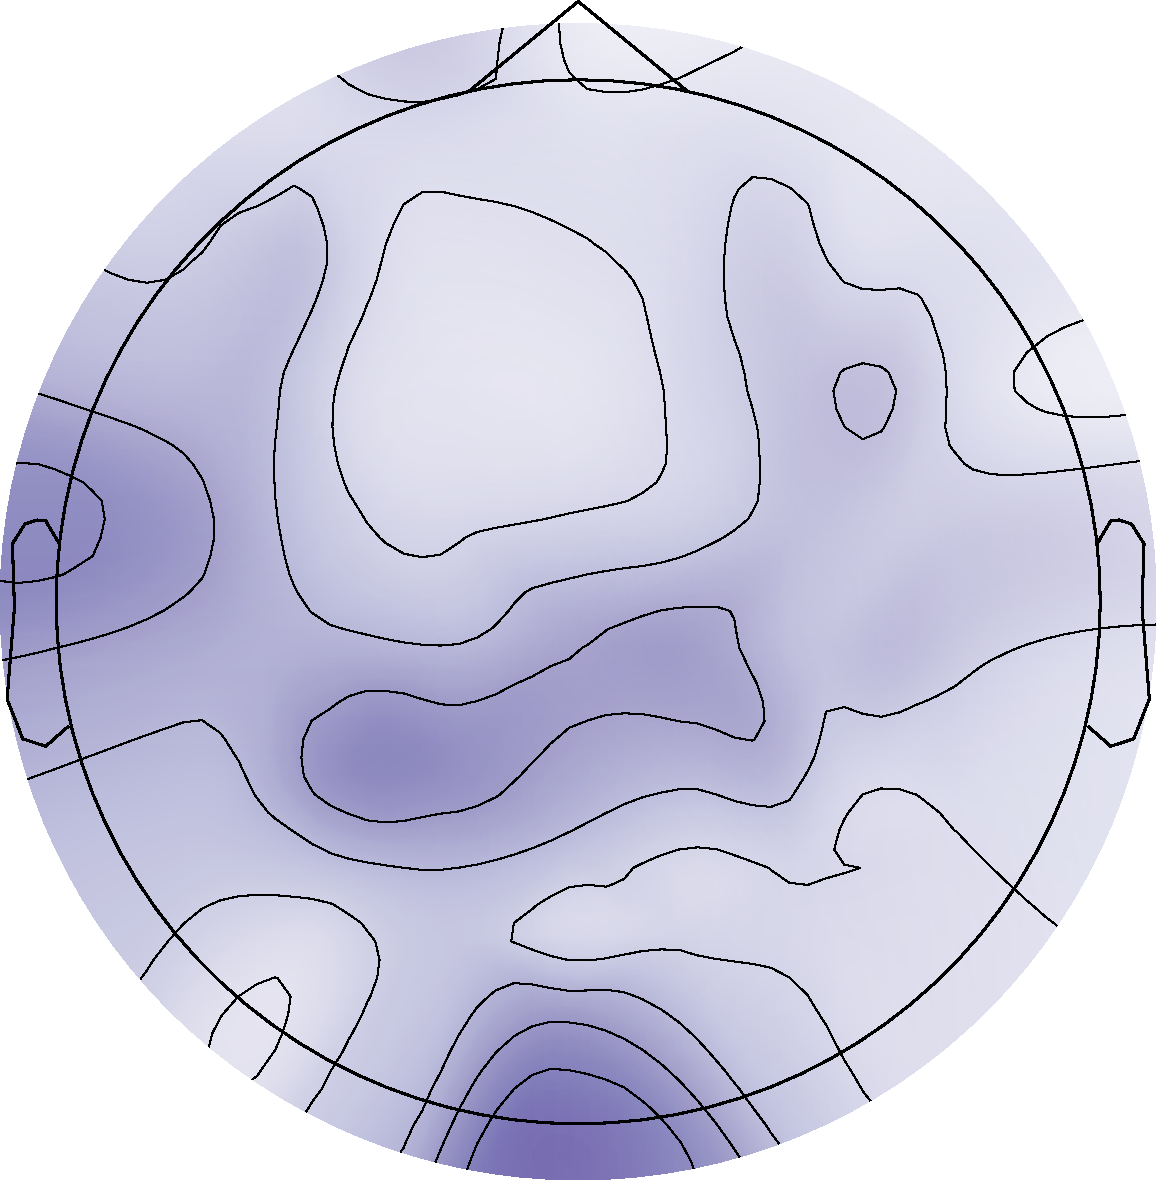
\includegraphics[width=\unitlength,page=1]{../Tesis_document/Figures/Objective_2/topoplot_weights_model_bad_2.pdf}}%
    \put(0.35967017,0.97370064){\color[rgb]{0,0,0}\makebox(0,0)[lt]{\lineheight{1.25}\smash{\begin{tabular}[t]{l} \Large Fp1\end{tabular}}}}%
    \put(0.48360239,0.98294885){\color[rgb]{0,0,0}\makebox(0,0)[lt]{\lineheight{1.25}\smash{\begin{tabular}[t]{l} \Large Fpz\end{tabular}}}}%
    \put(0.60675178,0.9772081){\color[rgb]{0,0,0}\makebox(0,0)[lt]{\lineheight{1.25}\smash{\begin{tabular}[t]{l} \Large Fp2\end{tabular}}}}%
    \put(0.25167316,0.91234234){\color[rgb]{0,0,0}\makebox(0,0)[lt]{\lineheight{1.25}\smash{\begin{tabular}[t]{l} \Large AF7\end{tabular}}}}%
    \put(0.35594816,0.90619712){\color[rgb]{0,0,0}\makebox(0,0)[lt]{\lineheight{1.25}\smash{\begin{tabular}[t]{l} \Large AF3\end{tabular}}}}%
    \put(0.4842652,0.90789149){\color[rgb]{0,0,0}\makebox(0,0)[lt]{\lineheight{1.25}\smash{\begin{tabular}[t]{l} \Large AFz\end{tabular}}}}%
    \put(0.6163543,0.90817342){\color[rgb]{0,0,0}\makebox(0,0)[lt]{\lineheight{1.25}\smash{\begin{tabular}[t]{l} \Large AF4\end{tabular}}}}%
    \put(0.71557323,0.91542903){\color[rgb]{0,0,0}\makebox(0,0)[lt]{\lineheight{1.25}\smash{\begin{tabular}[t]{l} \Large AF8\end{tabular}}}}%
    \put(0.19542921,0.7985205){\color[rgb]{0,0,0}\makebox(0,0)[lt]{\lineheight{1.25}\smash{\begin{tabular}[t]{l} \Large F7\end{tabular}}}}%
    \put(0.24637785,0.79532974){\color[rgb]{0,0,0}\makebox(0,0)[lt]{\lineheight{1.25}\smash{\begin{tabular}[t]{l} \Large F5\end{tabular}}}}%
    \put(0.31178444,0.79866219){\color[rgb]{0,0,0}\makebox(0,0)[lt]{\lineheight{1.25}\smash{\begin{tabular}[t]{l} \Large F3\end{tabular}}}}%
    \put(0.39486144,0.80350233){\color[rgb]{0,0,0}\makebox(0,0)[lt]{\lineheight{1.25}\smash{\begin{tabular}[t]{l} \Large F1\end{tabular}}}}%
    \put(0.48898264,0.80600112){\color[rgb]{0,0,0}\makebox(0,0)[lt]{\lineheight{1.25}\smash{\begin{tabular}[t]{l} \Large Fz\end{tabular}}}}%
    \put(0.58636438,0.8053206){\color[rgb]{0,0,0}\makebox(0,0)[lt]{\lineheight{1.25}\smash{\begin{tabular}[t]{l} \Large F2\end{tabular}}}}%
    \put(0.66805349,0.80209888){\color[rgb]{0,0,0}\makebox(0,0)[lt]{\lineheight{1.25}\smash{\begin{tabular}[t]{l} \Large F4\end{tabular}}}}%
    \put(0.74031021,0.80128649){\color[rgb]{0,0,0}\makebox(0,0)[lt]{\lineheight{1.25}\smash{\begin{tabular}[t]{l} \Large F6\end{tabular}}}}%
    \put(0.78864303,0.80554177){\color[rgb]{0,0,0}\makebox(0,0)[lt]{\lineheight{1.25}\smash{\begin{tabular}[t]{l} \Large F8\end{tabular}}}}%
    \put(0.15454614,0.67815348){\color[rgb]{0,0,0}\makebox(0,0)[lt]{\lineheight{1.25}\smash{\begin{tabular}[t]{l} \Large FT7\end{tabular}}}}%
    \put(0.20615046,0.67997528){\color[rgb]{0,0,0}\makebox(0,0)[lt]{\lineheight{1.25}\smash{\begin{tabular}[t]{l} \Large FC5\end{tabular}}}}%
    \put(0.28304215,0.68580018){\color[rgb]{0,0,0}\makebox(0,0)[lt]{\lineheight{1.25}\smash{\begin{tabular}[t]{l} \Large FC3\end{tabular}}}}%
    \put(0.37439787,0.69273645){\color[rgb]{0,0,0}\makebox(0,0)[lt]{\lineheight{1.25}\smash{\begin{tabular}[t]{l} \Large FC1\end{tabular}}}}%
    \put(0.48466778,0.69558642){\color[rgb]{0,0,0}\makebox(0,0)[lt]{\lineheight{1.25}\smash{\begin{tabular}[t]{l} \Large FCz\end{tabular}}}}%
    \put(0.59323573,0.69300187){\color[rgb]{0,0,0}\makebox(0,0)[lt]{\lineheight{1.25}\smash{\begin{tabular}[t]{l} \Large FC2\end{tabular}}}}%
    \put(0.6886396,0.68755139){\color[rgb]{0,0,0}\makebox(0,0)[lt]{\lineheight{1.25}\smash{\begin{tabular}[t]{l} \Large FC4\end{tabular}}}}%
    \put(0.76580849,0.68247882){\color[rgb]{0,0,0}\makebox(0,0)[lt]{\lineheight{1.25}\smash{\begin{tabular}[t]{l} \Large FC6\end{tabular}}}}%
    \put(0.81263914,0.68078985){\color[rgb]{0,0,0}\makebox(0,0)[lt]{\lineheight{1.25}\smash{\begin{tabular}[t]{l} \Large FT8\end{tabular}}}}%
    \put(0.15304429,0.55517309){\color[rgb]{0,0,0}\makebox(0,0)[lt]{\lineheight{1.25}\smash{\begin{tabular}[t]{l} \Large T7\end{tabular}}}}%
    \put(0.20793189,0.56319421){\color[rgb]{0,0,0}\makebox(0,0)[lt]{\lineheight{1.25}\smash{\begin{tabular}[t]{l} \Large C5\end{tabular}}}}%
    \put(0.27584929,0.57156861){\color[rgb]{0,0,0}\makebox(0,0)[lt]{\lineheight{1.25}\smash{\begin{tabular}[t]{l} \Large C3\end{tabular}}}}%
    \put(0.3745513,0.57777057){\color[rgb]{0,0,0}\makebox(0,0)[lt]{\lineheight{1.25}\smash{\begin{tabular}[t]{l} \Large C1\end{tabular}}}}%
    \put(0.48810392,0.58059817){\color[rgb]{0,0,0}\makebox(0,0)[lt]{\lineheight{1.25}\smash{\begin{tabular}[t]{l} \Large Cz\end{tabular}}}}%
    \put(0.60220502,0.57775964){\color[rgb]{0,0,0}\makebox(0,0)[lt]{\lineheight{1.25}\smash{\begin{tabular}[t]{l} \Large C2\end{tabular}}}}%
    \put(0.70116468,0.57214845){\color[rgb]{0,0,0}\makebox(0,0)[lt]{\lineheight{1.25}\smash{\begin{tabular}[t]{l} \Large C4\end{tabular}}}}%
    \put(0.77357975,0.56454438){\color[rgb]{0,0,0}\makebox(0,0)[lt]{\lineheight{1.25}\smash{\begin{tabular}[t]{l} \Large C6\end{tabular}}}}%
    \put(0.81934835,0.55648819){\color[rgb]{0,0,0}\makebox(0,0)[lt]{\lineheight{1.25}\smash{\begin{tabular}[t]{l} \Large T8\end{tabular}}}}%
    \put(0.15179749,0.43852829){\color[rgb]{0,0,0}\makebox(0,0)[lt]{\lineheight{1.25}\smash{\begin{tabular}[t]{l} \Large TP7\end{tabular}}}}%
    \put(0.20911869,0.45089969){\color[rgb]{0,0,0}\makebox(0,0)[lt]{\lineheight{1.25}\smash{\begin{tabular}[t]{l} \Large CP5\end{tabular}}}}%
    \put(0.27925225,0.45863264){\color[rgb]{0,0,0}\makebox(0,0)[lt]{\lineheight{1.25}\smash{\begin{tabular}[t]{l} \Large CP3\end{tabular}}}}%
    \put(0.37303221,0.46333493){\color[rgb]{0,0,0}\makebox(0,0)[lt]{\lineheight{1.25}\smash{\begin{tabular}[t]{l} \Large CP1\end{tabular}}}}%
    \put(0.48386986,0.4646749){\color[rgb]{0,0,0}\makebox(0,0)[lt]{\lineheight{1.25}\smash{\begin{tabular}[t]{l} \Large CPz\end{tabular}}}}%
    \put(0.59956022,0.4631065){\color[rgb]{0,0,0}\makebox(0,0)[lt]{\lineheight{1.25}\smash{\begin{tabular}[t]{l} \Large CP2\end{tabular}}}}%
    \put(0.69365939,0.45836548){\color[rgb]{0,0,0}\makebox(0,0)[lt]{\lineheight{1.25}\smash{\begin{tabular}[t]{l} \Large CP4\end{tabular}}}}%
    \put(0.76588935,0.45053079){\color[rgb]{0,0,0}\makebox(0,0)[lt]{\lineheight{1.25}\smash{\begin{tabular}[t]{l} \Large CP6\end{tabular}}}}%
    \put(0.81109972,0.43829568){\color[rgb]{0,0,0}\makebox(0,0)[lt]{\lineheight{1.25}\smash{\begin{tabular}[t]{l} \Large TP8\end{tabular}}}}%
    \put(0.14280779,0.28880769){\color[rgb]{0,0,0}\makebox(0,0)[lt]{\lineheight{1.25}\smash{\begin{tabular}[t]{l} \Large P9\end{tabular}}}}%
    \put(0.21177283,0.33788382){\color[rgb]{0,0,0}\makebox(0,0)[lt]{\lineheight{1.25}\smash{\begin{tabular}[t]{l} \Large P7\end{tabular}}}}%
    \put(0.25524798,0.34872785){\color[rgb]{0,0,0}\makebox(0,0)[lt]{\lineheight{1.25}\smash{\begin{tabular}[t]{l} \Large P5\end{tabular}}}}%
    \put(0.31471011,0.35396133){\color[rgb]{0,0,0}\makebox(0,0)[lt]{\lineheight{1.25}\smash{\begin{tabular}[t]{l} \Large P3\end{tabular}}}}%
    \put(0.39657699,0.35639073){\color[rgb]{0,0,0}\makebox(0,0)[lt]{\lineheight{1.25}\smash{\begin{tabular}[t]{l} \Large P1\end{tabular}}}}%
    \put(0.48761831,0.35703037){\color[rgb]{0,0,0}\makebox(0,0)[lt]{\lineheight{1.25}\smash{\begin{tabular}[t]{l} \Large Pz\end{tabular}}}}%
    \put(0.58532274,0.35619013){\color[rgb]{0,0,0}\makebox(0,0)[lt]{\lineheight{1.25}\smash{\begin{tabular}[t]{l} \Large P2\end{tabular}}}}%
    \put(0.66479928,0.35384699){\color[rgb]{0,0,0}\makebox(0,0)[lt]{\lineheight{1.25}\smash{\begin{tabular}[t]{l} \Large P4\end{tabular}}}}%
    \put(0.71635351,0.34901564){\color[rgb]{0,0,0}\makebox(0,0)[lt]{\lineheight{1.25}\smash{\begin{tabular}[t]{l} \Large P6\end{tabular}}}}%
    \put(0.75830552,0.33820045){\color[rgb]{0,0,0}\makebox(0,0)[lt]{\lineheight{1.25}\smash{\begin{tabular}[t]{l} \Large P8\end{tabular}}}}%
    \put(0.82302529,0.28323049){\color[rgb]{0,0,0}\makebox(0,0)[lt]{\lineheight{1.25}\smash{\begin{tabular}[t]{l} \Large P10\end{tabular}}}}%
    \put(0.27724394,0.25345665){\color[rgb]{0,0,0}\makebox(0,0)[lt]{\lineheight{1.25}\smash{\begin{tabular}[t]{l} \Large PO7\end{tabular}}}}%
    \put(0.35847051,0.27198285){\color[rgb]{0,0,0}\makebox(0,0)[lt]{\lineheight{1.25}\smash{\begin{tabular}[t]{l} \Large PO3\end{tabular}}}}%
    \put(0.48179514,0.27697386){\color[rgb]{0,0,0}\makebox(0,0)[lt]{\lineheight{1.25}\smash{\begin{tabular}[t]{l} \Large POz\end{tabular}}}}%
    \put(0.60260432,0.2713257){\color[rgb]{0,0,0}\makebox(0,0)[lt]{\lineheight{1.25}\smash{\begin{tabular}[t]{l} \Large PO4\end{tabular}}}}%
    \put(0.68406091,0.25242003){\color[rgb]{0,0,0}\makebox(0,0)[lt]{\lineheight{1.25}\smash{\begin{tabular}[t]{l} \Large PO8\end{tabular}}}}%
    \put(0.37725427,0.20621882){\color[rgb]{0,0,0}\makebox(0,0)[lt]{\lineheight{1.25}\smash{\begin{tabular}[t]{l} \Large O1\end{tabular}}}}%
    \put(0.48447457,0.20522474){\color[rgb]{0,0,0}\makebox(0,0)[lt]{\lineheight{1.25}\smash{\begin{tabular}[t]{l} \Large Oz\end{tabular}}}}%
    \put(0.59051709,0.20723652){\color[rgb]{0,0,0}\makebox(0,0)[lt]{\lineheight{1.25}\smash{\begin{tabular}[t]{l} \Large O2\end{tabular}}}}%
    \put(0.48585895,0.13245888){\color[rgb]{0,0,0}\makebox(0,0)[lt]{\lineheight{1.25}\smash{\begin{tabular}[t]{l} \Large Iz\end{tabular}}}}%
  \end{picture}%
\endgroup%
}
    \end{subfigure}
    \\
    \begin{subfigure}[b]{\linewidth}
        \centering
        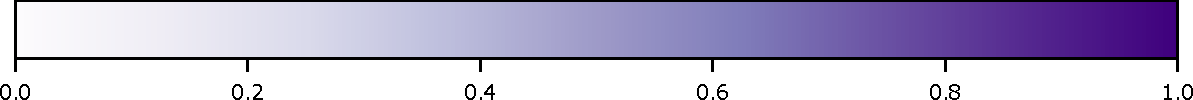
\includegraphics[width=\linewidth]{Figures/Objective_2/colorbar.pdf}
    \end{subfigure}
    \caption{KSC-FCnet functional connectivity results (Circos plots and topoplots). The first row illustrates the 99th percentile of the most significant functional connections across the centroid subjects concerning the studied best, medium, and worst performance clusters (see Figure \ref{fig:dataset_sensors}), with the opacity representing the strength of the connectivity. The second and third rows display topoplots of the two-sampled Kolmogorov--Smirnov test and the weights of the classification layer on the KCS-FCnet, respectively. The purer the purple color, the more important the brain area is. The left to right column represents each group from G I to G III.}
    \label{fig:topoplot_graphs}
\end{figure}

Table \ref{table:compmod} summarizes the results of KCS-FCnet and the contrasted end-to-end architectures of Convolutional neural network models. Deepconvnet performs the poorest, making it unsuitable for handling high intra-class variability. By contrast, Shallowconvnet and TCNet-Fusion have values of quality measures that are very close to each other, being more competitive. Despite this, KCS-FCnet achieves the highest scores, outperforming the other models.


Another essential aspect to quantify the model performance is the number of trainable parameters. Figure \ref{fig:paramsvsacc} presents the required number of trainable parameters vs. the attained MI classification performance for each studied DL approach. As seen, a higher number of trainable parameters does not necessarily imply a higher classification accuracy. In fact, two clusters are evident: models holding less than 20k trainable parameters and algorithms requiring more than 100k parameters. Notably, the EEGnet gathers 2.194 trainable parameters and got a $69\%$ accuracy score. Then,  the Deepconvnet has the most significant number of trainable parameters (178.927) but only achieves a $62.5\%$ accuracy score. The overfitting issue can explain the latter, especially when dealing with a high intra-class variability MI dataset. As previously stated, the Shallowconvnet, TCNet-Fusion, and KCS-FCnet have the highest accuracy scores. However, the Shallowconvnet has more than 100k trainable parameters, and the TCNet-Fusion has more than 25k. Conversely, our KCS-FCnet, not only outperforms these architectures in terms of accuracy but also requires the lowest complexity to achieve competitive discrimination results.

\begin{table}[H]
    \caption{Method Comparison results regarding the average MI classification for the Giga database.}\label{table:compmod}
    \centering
    \begin{tabular}{lccc}
        \toprule
        \textbf{Approach}         &  \textbf{Accuracy}  & \textbf{Kappa}  & \textbf{AUC}  \\ 
        \midrule
        Deepconvnet~\cite{schirrmeister2017deep}    & $62.5 \pm 13.0$  & $24.5 \pm 25.9$   & $68.9 \pm 17.8$  \\ 
        EEGnet~\cite{lawhern2018eegnet}             & $69.0 \pm 14.6$  & $38.0 \pm 29.1$   & $75.4 \pm 16.6$  \\ 
        TCNet-Fusion~\cite{musallam2021electroencephalography}   & $72.7 \pm 14.0$  & $45.0 \pm 28.2$   & $79.6 \pm 15.9$  \\ 
        Shallowconvnet~\cite{schirrmeister2017deep} & $74.9 \pm 13.9$  & $49.5 \pm 27.8$   & $79.9 \pm 15.1$  \\ 
        \midrule
        KCS-FCnet                   & \textbf{$76.4 \pm 11.3$}  &  \textbf{$52.6 \pm 22.7$}  & \textbf{$82.2 \pm 12.2$}  \\ 
        \bottomrule
    \end{tabular}
\end{table}

\vspace{-6pt}
%%acc vs. #parameters
\begin{figure}[h!]
    \centering
    \resizebox{0.9\linewidth}{!}{% This file was created with tikzplotlib v0.10.1.
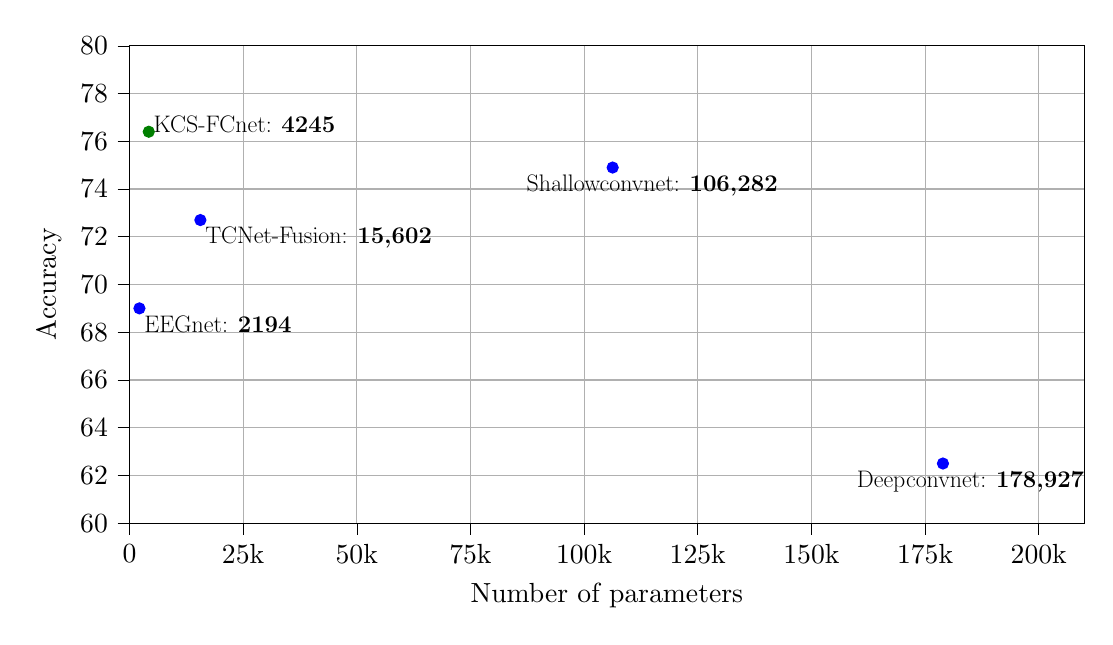
\begin{tikzpicture}

\definecolor{darkgray176}{RGB}{176,176,176}
\definecolor{green01270}{RGB}{0,127,0}

\begin{axis}[
tick align=outside,
tick pos=left,
x grid style={darkgray176},
xlabel={Number of parameters},
ylabel={Accuracy},
xmin=0, xmax=210000,
xtick style={color=black},
xtick={0,25000,50000,75000,100000,125000,150000,175000,200000},
xticklabels={0,25k,50k,75k,100k,125k,150k,175k,200k},
y grid style={darkgray176},
ymin=60, ymax=80,
ytick = {60,62,64,66,68,70,72,74,76,78,80},
ytick style={color=black},
grid=both,
%ymajorgrids=true,
% only scale the axis, not the axis including the ticks and labels
scale only axis=true,
scaled x ticks = false,
% set `width' and `height' to the desired values
width=\textwidth,
height=0.5\textwidth,
]
%\draw[step=5mm,black!15!white, very thin] (0,60) grid (200000,80);
\addplot [draw=blue, draw=none, fill=blue, mark=*]
table{%
x  y
2194 69
};
\addplot [draw=green01270, draw=none, fill=green01270, mark=*]
table{%
x  y
4245 76.4
};
\addplot [draw=blue, draw=none, fill=blue, mark=*]
table{%
x  y
178927 62.5
};
\addplot [draw=blue, draw=none, fill=blue, mark=*]
table{%
x  y
106282 74.9
};
\addplot [draw=blue, draw=none, fill=blue, mark=*]
table{%
x  y
15602 72.7
};
\draw (axis cs:2194,68) node[
  scale=0.5,
  anchor=base west,
  text=black,
  rotate=0.0
]{\LARGE{EEGnet:  \textbf{2194}}};
\draw (axis cs:4245,76.37) node[
  scale=0.5,
  anchor=base west,
  text=black,
  rotate=0.0
]{\LARGE{KCS-FCnet:  \textbf{4245}}};
\draw (axis cs:158927,61.5) node[
  scale=0.5,
  anchor=base west,
  text=black,
  rotate=0.0
]{\LARGE{Deepconvnet:  \textbf{178,927}}};
\draw (axis cs:86282,73.9) node[
  scale=0.5,
  anchor=base west,
  text=black,
  rotate=0.0
]{\LARGE{Shallowconvnet:  \textbf{106,282}}};
\draw (axis cs:15602,71.7) node[
  scale=0.5,
  anchor=base west,
  text=black,
  rotate=0.0
]{\LARGE{TCNet-Fusion:  \textbf{15,602}}};
\end{axis}

\end{tikzpicture}
}
    \caption{{Method}
        comparison results: number of trainable parameters vs. average motor imagery classification accuracy for the Giga database.}\label{fig:paramsvsacc}
\end{figure}


\section{Summary}

We have designed a novel end-to-end DL EEG-based MI classification method, termed the Kernel Cross-Spectral Functional Connectivity Network (KCS-FCnet). This strategy directly addresses fundamental issues like the elimination of handcrafted feature extraction steps and artifact removal that often generate false connectivities, as elaborated in \cref{sec:problem2}. Our methodology combines cross-spectral analysis with a data-driven KCS-FC block to model the non-linear connections between different channels and a CNN layer to automatically refine temporal, spectral, and spatial representations from EEGs. We appraised the efficacy of our approach alongside other end-to-end DL techniques using an extensively utilized public dataset. The results demonstrated that our KCS-FCnet approach consistently outperforms prevalent state-of-the-art methods in terms of both EEG-based MI classification and spatio-temporal-frequency interpretability. This system also minimizes the number of trainable parameters, thus reducing architectural complexity.

Although our approach outperforms other DL solutions when it comes to accuracy, it remains a challenge to conclusively affirm if our system offers enhanced interpretability as discussed in \cref{sec:problem3}. To ensure a comprehensive analysis of the interpreted results, it is essential to employ both qualitative and quantitative methodologies. Future studies, as suggested in \cref{sec:sota3}, should aim to incorporate post-hoc and intrinsic strategies to develop MI-BCI models that are more transparent and interpretable.